\documentclass{article}
\usepackage{titling}
\usepackage{graphicx}
\usepackage{caption}
\usepackage{subcaption}
\graphicspath{{graphics/}{../traffic_data_analysis/traffic_data_analysis/plots/}}

\pretitle{
  \begin{center}
  \huge
  
\includegraphics[width=10cm]{graphics/PSU_logo_transparent.png}\\[\bigskipamount]
}
\posttitle{\end{center}}
\usepackage{amsfonts}
\usepackage{booktabs}
\usepackage{longtable}
\usepackage{array}
\usepackage{multirow}
\usepackage{wrapfig}
\usepackage{float}
\usepackage{colortbl}
\usepackage{pdflscape}
\usepackage{tabu}
\usepackage{threeparttable}
\usepackage{xcolor}
\usepackage{soul}
\usepackage{fancyhdr}
\usepackage{hyperref}
\usepackage{float}
\pagestyle{fancy}
\rhead{
\includegraphics[width = .05\textwidth]{graphics/psulogo2.jpg}}
\usepackage{geometry}
\geometry{a4paper, margin=0.75in}

\title{Portland Traffic Analysis: Final Report}
\author{
  Xu, Suru\\
  \texttt{suru@pdx.edu}
  \and
  Nelson, Austen\\
  \texttt{ajn6@pdx.edu}
}

\date{\today}

\begin{document}

\maketitle

\tableofcontents

\section{Executive Summary}

\section{Introduction}

\section{Background}

\section{Data}

The data we analyzed consists of vehicle counts over hourly time periods at 12 different highway locations, each consisting of 2 opposite directions (either NB/SB or EB/WB). Some locations have many more years available than others but in total there are about 3.2 million hours of data recorded over the 24 location and direction combinations. For a visual of the data coverage for each location / direction combination, see figure \ref{fig:data_availability}.

Many trends and area specific patterns can be easily identified by simply looking at the median values in the data. Table \ref{tab:medians} presents an approximation to weekday peak-time and peak-volume based on cubic periodic spline interpolation of hourly medians. 

General visible trends seem to be a slightly later peak traffic time in the mornings and location dependent changes in afternoon peak times. The peak volume is lower post-Covid all across the board, with very few exceptions outside of data availability issues. Lastly, looking at the occasional near-hour shift for some peak times (see Vista Ridge EB 2018, Wilsonville SB 2024, and Interstate Bridge NB 2024) indicates that there are potentially issues with Day Light Savings inconsistencies in the dataset. Duplicated hours (UTC time / no timezone) in the raw data additionally supports this hypothesis; so large changes in peak times may not be real in some cases.

\section{Methods}

\subsection{Generalized Additive Model (GAM)}

We have a dataset $D := \{x_i, y_i\}_{i=1}^n$, where $x_i$ is an hour in the day and $y_i$ is the observed number of cars in that hour. As expected, the correlation between the traffic volume and the time of the day is strong, with clear distinct patterns emerging for a different locations/directions and days of the week. To isolate different variables to make conclusions about changes in hourly traffic dynamics, we seek to create a simple model to summarize characteristics of interest. In particular, we are interested in how the rush hour has changed before and after the 2019 pandemic.

One of the most simple but powerful models in data science is linear regression, but as the name suggests isn't suitable for capturing non-linear relationships in data on its own. A common technique to address this constraint is to choose a suitable non-linear mapping such that the mapped inputs can be modeled with linear regression. GAMs are a class of Generalized Linear Models which provides a framework for selecting such a mapping as the sum over \emph{smooth} functions. The smoothness of these functions is desirable for our application because traffic volume as a function of time is ``smooth'' and we may be interested in rate characteristics of this function which can be obtained through differentiation (since smooth functions are differentiable). 

The GAM literature and software packaging calls these smooth function `smoothers' and many different functions are provided, but we are mostly interested in splines. Spline fitting is similar to fitting polynomials to the data but are generally easier to work with for a variety of reasons (see Runge effect, sklearn example). 

\subsection{Maximum Mean Discrepancy (MMD)}

\section{Results}

\subsection{Generalized Additive Model (GAM)}

\subsection{Maximum Mean Discrepancy (MMD)}

\section{Conclusions}

\appendix

\section{Median Peak Time and Volumes}

\definecolor{Gray}{gray}{0.9}
\newcolumntype{g}{>{\columncolor{Gray}}r}
\begin{figure}[H]
\captionof{table}{Weekday Peak Time Table} \label{tab:medians} 
\begin{tabular}{l l *{9}{g}}
    \toprule
    \rowcolor{white}
    \multicolumn{3}{c}{\textbf{Location Info}} & 
    \multicolumn{4}{c}{\textbf{Median Peak Time}} & 
    \multicolumn{4}{c}{\textbf{Median Peak Volume}}\\

    \cmidrule(lr){1-3} \cmidrule(lr){4-7} \cmidrule(lr){8-11}

    \rowcolor{white}
    \textbf{ID} & \textbf{Name} & \textbf{Dir} & 
    \textbf{2018} & \textbf{2019} & \textbf{2023} & \textbf{2024} &
    \textbf{2018} & \textbf{2019} & \textbf{2023} & \textbf{2024}\\ 

    \cmidrule(lr){1-3} \cmidrule(lr){4-7} \cmidrule(lr){8-11}

    \rowcolor{white}\rule{0pt}{4ex}
\multirow{2}{*}{34007} & \multirow{2}{*}{North Plains} &EB & 06:35 & 06:38 & 06:49 & 06:52 & 918 & 939 & 797 & 811 \\
& & WB & 16:06 & 16:03 & 15:49 & 15:55 & 1145 & 1166 & 1121 & 1167 \\
\rowcolor{white}\rule{0pt}{4ex}
\multirow{2}{*}{26022} & \multirow{2}{*}{Lents} &SB & 15:09 & 16:32 & 16:29 & 16:32 & 5521 & 5542 & 5250 & 5187 \\
& & NB & 06:23 & 06:26 & 07:01 & 06:58 & 5055 & 5060 & 5152 & 5111 \\
\rowcolor{white}\rule{0pt}{4ex}
\multirow{2}{*}{26002} & \multirow{2}{*}{Vista Ridge Tunne} &EB & 06:38 & 07:38 & 07:21 & 07:27 & 5047 & 4953 & 4695 & 4602 \\
& & WB & 07:15 & 07:18 & 15:34 & 07:24 & 5623 & 5612 & 5169 & 5173 \\
\rowcolor{white}\rule{0pt}{4ex}
\multirow{2}{*}{26001} & \multirow{2}{*}{Troutdale} &WB & 14:34 & 14:19 & 14:51 & 14:48 & 1229 & 1311 & 1266 & 1294 \\
& & EB & 10:26 & 10:40 & 10:11 & 10:08 & 1286 & 1368 & 1279 & 1331 \\
\rowcolor{white}\rule{0pt}{4ex}
\multirow{2}{*}{26004} & \multirow{2}{*}{Interstate Bridge} &SB & 06:29 & 05:34 & 06:09 & 06:06 & 1908 & 5609 & 5224 & 4939 \\
& & NB & 16:32 & 16:09 & 16:06 & 16:44 & 4619 & 4805 & 4625 & 4380 \\
\rowcolor{white}\rule{0pt}{4ex}
\multirow{2}{*}{26028} & \multirow{2}{*}{Fairview} &EB & 16:29 & 16:35 & 16:18 & 16:29 & 4493 & 4532 & 4391 & 4369 \\
& & WB & 06:29 & 06:35 & 06:41 & 06:35 & 4034 & 4064 & 3850 & 3761 \\
\rowcolor{white}\rule{0pt}{4ex}
\multirow{2}{*}{26024} & \multirow{2}{*}{Glenn Jackson Bridge} &NB & 15:06 & 15:06 & 15:06 & 14:45 & 7168 & 7137 & 6728 & 6614 \\
& & SB & 06:15 & 06:18 & 06:44 & 06:20 & 7411 & 7354 & 6188 & 6159 \\
\rowcolor{white}\rule{0pt}{4ex}
\multirow{2}{*}{34010} & \multirow{2}{*}{Beaverton-Bethany} &EB & 16:03 & 16:03 & 06:49 & 06:49 & 4521 & 4464 & 4191 & 4211 \\
& & WB & 07:15 & 07:15 & 16:21 & 16:24 & 4975 & 5152 & 4500 & 4531 \\
\rowcolor{white}\rule{0pt}{4ex}
\multirow{2}{*}{3011} & \multirow{2}{*}{Wilsonville} &SB & 14:57 & 14:57 & 14:37 & 15:40 & 3778 & 3791 & 3625 & 3640 \\
& & NB & 05:57 & 05:54 & 06:06 & 06:03 & 3832 & 3837 & 3756 & 3871 \\
\rowcolor{white}\rule{0pt}{4ex}
\multirow{2}{*}{26014} & \multirow{2}{*}{Hoyt} &WB & 05:40 & 05:37 & 06:03 & 06:03 & 5850 & 5809 & 5344 & 5363 \\
& & EB & 13:56 & 13:51 & 13:45 & 13:42 & 5587 & 5569 & 5283 & 5247 \\
\rowcolor{white}\rule{0pt}{4ex}
\multirow{2}{*}{3016} & \multirow{2}{*}{Stafford} &NB & 13:59 & 14:05 & 14:05 & 14:05 & 3267 & 3411 & 3186 & 3283 \\
& & SB & 06:23 & 06:23 & 06:55 & 06:55 & 3353 & 3367 & 3222 & 3309 \\
\rowcolor{white}\rule{0pt}{4ex}
\multirow{2}{*}{26016} & \multirow{2}{*}{Iowa Street} &SB & 16:32 & 16:29 & 16:29 & 16:26 & 5374 & 5339 & 4786 & 4758 \\
& & NB & 06:29 & 06:32 & 07:12 & 07:09 & 5687 & 5671 & 5303 & 5231 \\

\end{tabular}\par 
\bigskip 
    Hourly median traffic volume for each entry (location, direction, year) for weekdays is interpolated with a cubic spline to find approximate peak traffic time.
\end{figure}

\section{Data Availability}

\begin{figure}[H] 
    \centering
    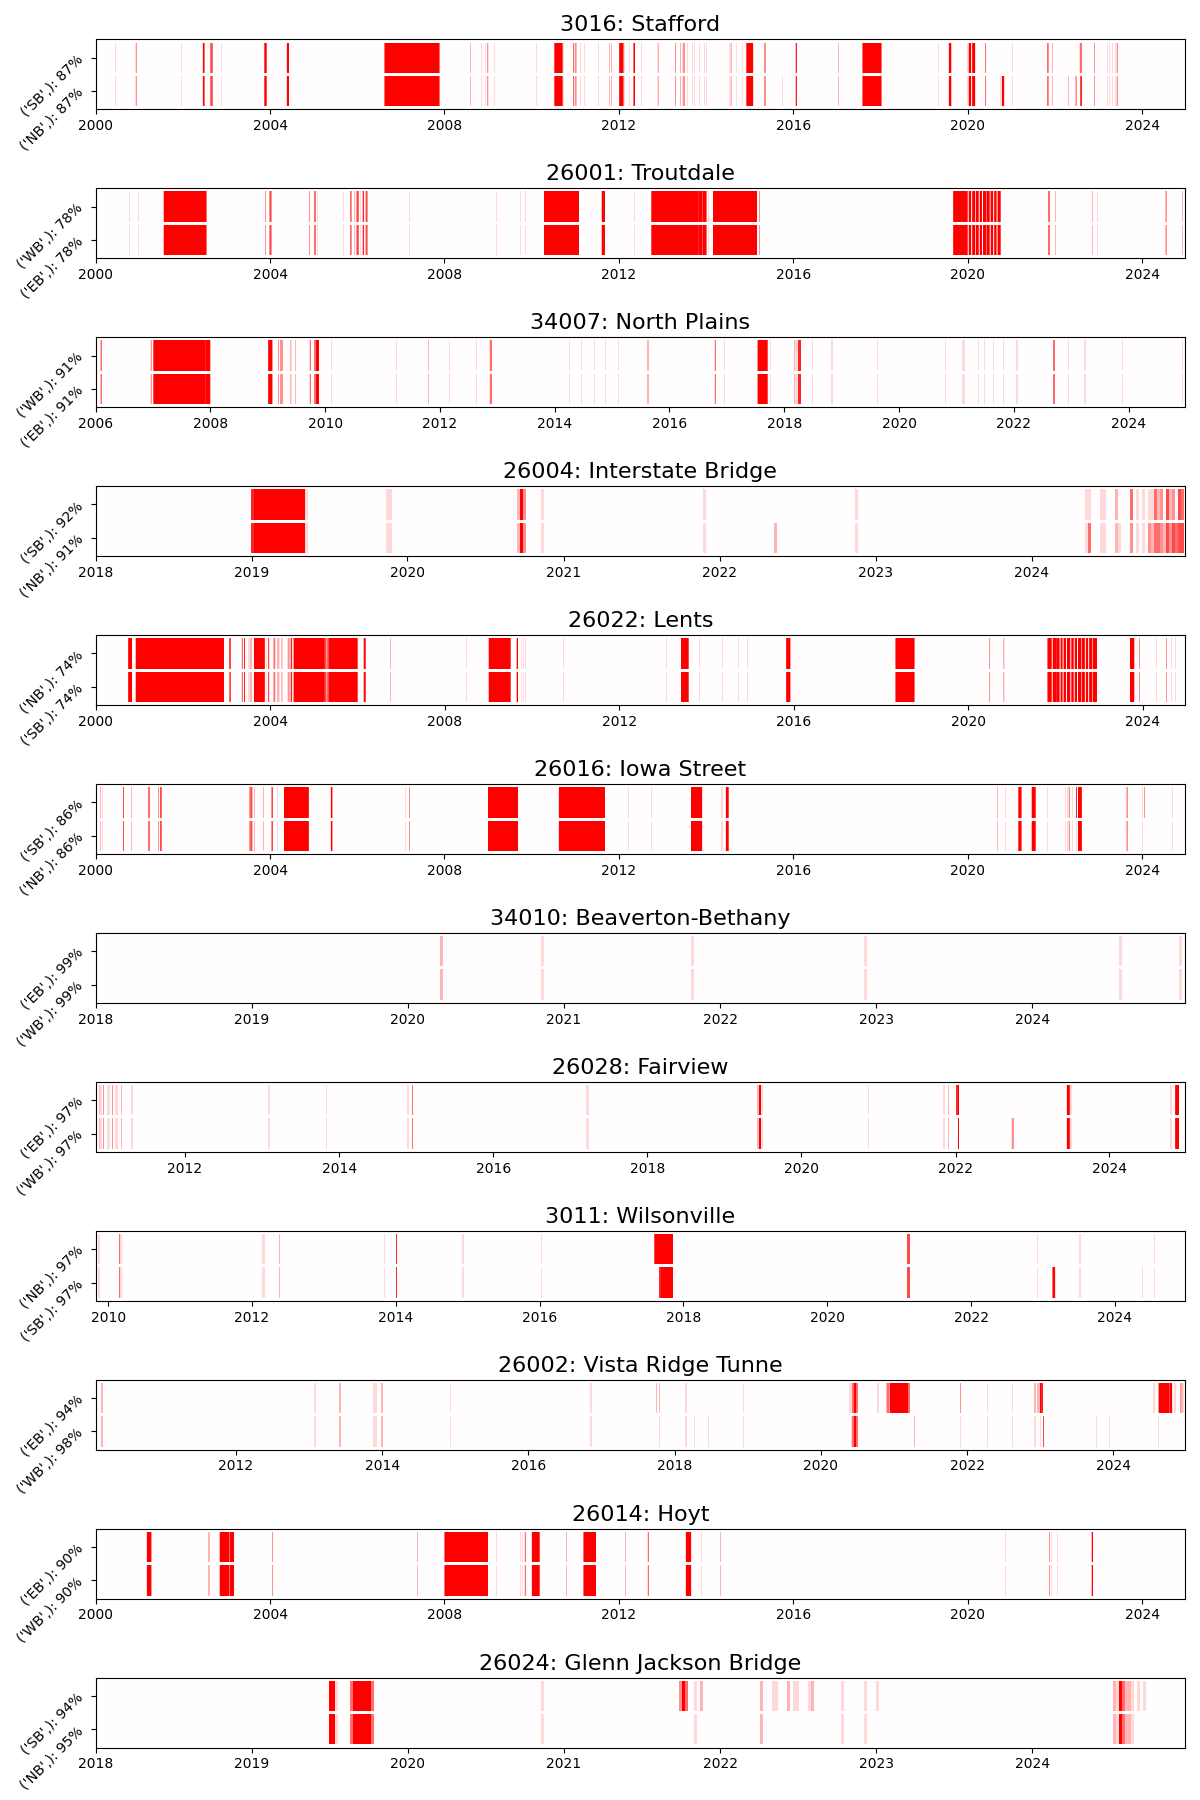
\includegraphics[width=0.9\textwidth]{missing_data.png}
    \caption{Red indicates missing data, opacity indicates how much of that week is missing. This doesn't account for ``0'' data which is technically missing and misrepresented.}
    \label{fig:data_availability}
\end{figure}

\section{Smooth Hourly Trends} 

These plots provide a visual for similar data presented in table \ref{tab:medians} but includes every year available in the dataset with quantile shading. Each line is the periodic cubic spline interpolation of the hourly medians/quantiles for each (location, direction, weekday/weekend) tuple. Some strange data issues become apparent in these plots, but they are almost entirely only in years we aren't concerned with in this analysis.
\begin{figure}[htbp]
	\centering
	\begin{subfigure}{0.45\textwidth}
		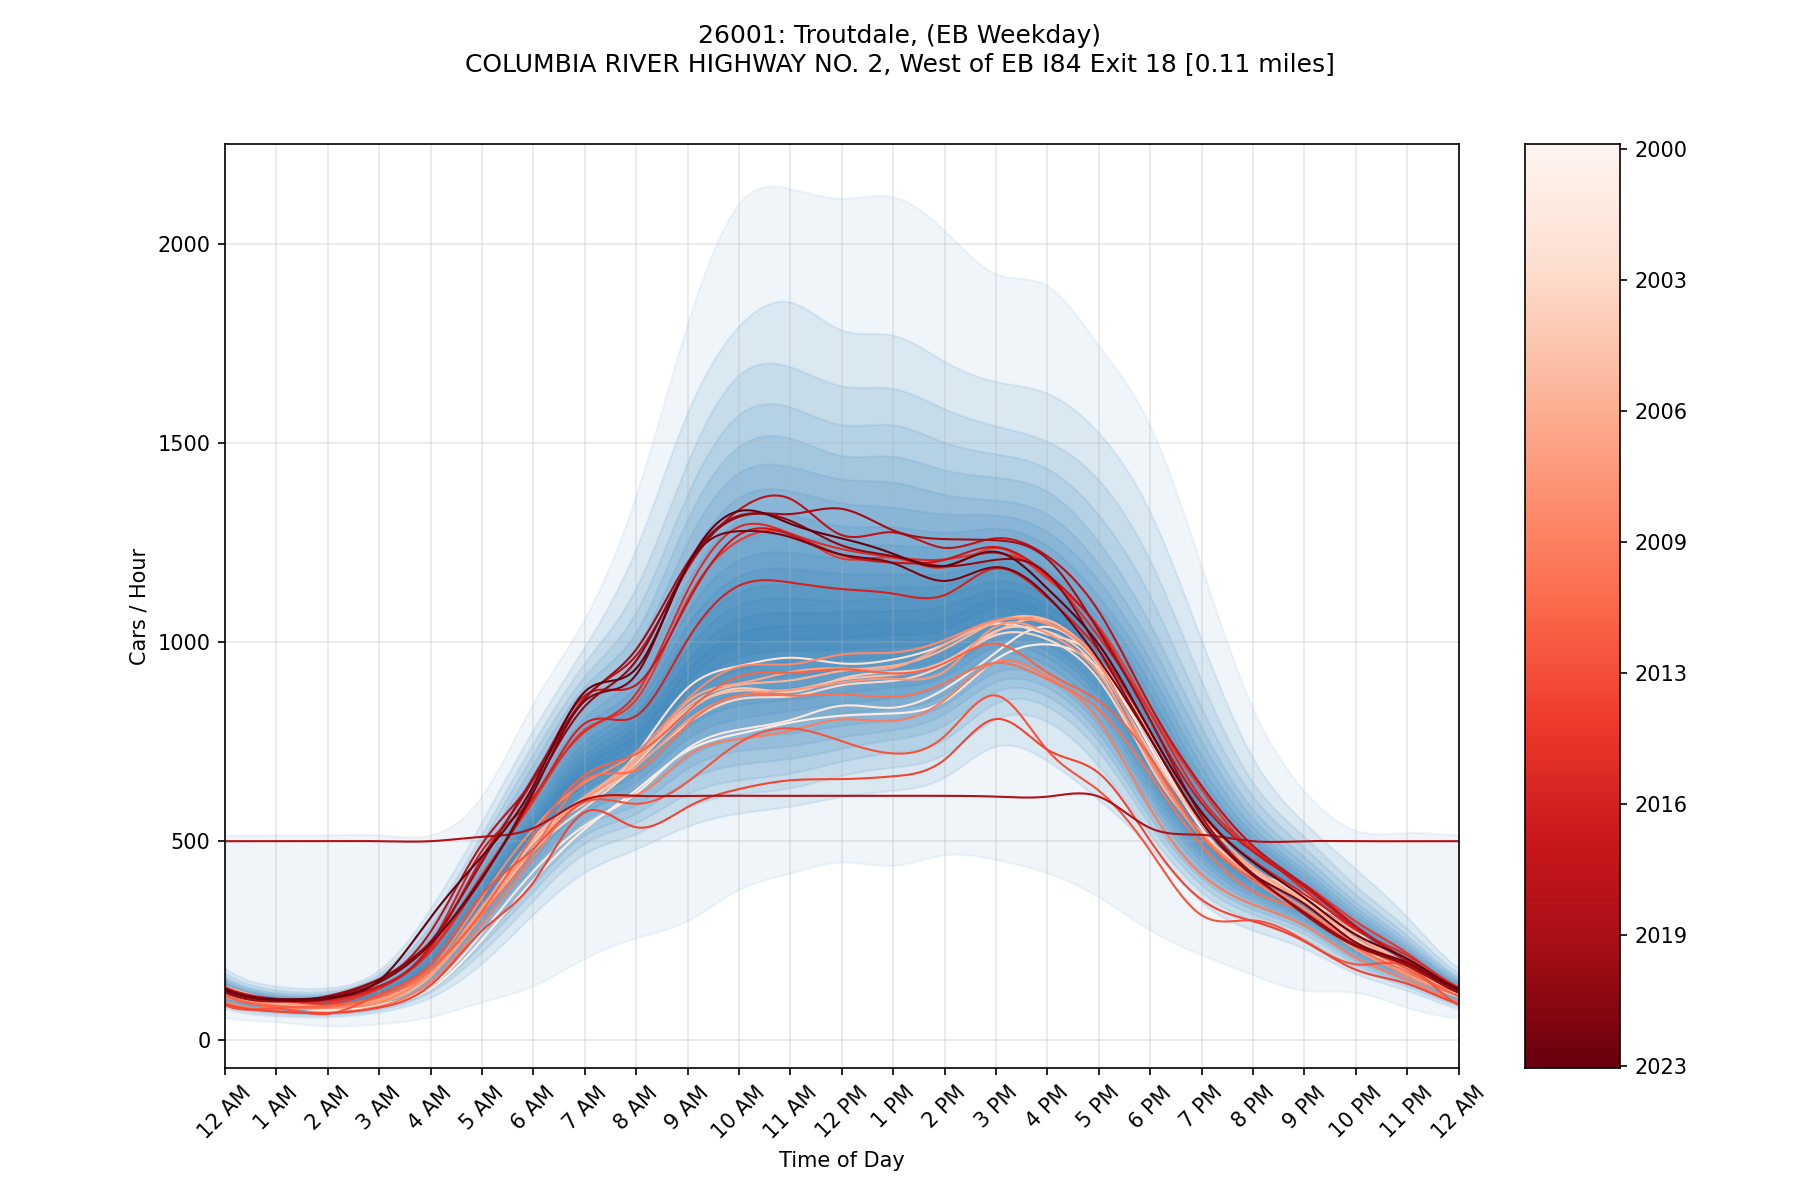
\includegraphics[width=\textwidth]{26001_Troutdale_EB_Weekday.png}
	\end{subfigure}
	\hfill
	\begin{subfigure}{0.45\textwidth}
		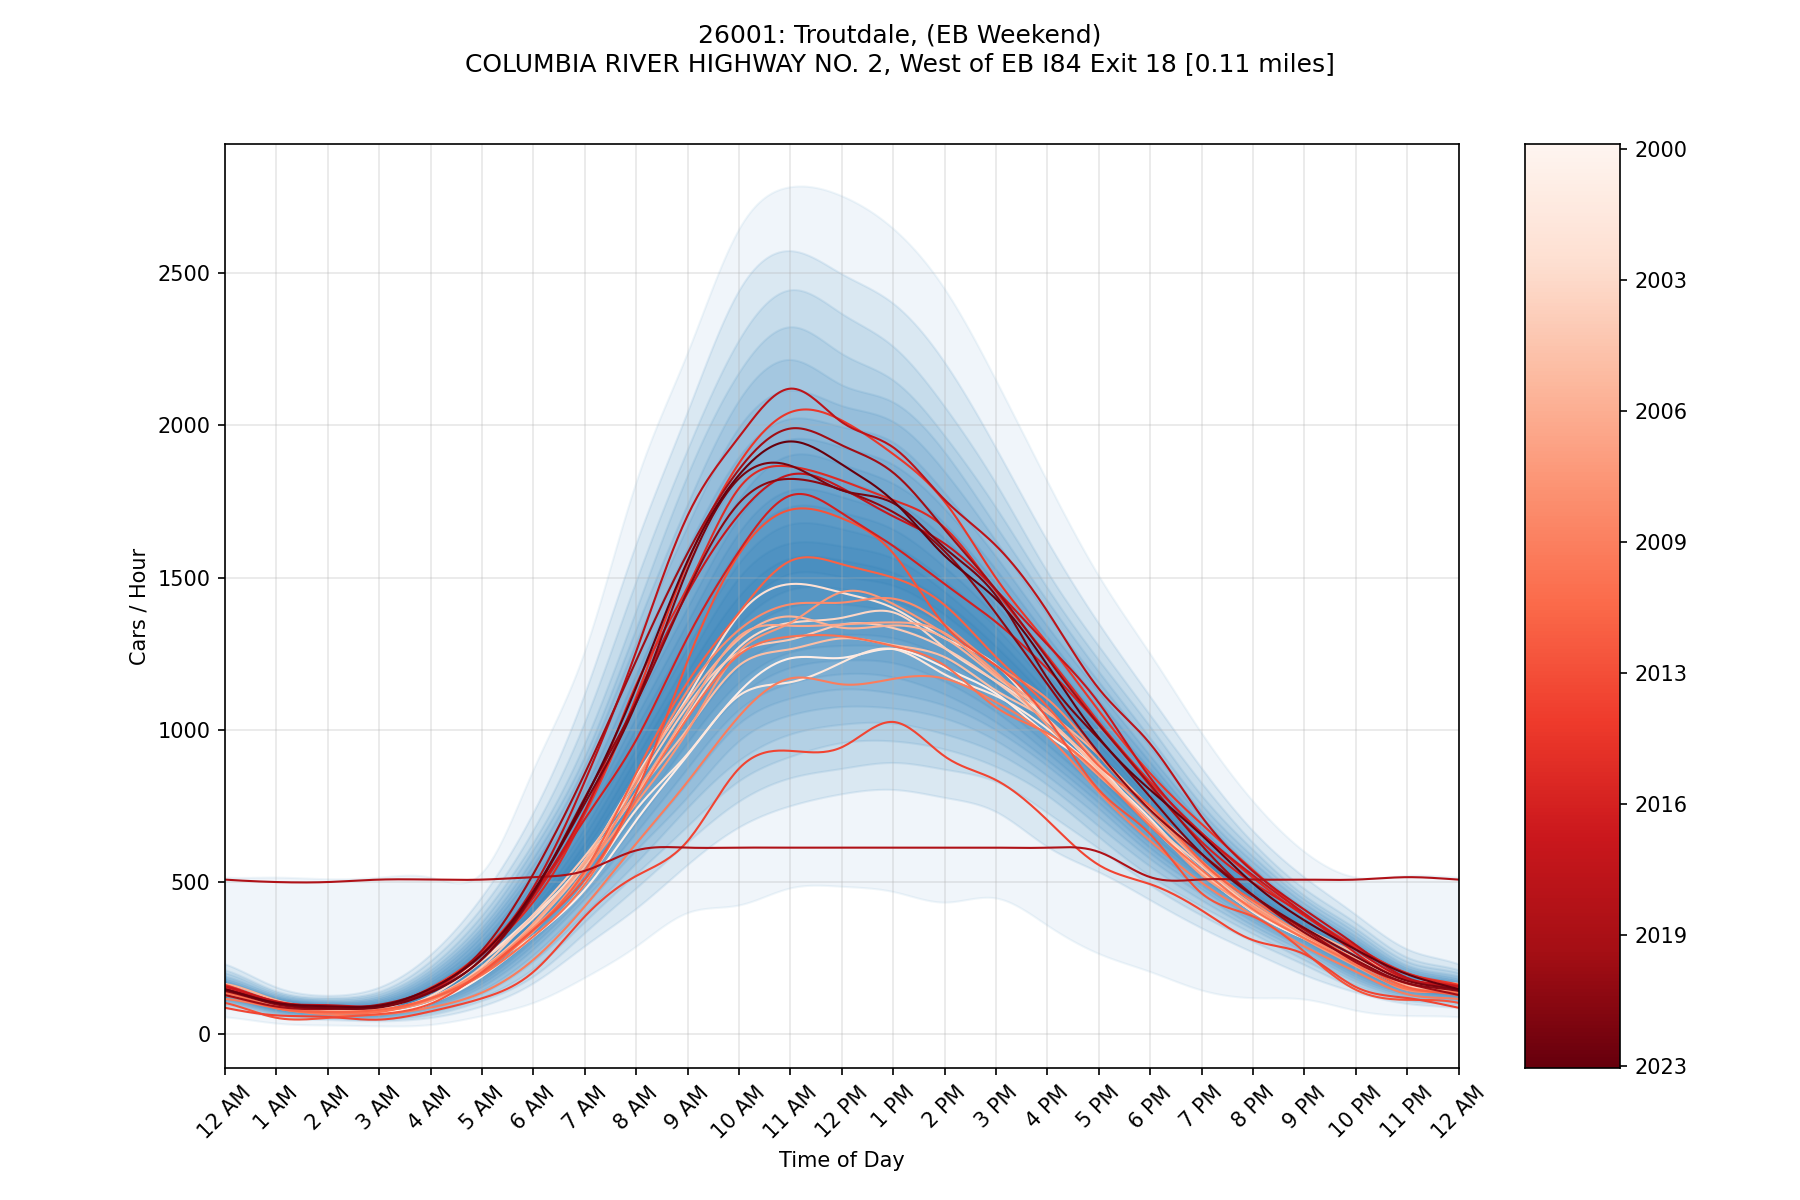
\includegraphics[width=\textwidth]{26001_Troutdale_EB_Weekend.png}
	\end{subfigure}

	\begin{subfigure}{0.45\textwidth}
		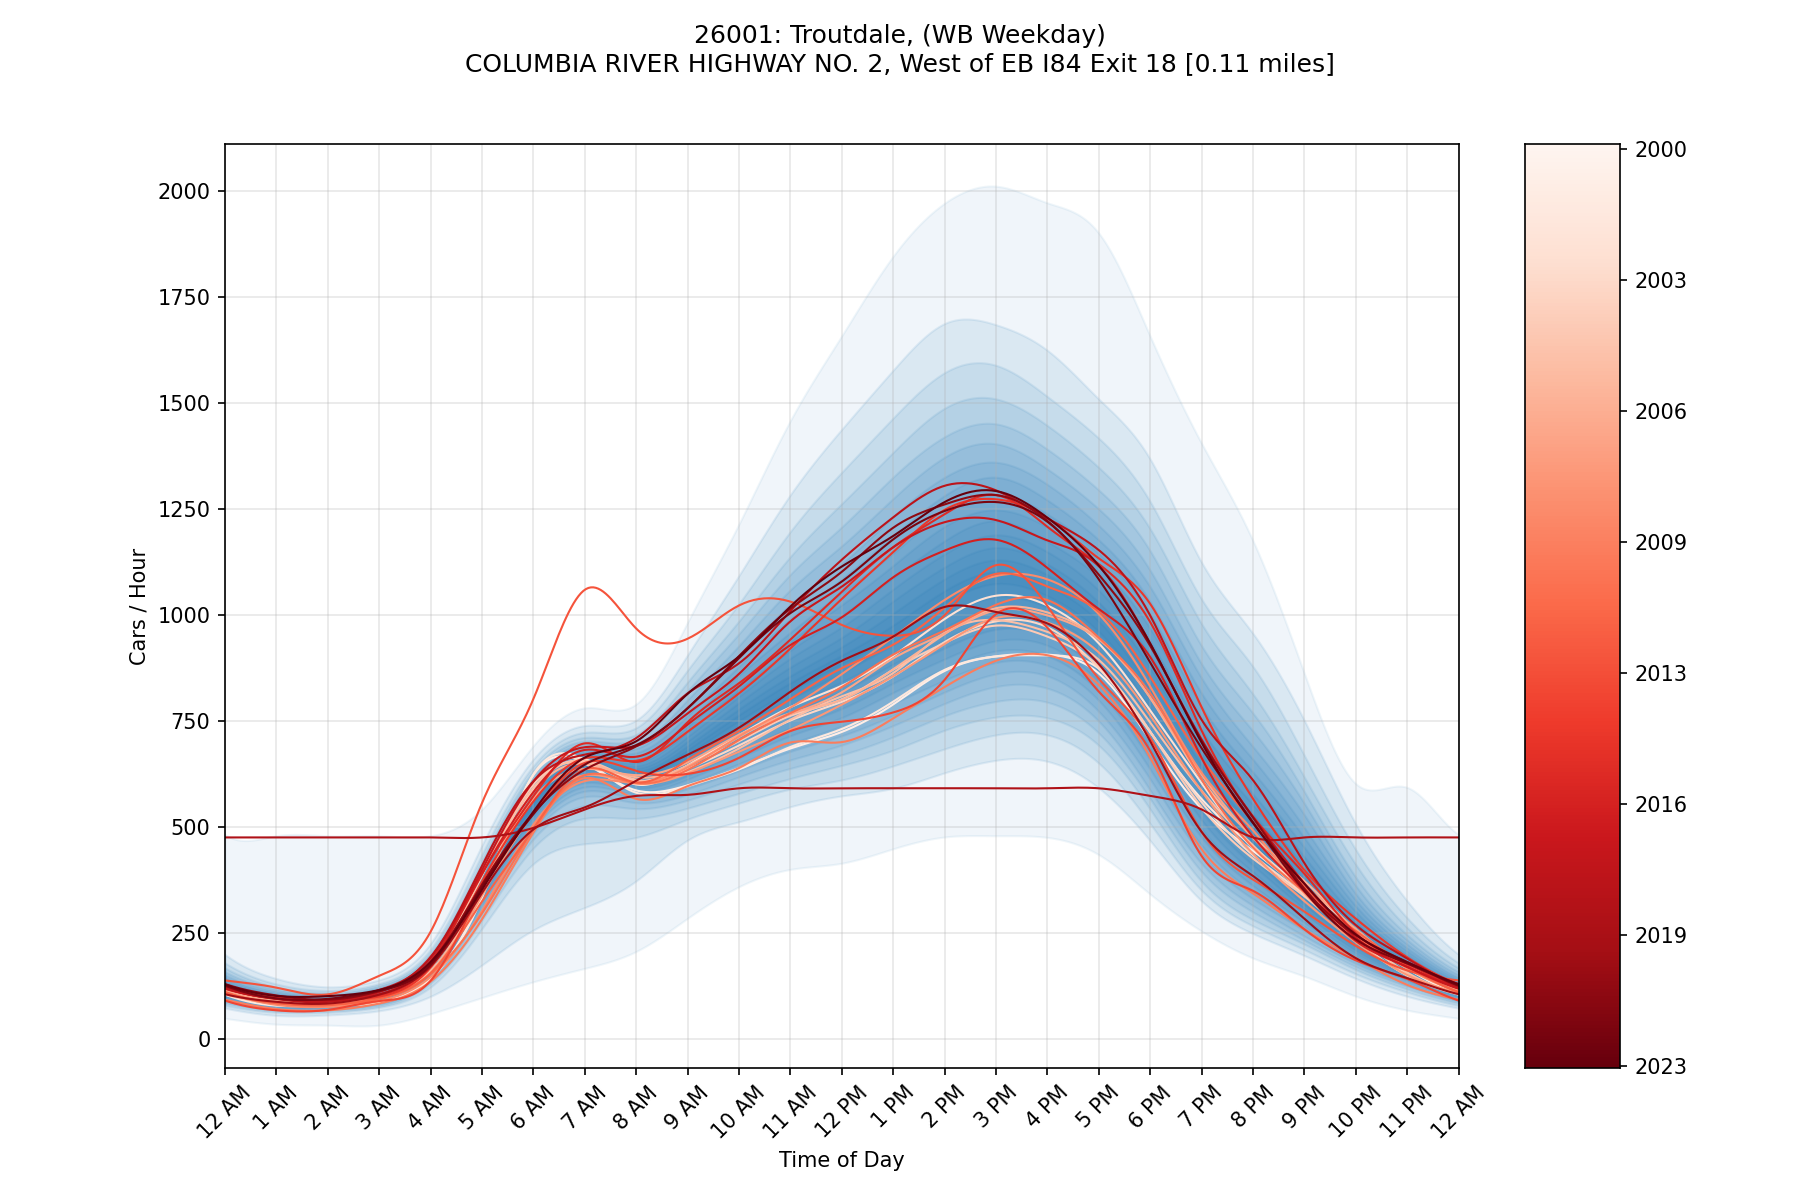
\includegraphics[width=\textwidth]{26001_Troutdale_WB_Weekday.png}
	\end{subfigure}
	\hfill
	\begin{subfigure}{0.45\textwidth}
		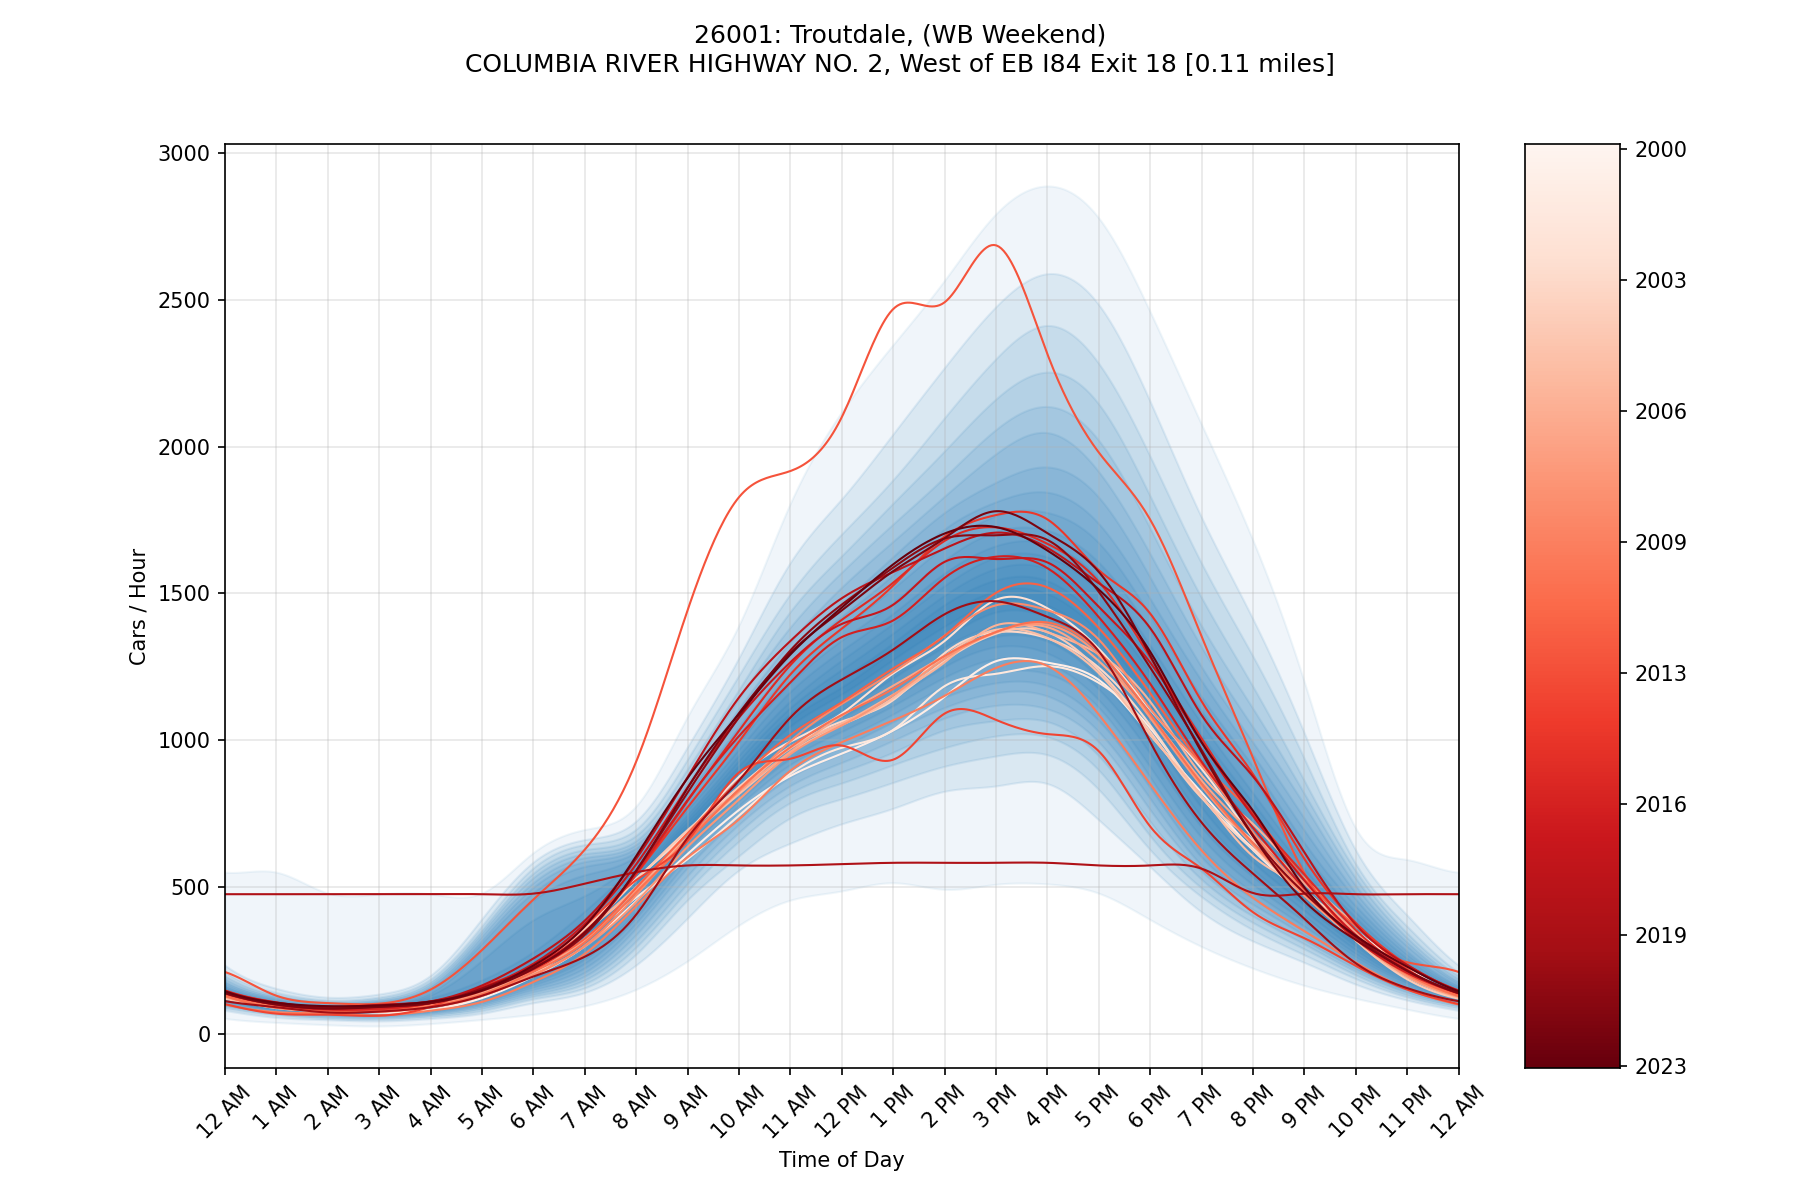
\includegraphics[width=\textwidth]{26001_Troutdale_WB_Weekend.png}
	\end{subfigure}
\end{figure}

\begin{figure}[htbp]
	\centering
	\begin{subfigure}{0.45\textwidth}
		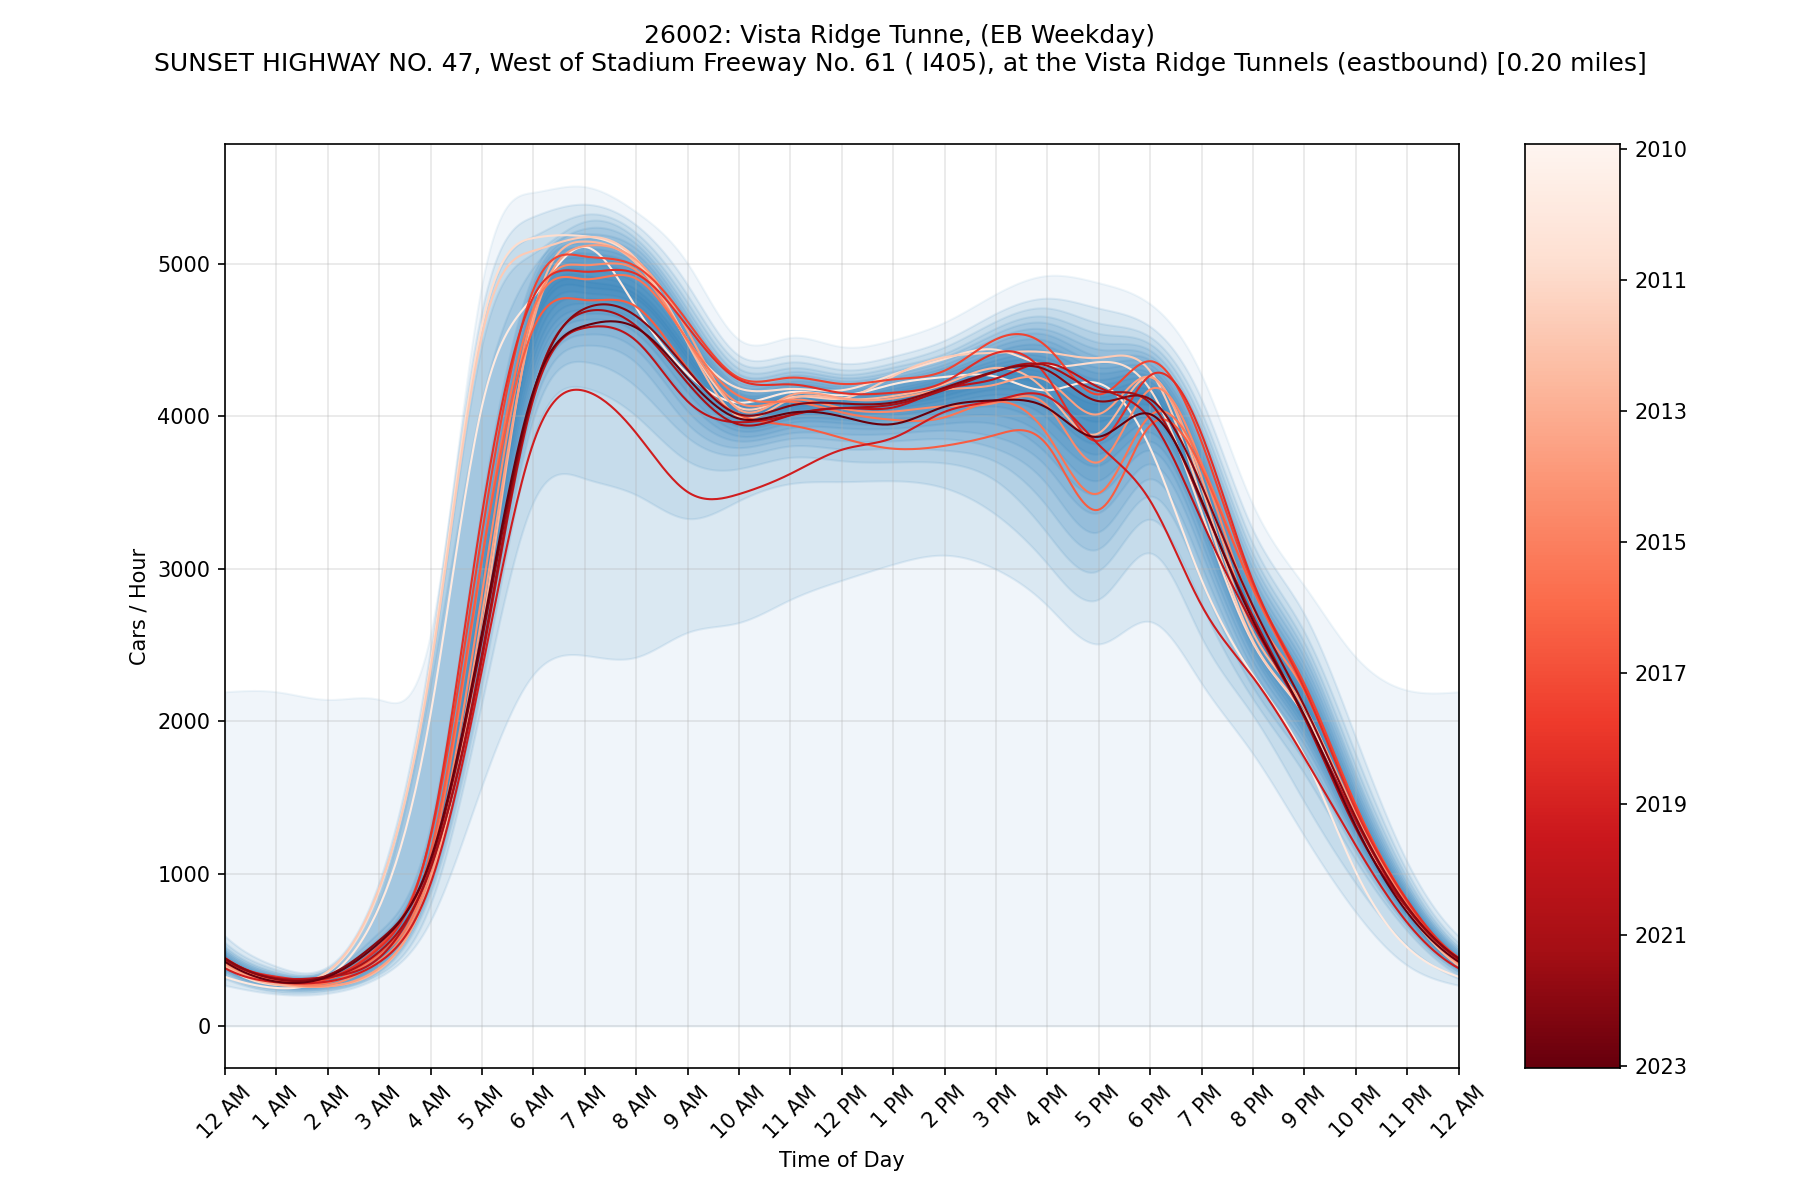
\includegraphics[width=\textwidth]{26002_Vista-Ridge-Tunne_EB_Weekday.png}
	\end{subfigure}
	\hfill
	\begin{subfigure}{0.45\textwidth}
		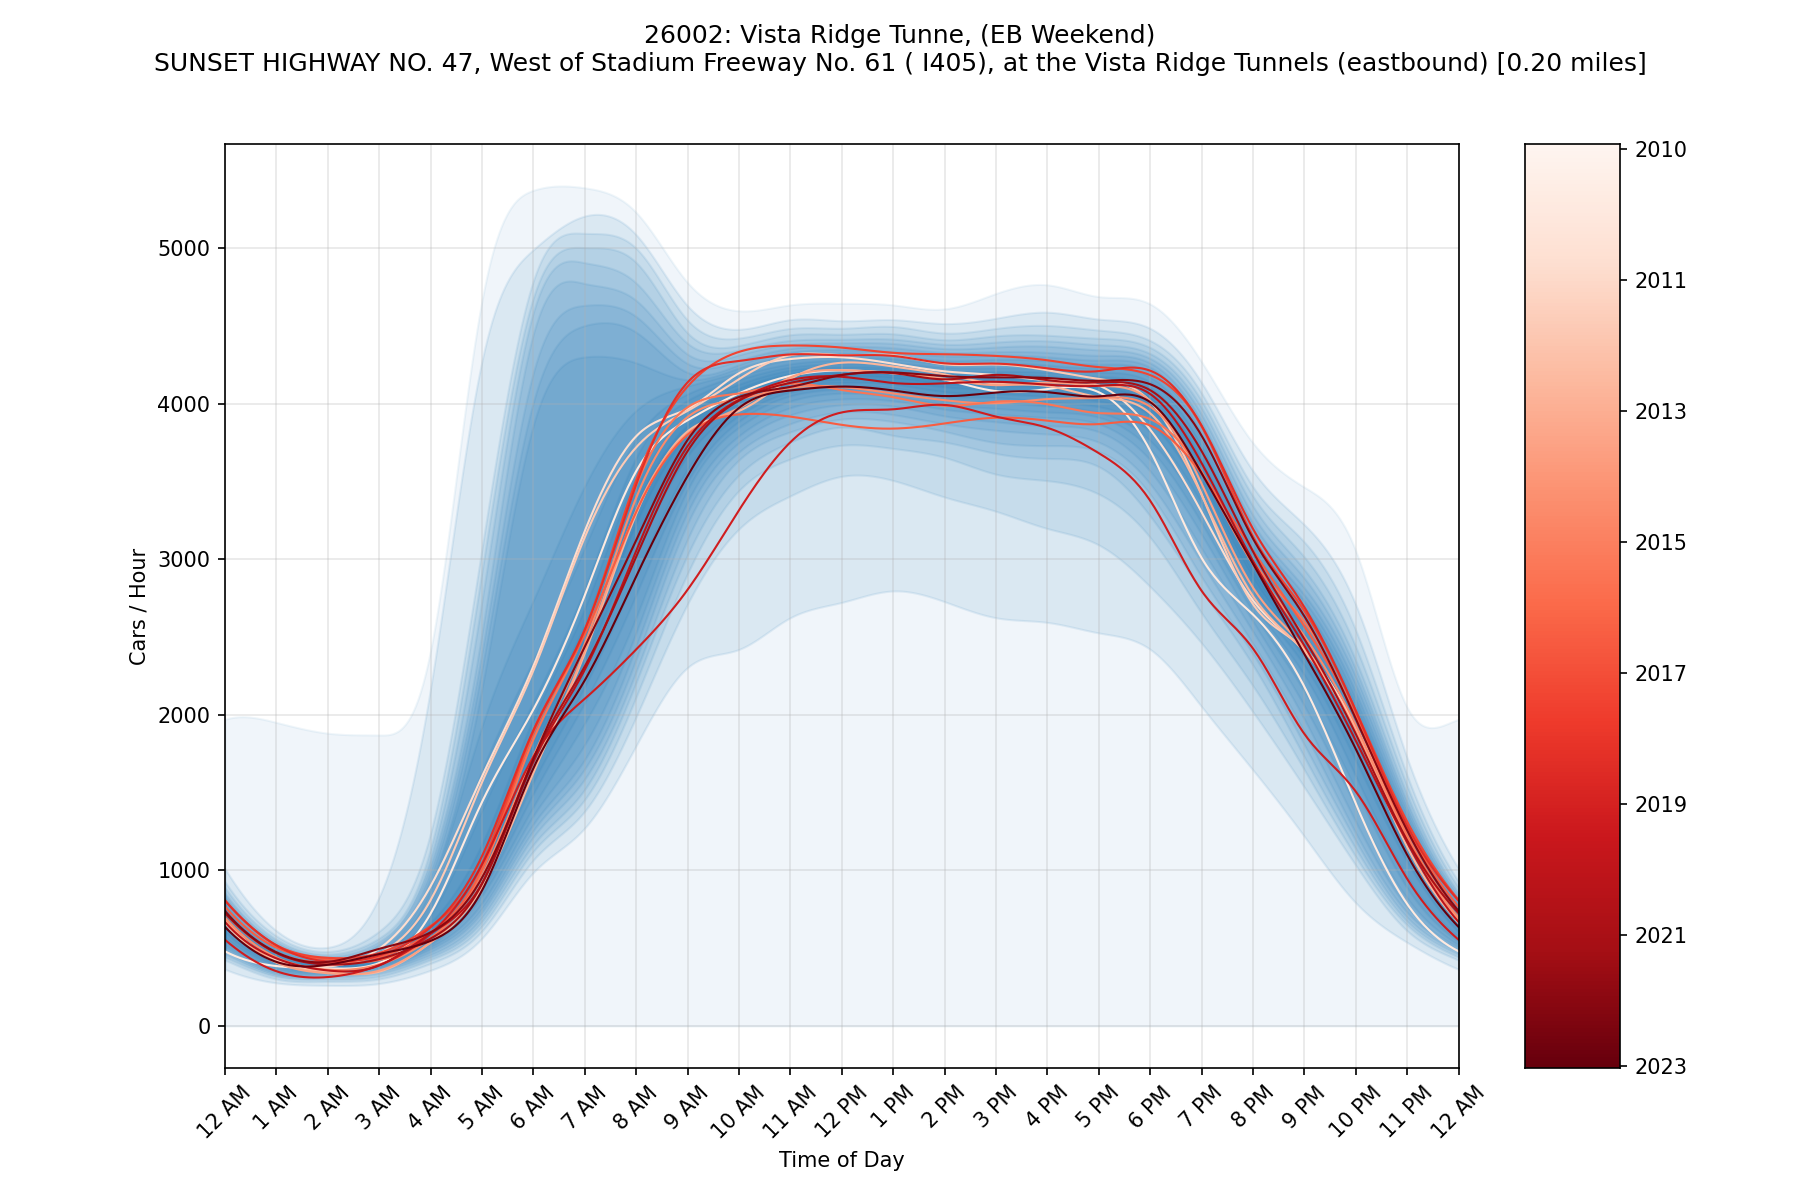
\includegraphics[width=\textwidth]{26002_Vista-Ridge-Tunne_EB_Weekend.png}
	\end{subfigure}

	\begin{subfigure}{0.45\textwidth}
		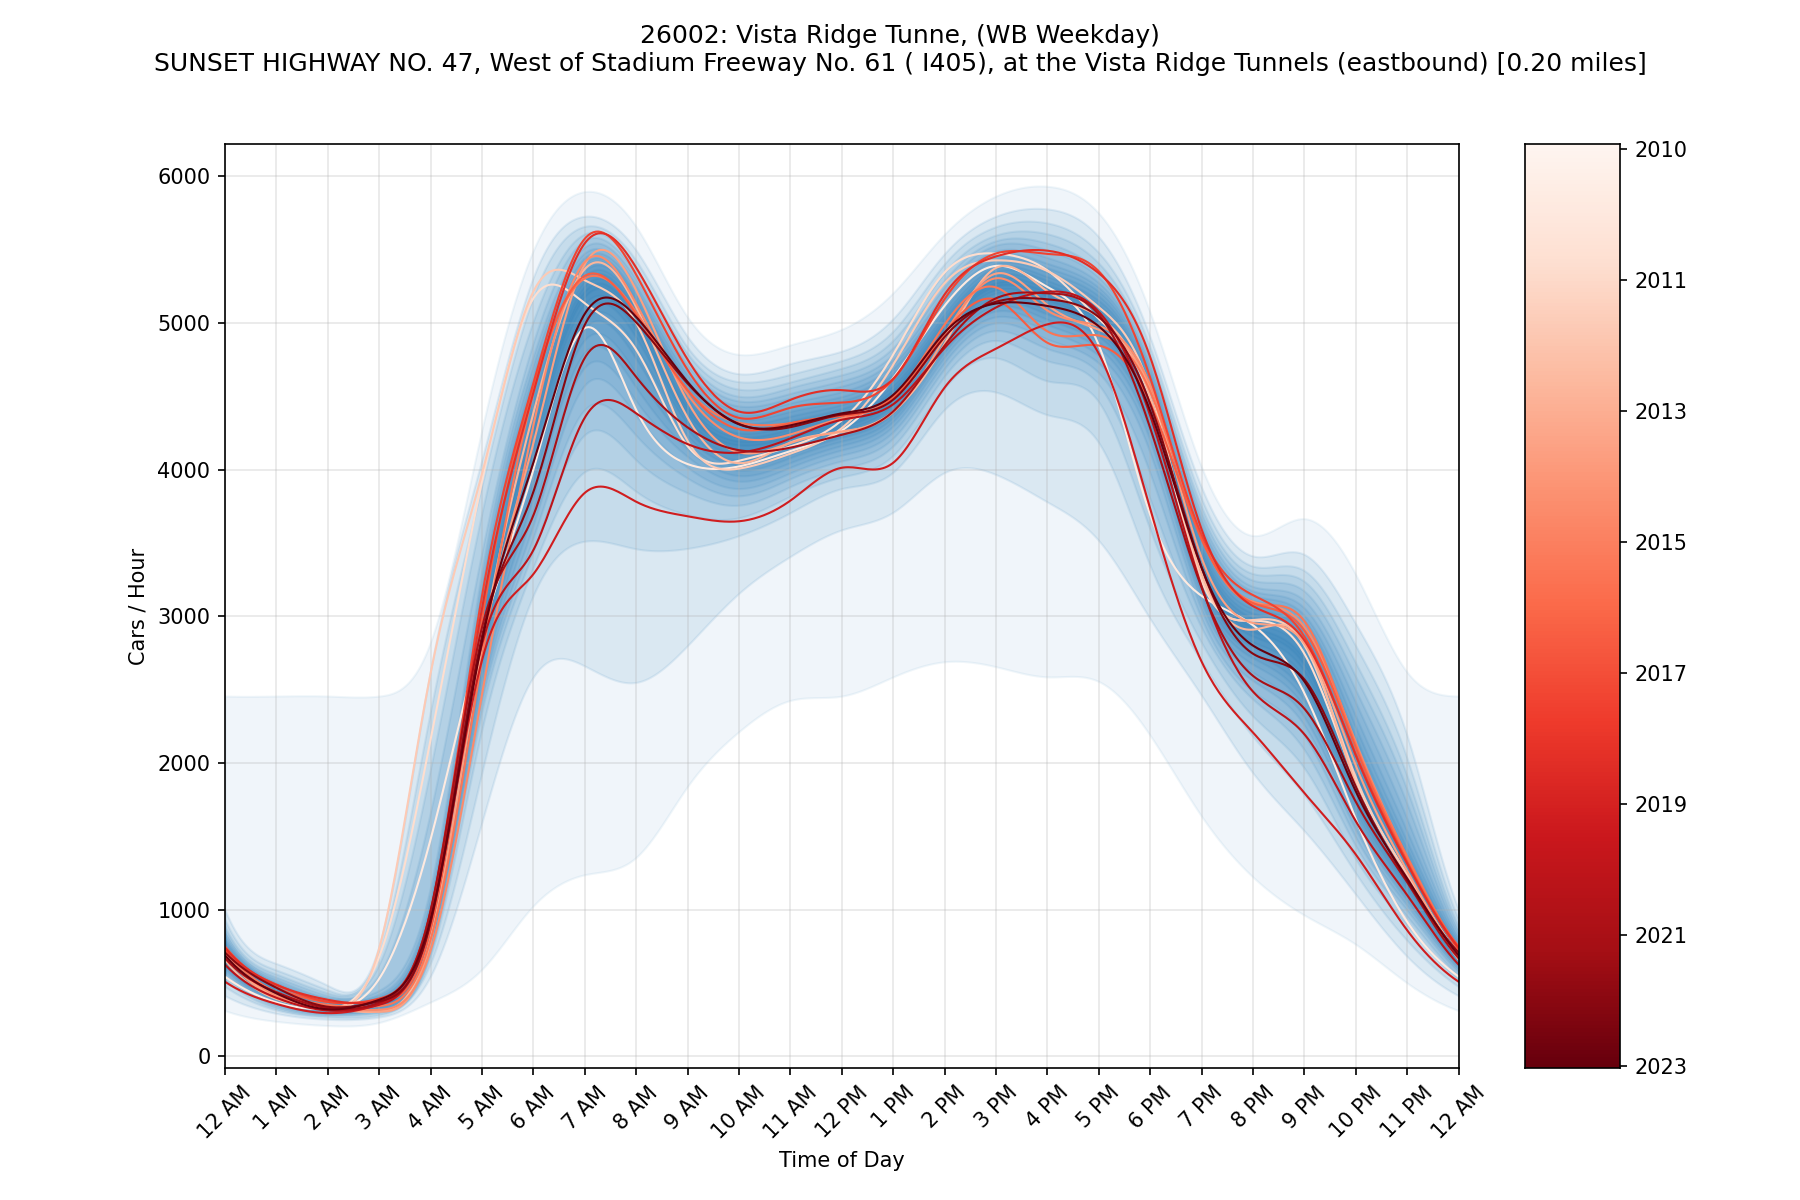
\includegraphics[width=\textwidth]{26002_Vista-Ridge-Tunne_WB_Weekday.png}
	\end{subfigure}
	\hfill
	\begin{subfigure}{0.45\textwidth}
		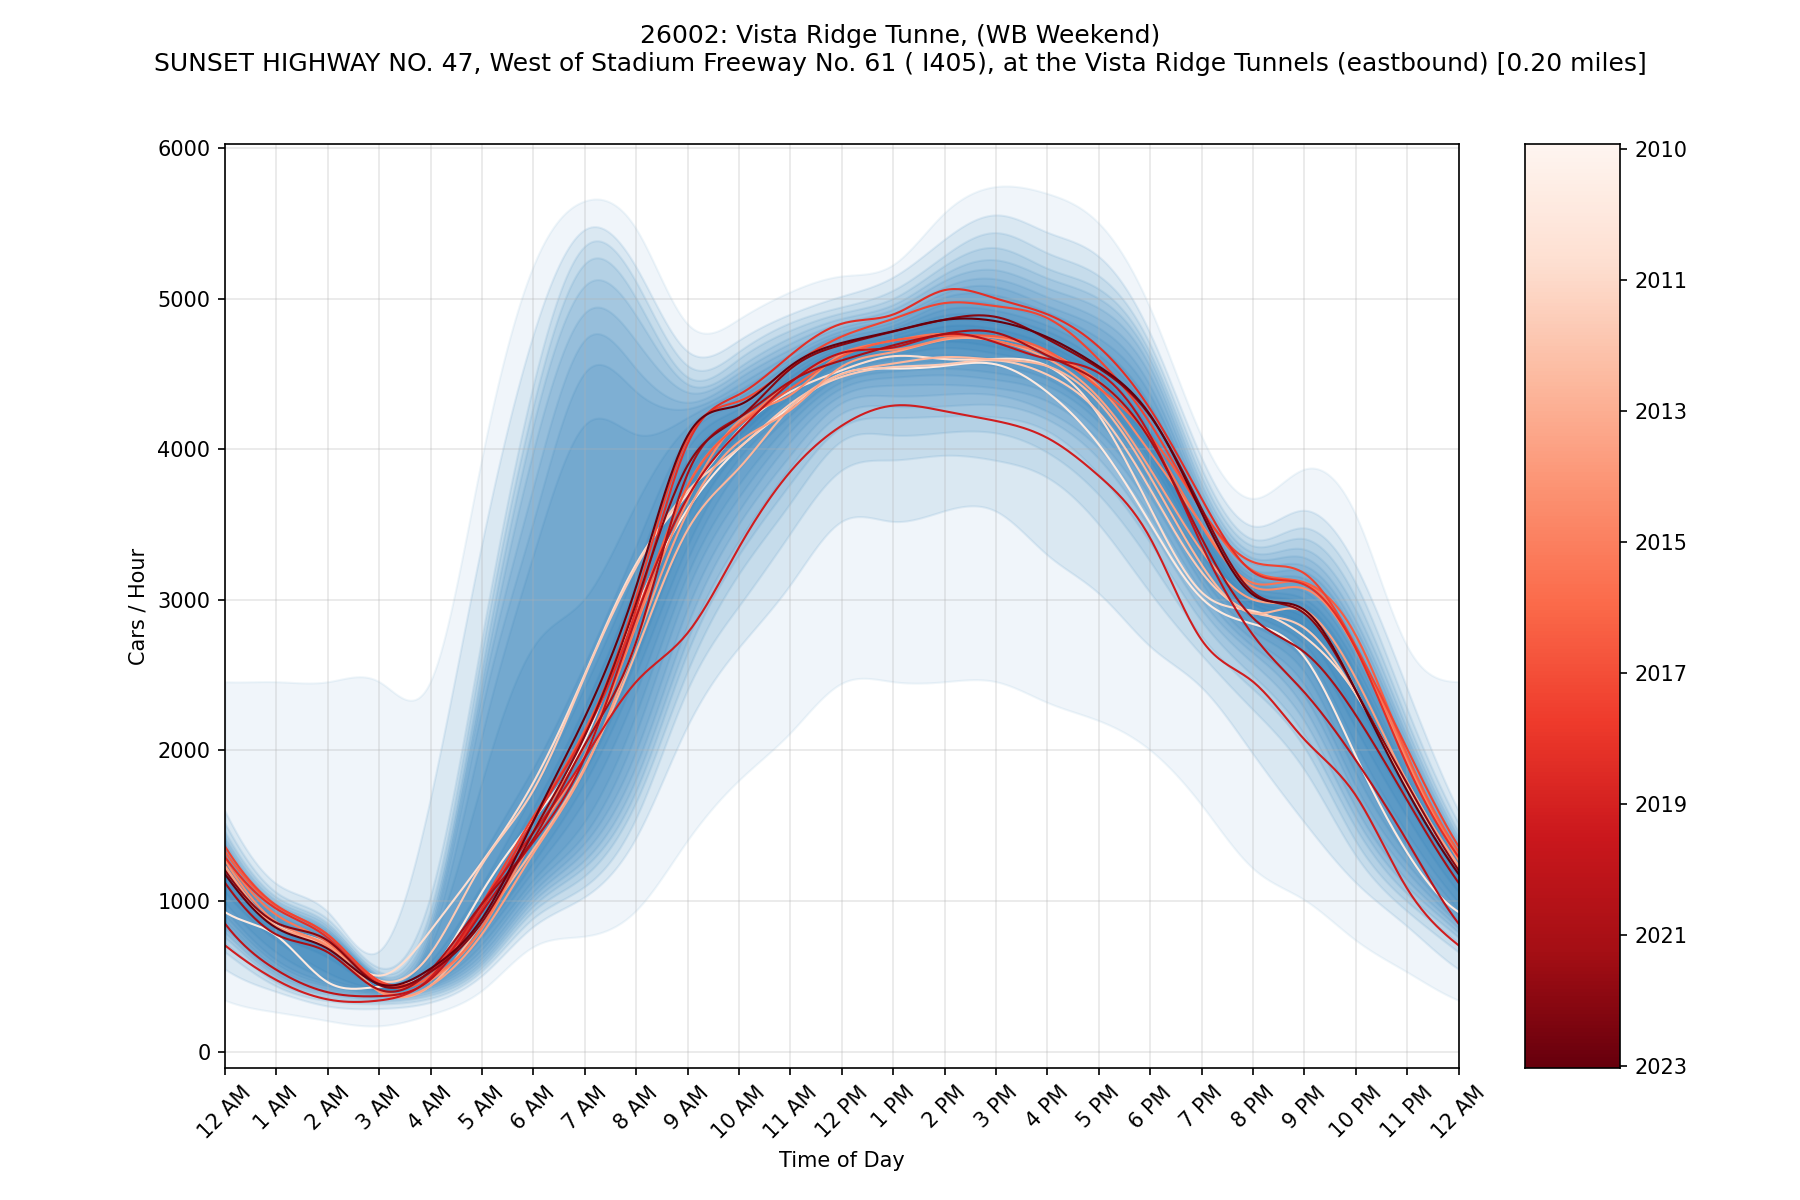
\includegraphics[width=\textwidth]{26002_Vista-Ridge-Tunne_WB_Weekend.png}
	\end{subfigure}
\end{figure}

\begin{figure}[htbp]
	\centering
	\begin{subfigure}{0.45\textwidth}
		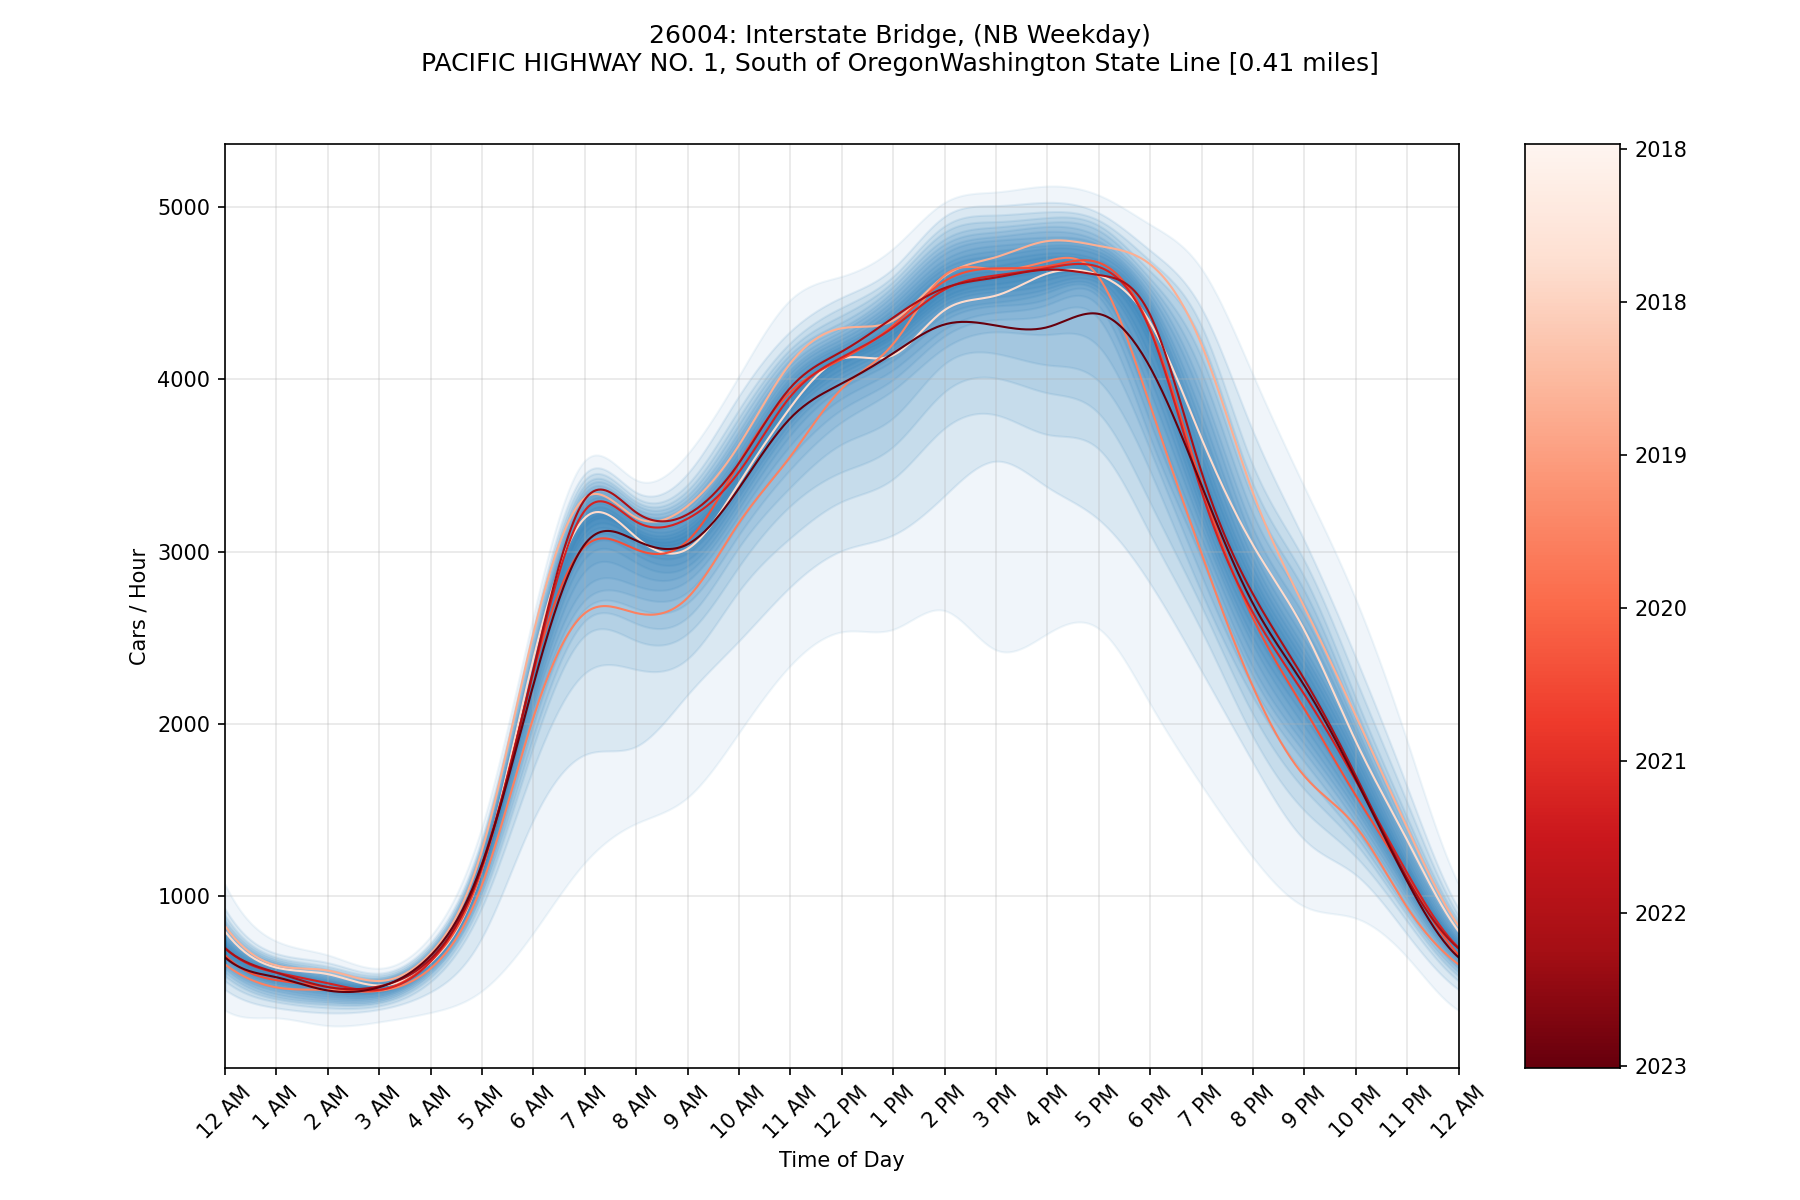
\includegraphics[width=\textwidth]{26004_Interstate-Bridge_NB_Weekday.png}
	\end{subfigure}
	\hfill
	\begin{subfigure}{0.45\textwidth}
		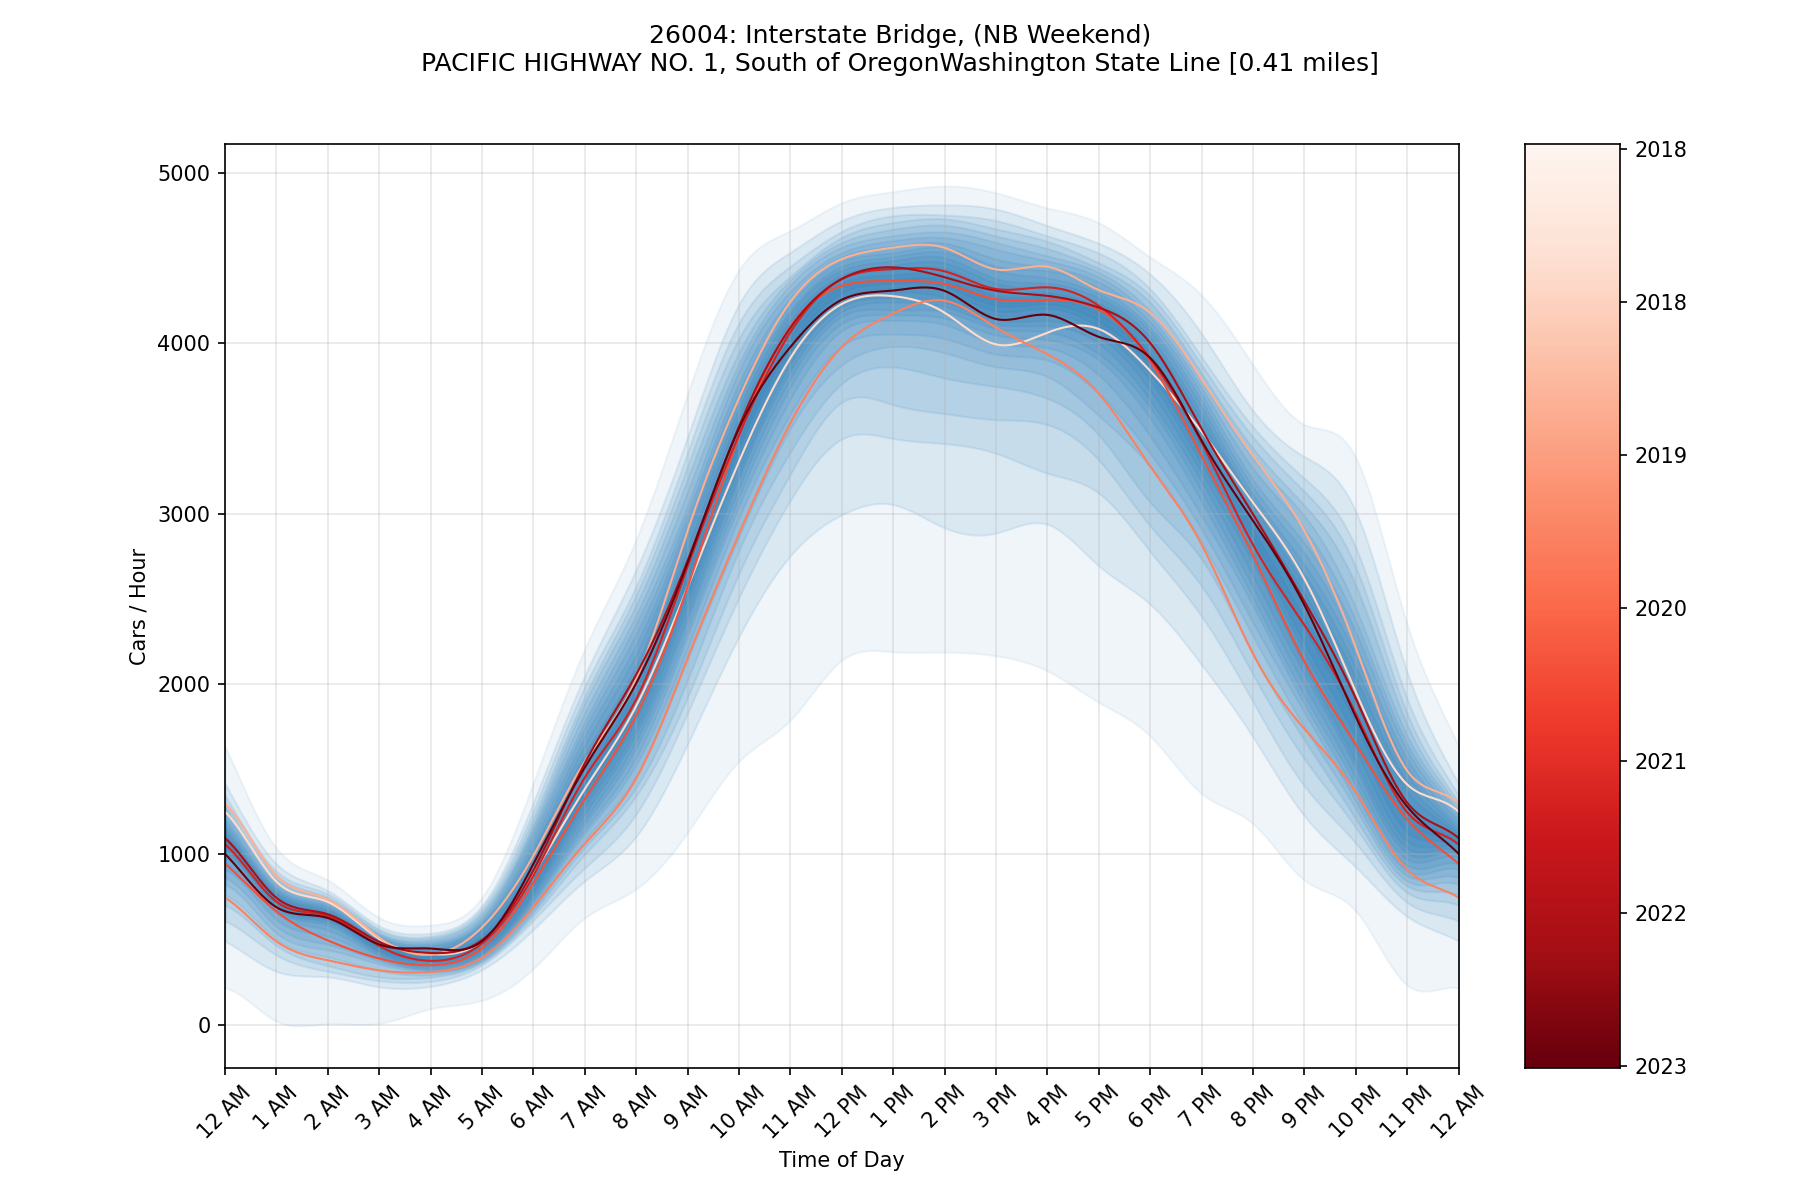
\includegraphics[width=\textwidth]{26004_Interstate-Bridge_NB_Weekend.png}
	\end{subfigure}

	\begin{subfigure}{0.45\textwidth}
		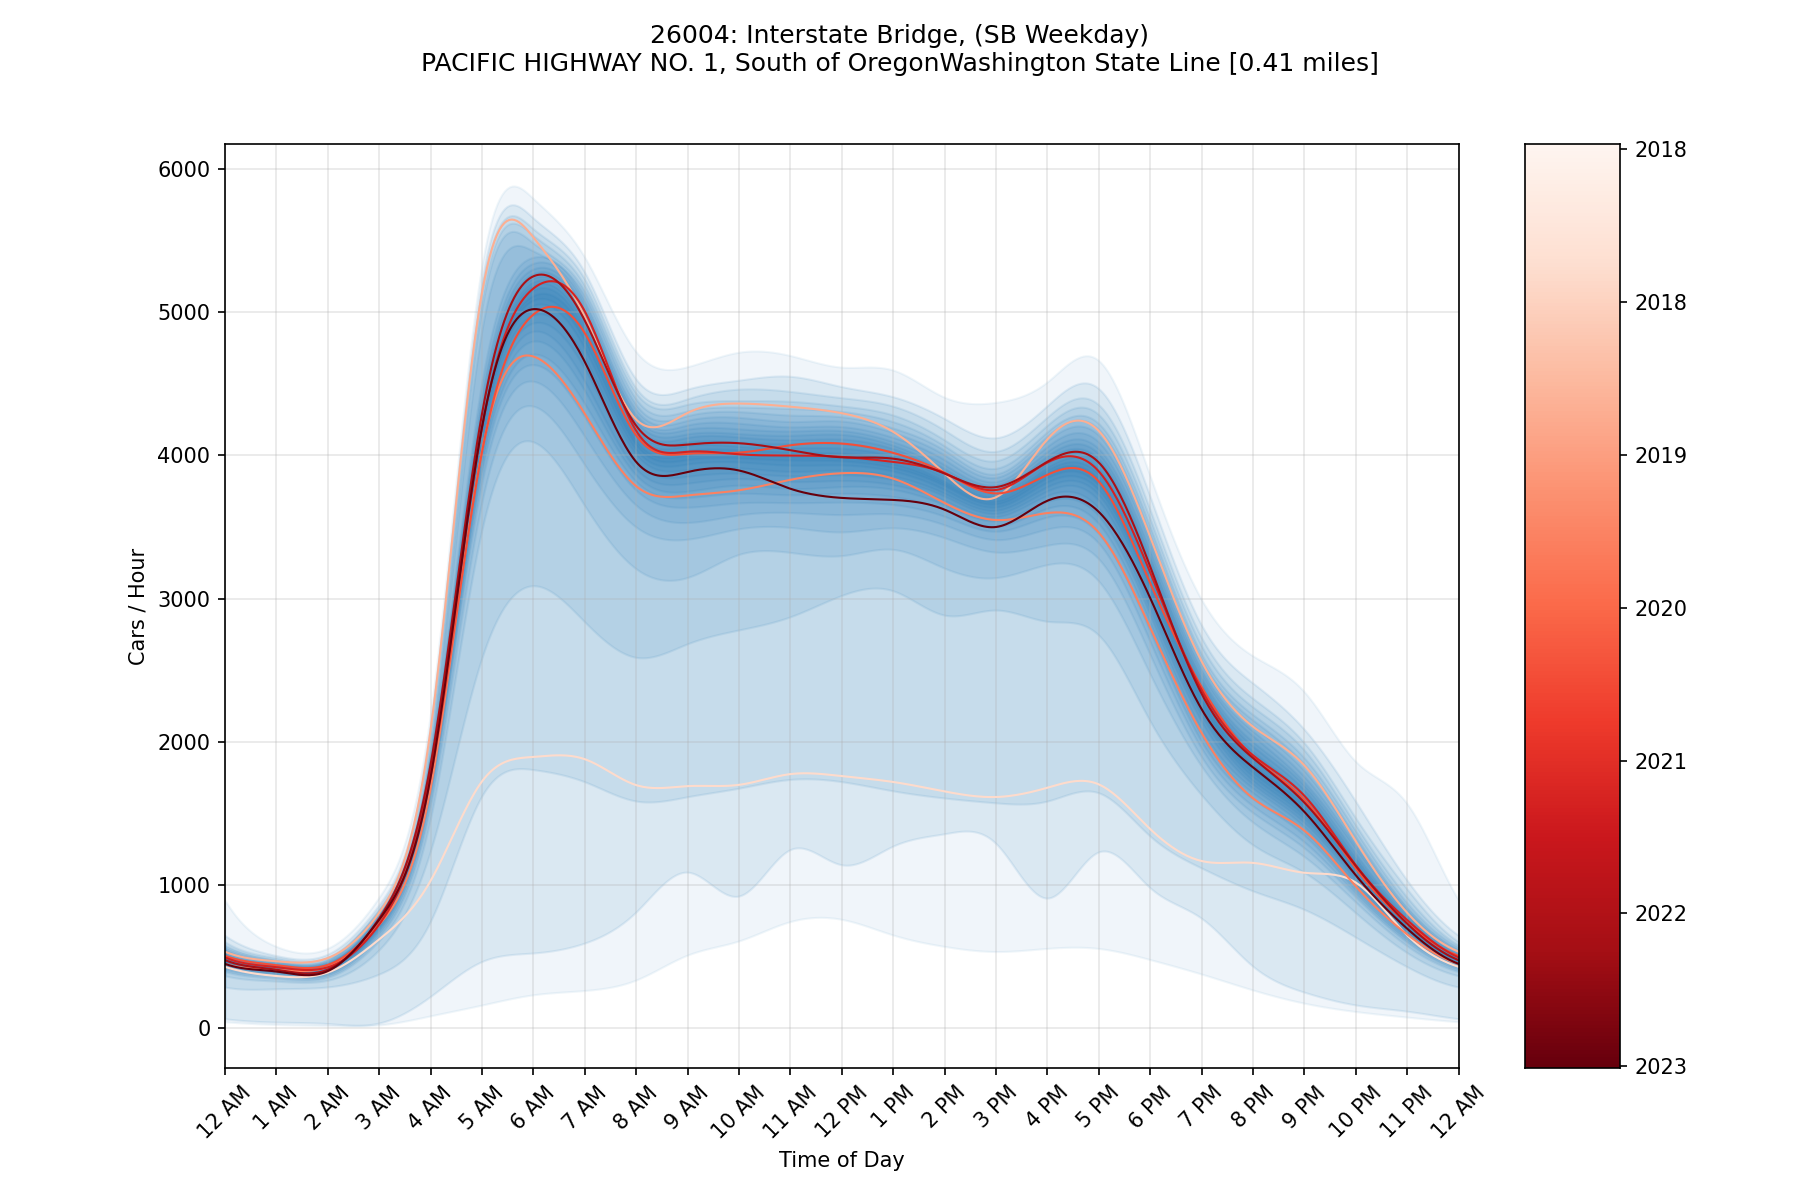
\includegraphics[width=\textwidth]{26004_Interstate-Bridge_SB_Weekday.png}
	\end{subfigure}
	\hfill
	\begin{subfigure}{0.45\textwidth}
		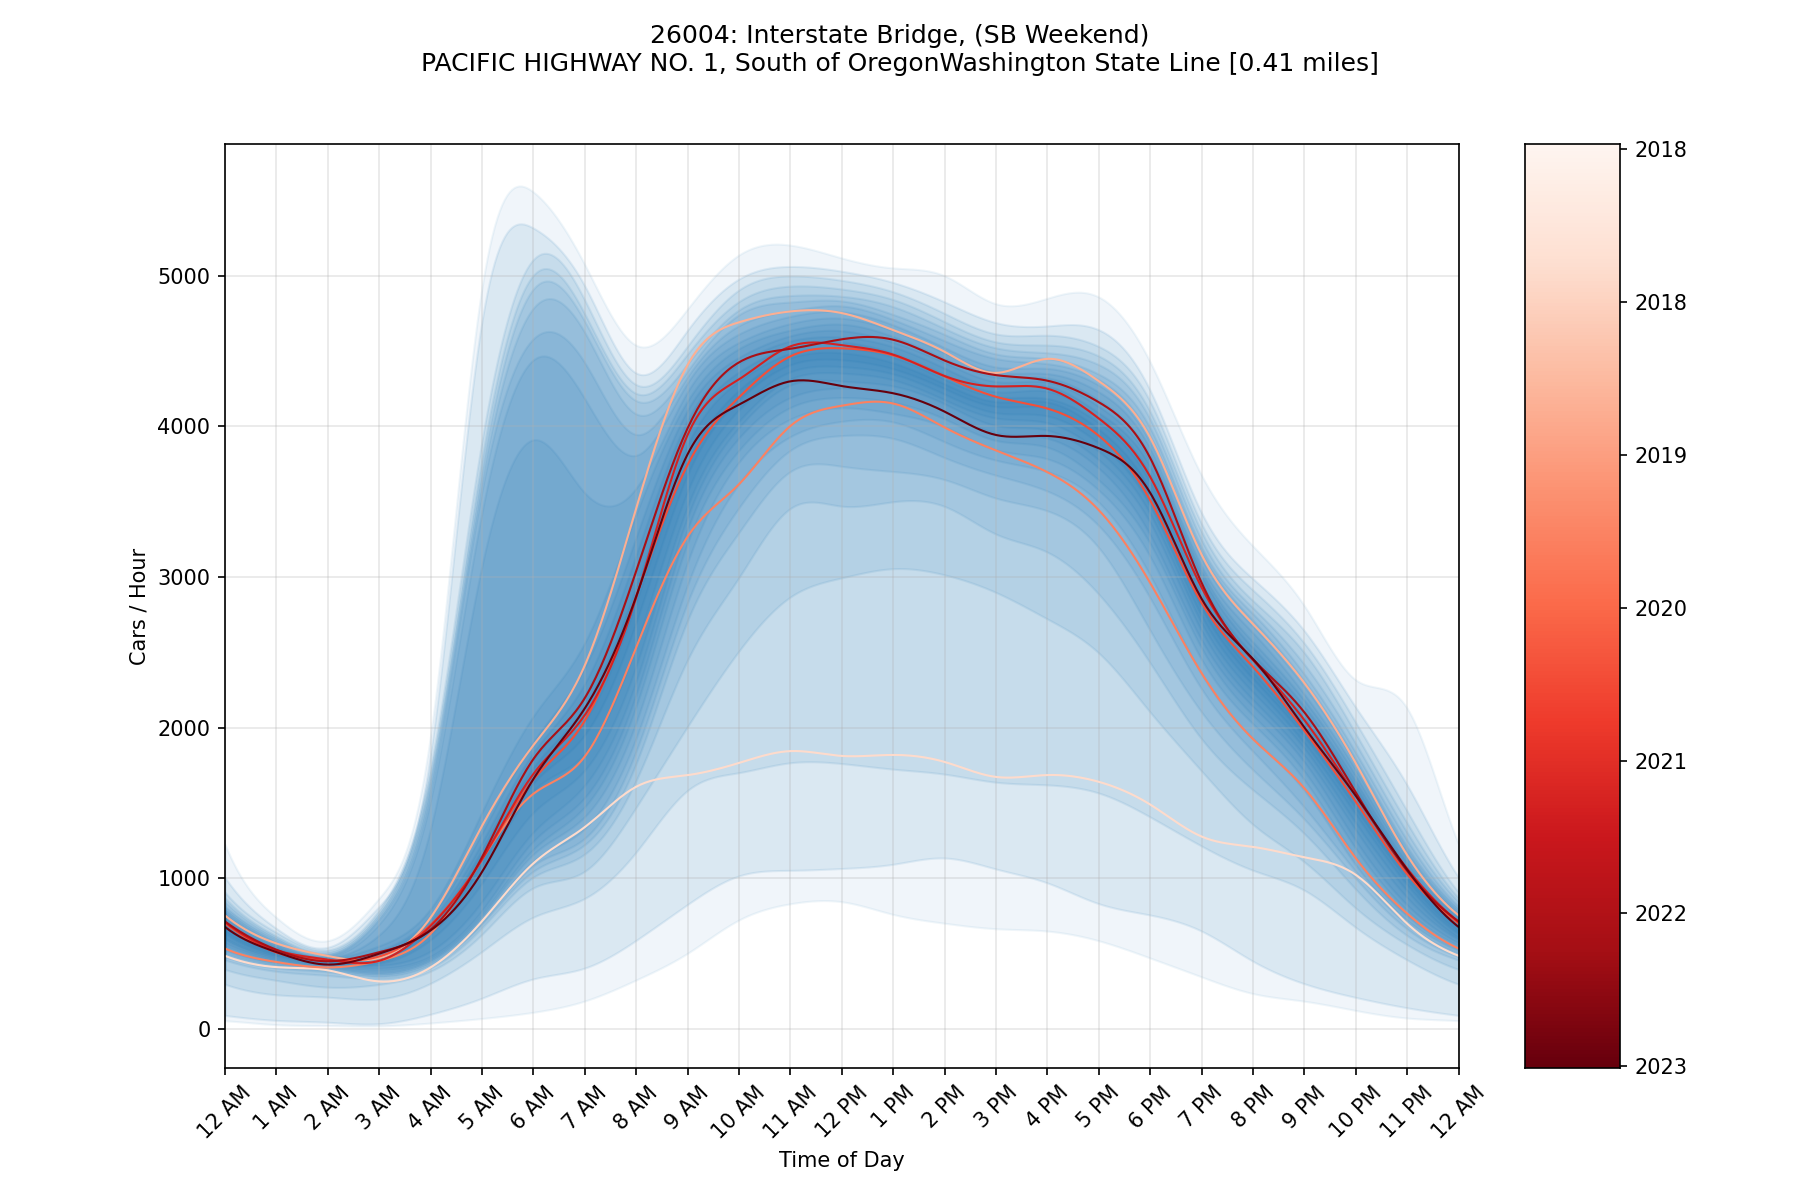
\includegraphics[width=\textwidth]{26004_Interstate-Bridge_SB_Weekend.png}
	\end{subfigure}
\end{figure}

\begin{figure}[htbp]
	\centering
	\begin{subfigure}{0.45\textwidth}
		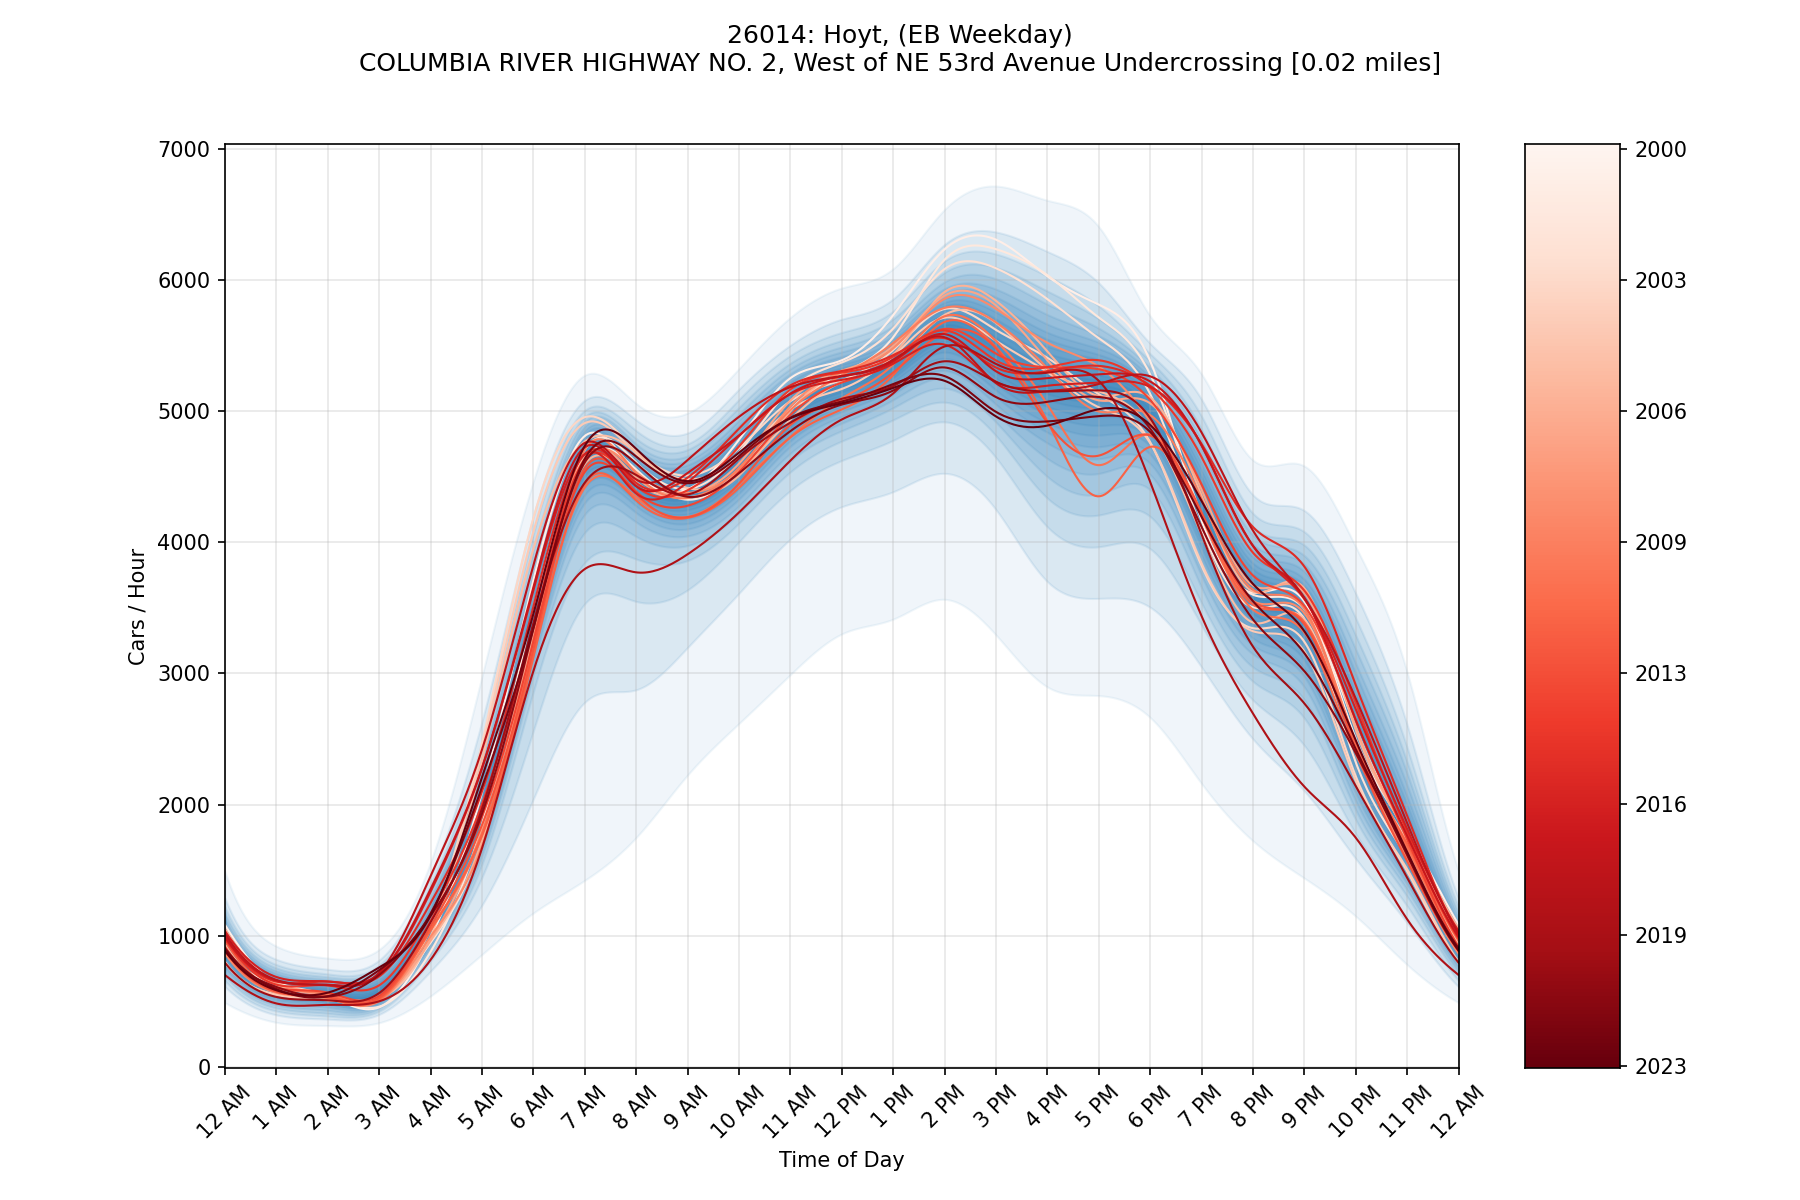
\includegraphics[width=\textwidth]{26014_Hoyt_EB_Weekday.png}
	\end{subfigure}
	\hfill
	\begin{subfigure}{0.45\textwidth}
		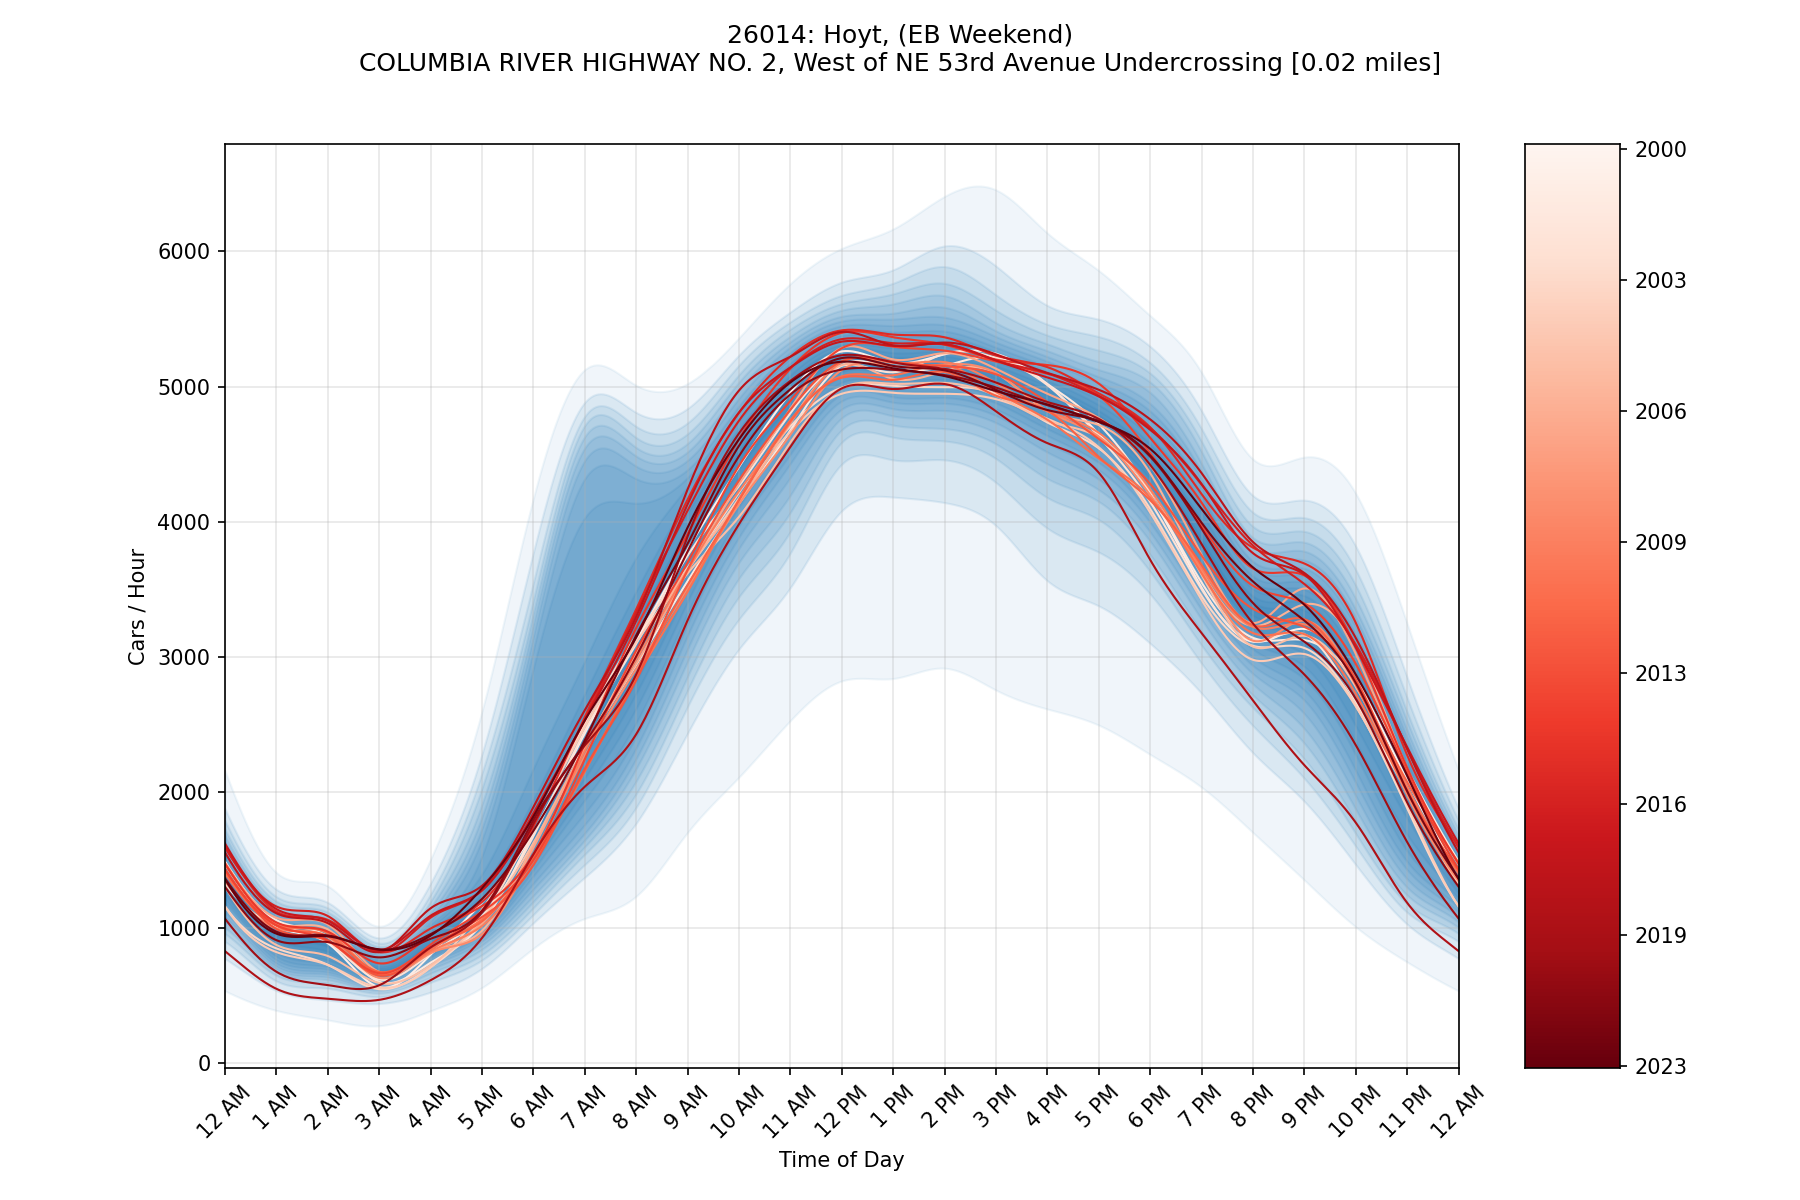
\includegraphics[width=\textwidth]{26014_Hoyt_EB_Weekend.png}
	\end{subfigure}

	\begin{subfigure}{0.45\textwidth}
		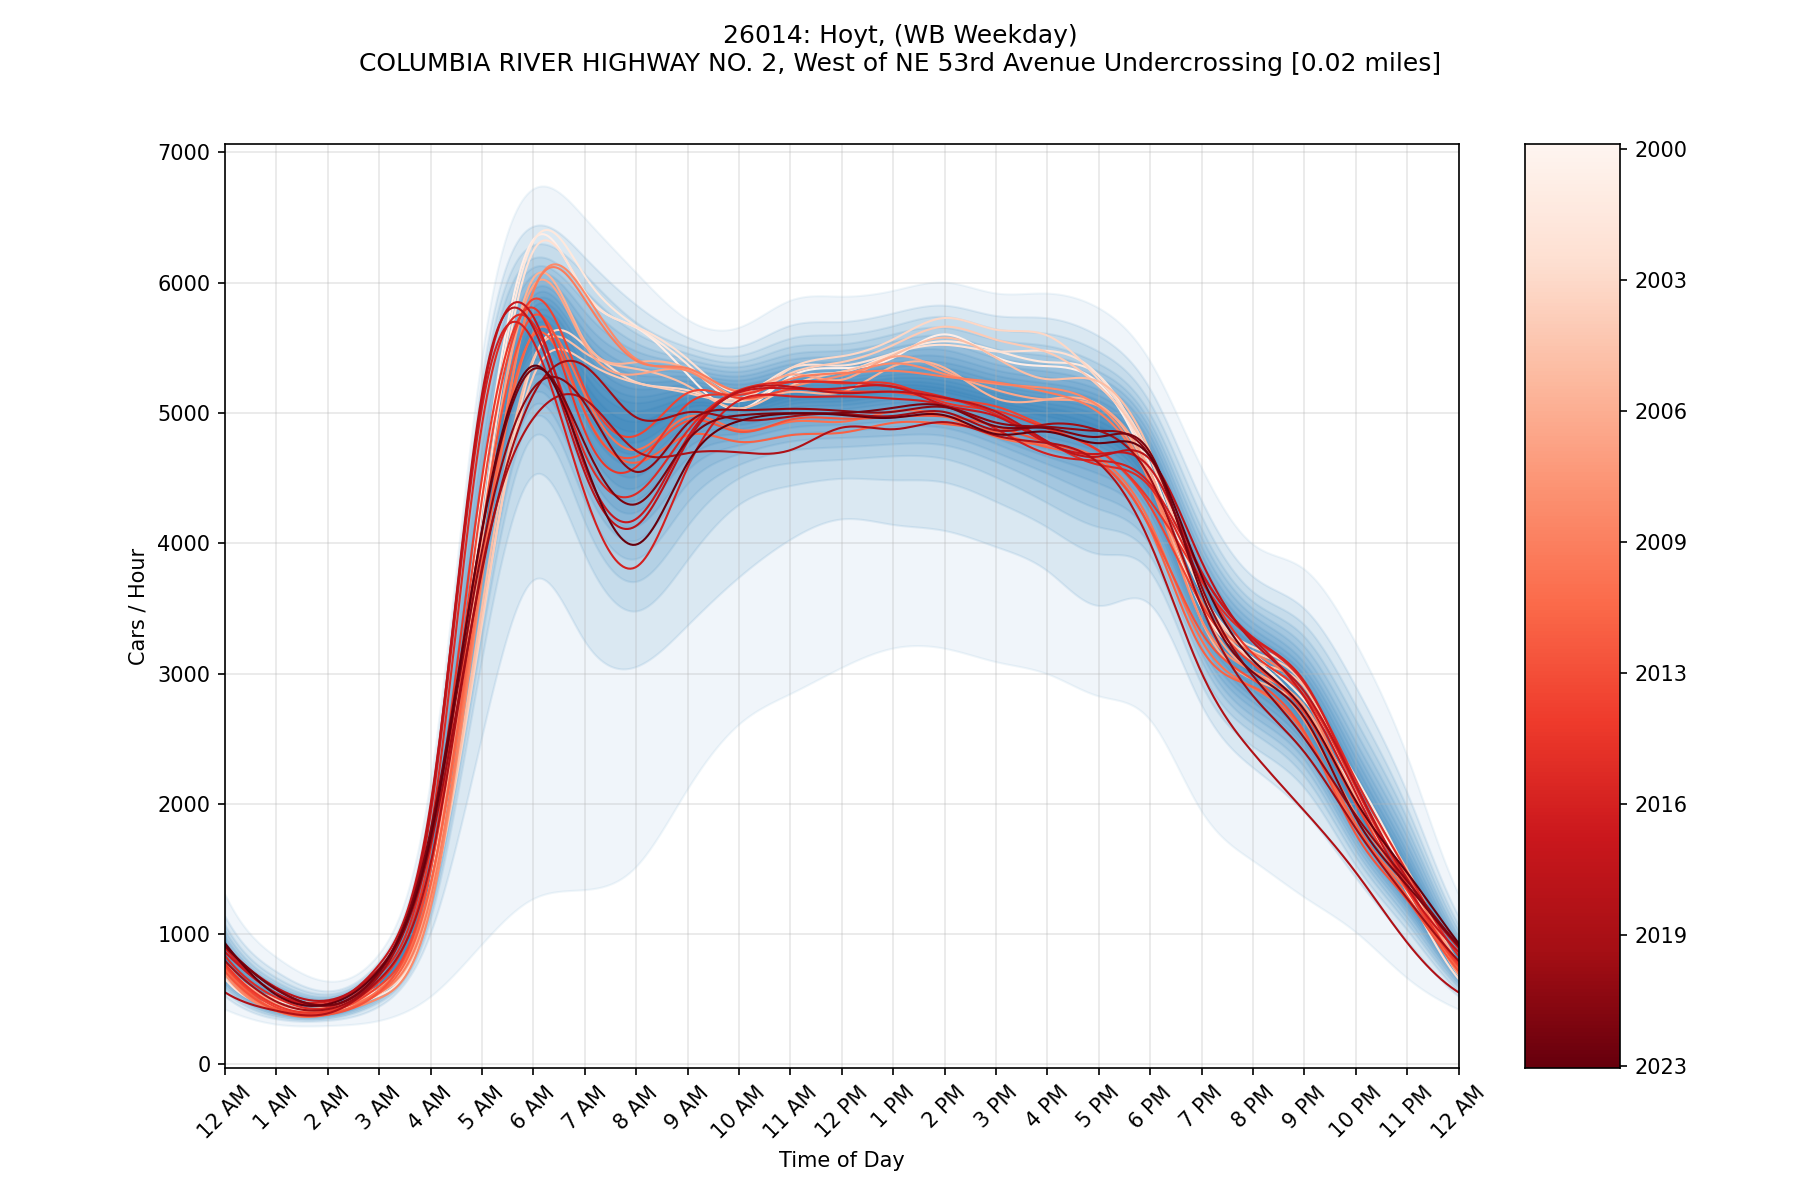
\includegraphics[width=\textwidth]{26014_Hoyt_WB_Weekday.png}
	\end{subfigure}
	\hfill
	\begin{subfigure}{0.45\textwidth}
		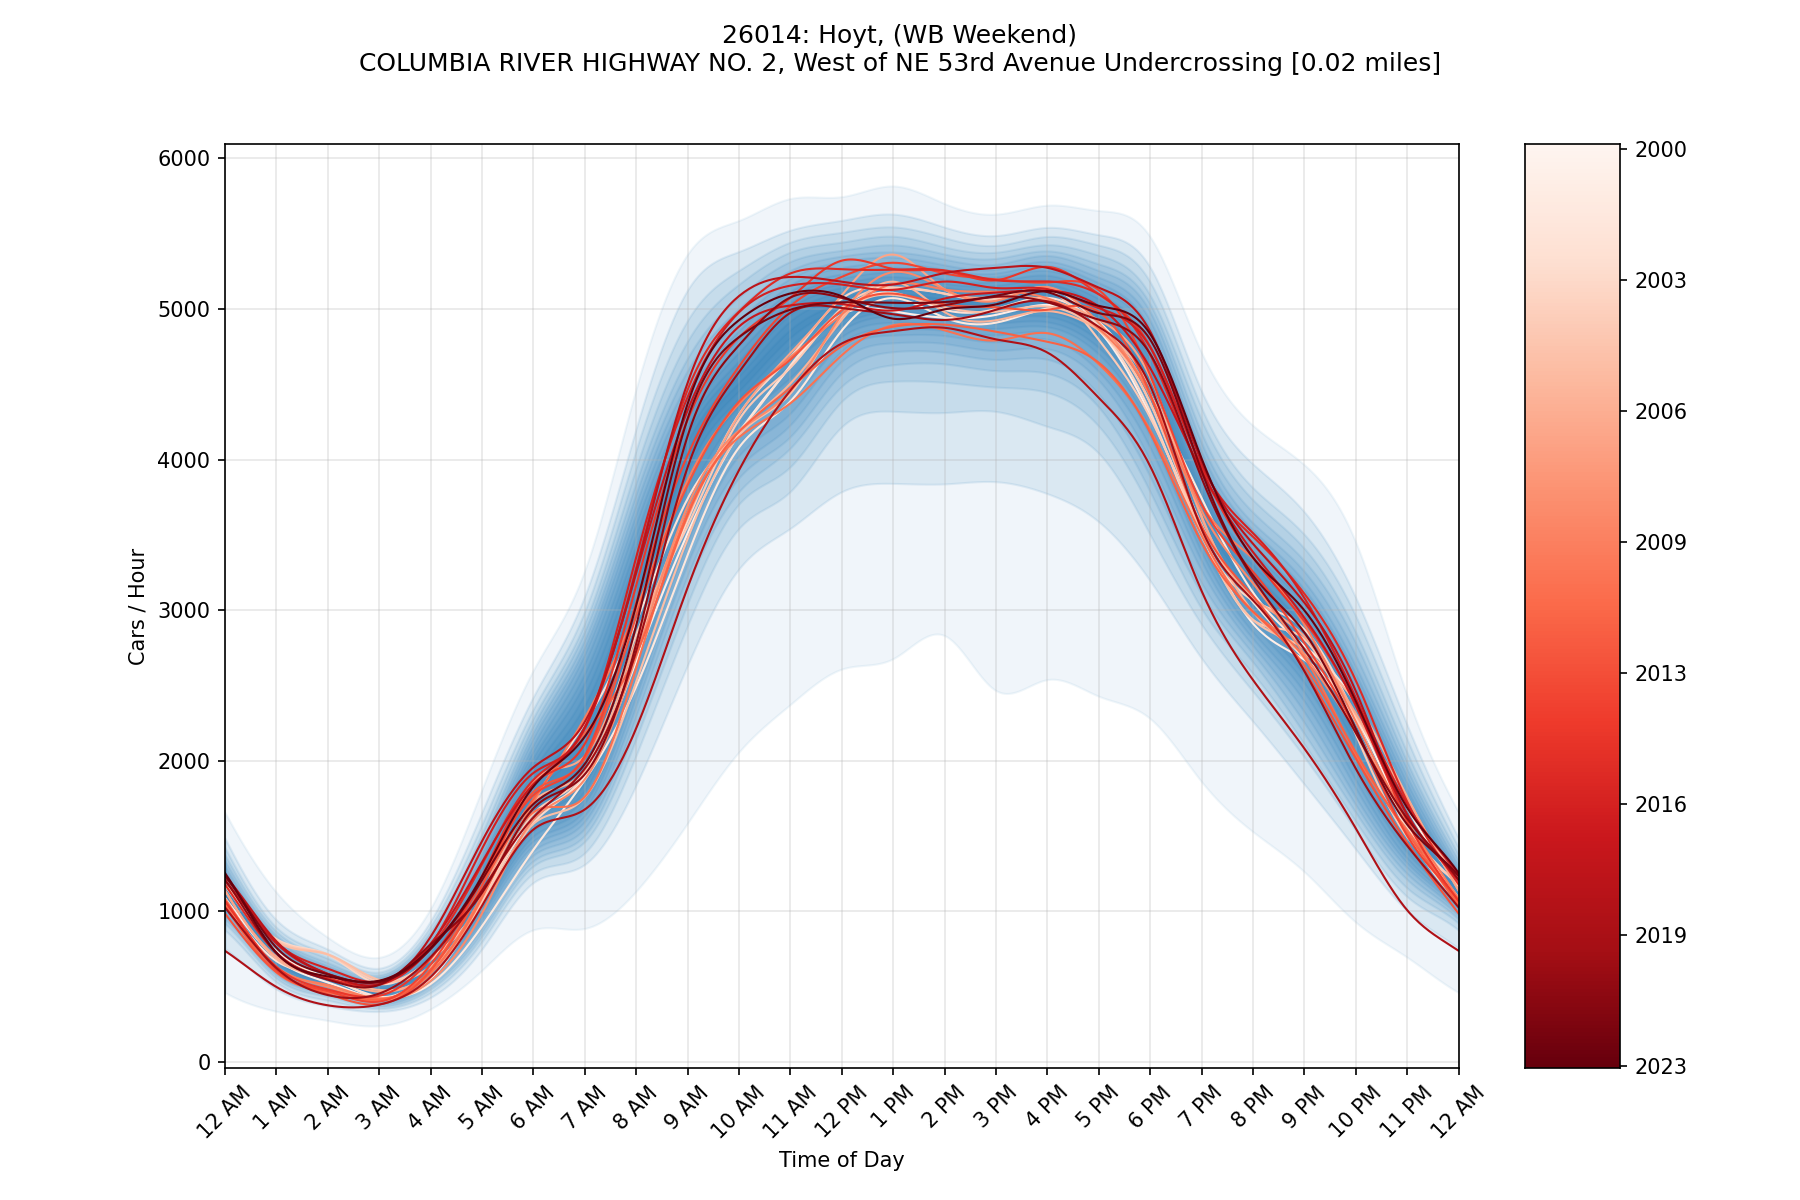
\includegraphics[width=\textwidth]{26014_Hoyt_WB_Weekend.png}
	\end{subfigure}
\end{figure}

\begin{figure}[htbp]
	\centering
	\begin{subfigure}{0.45\textwidth}
		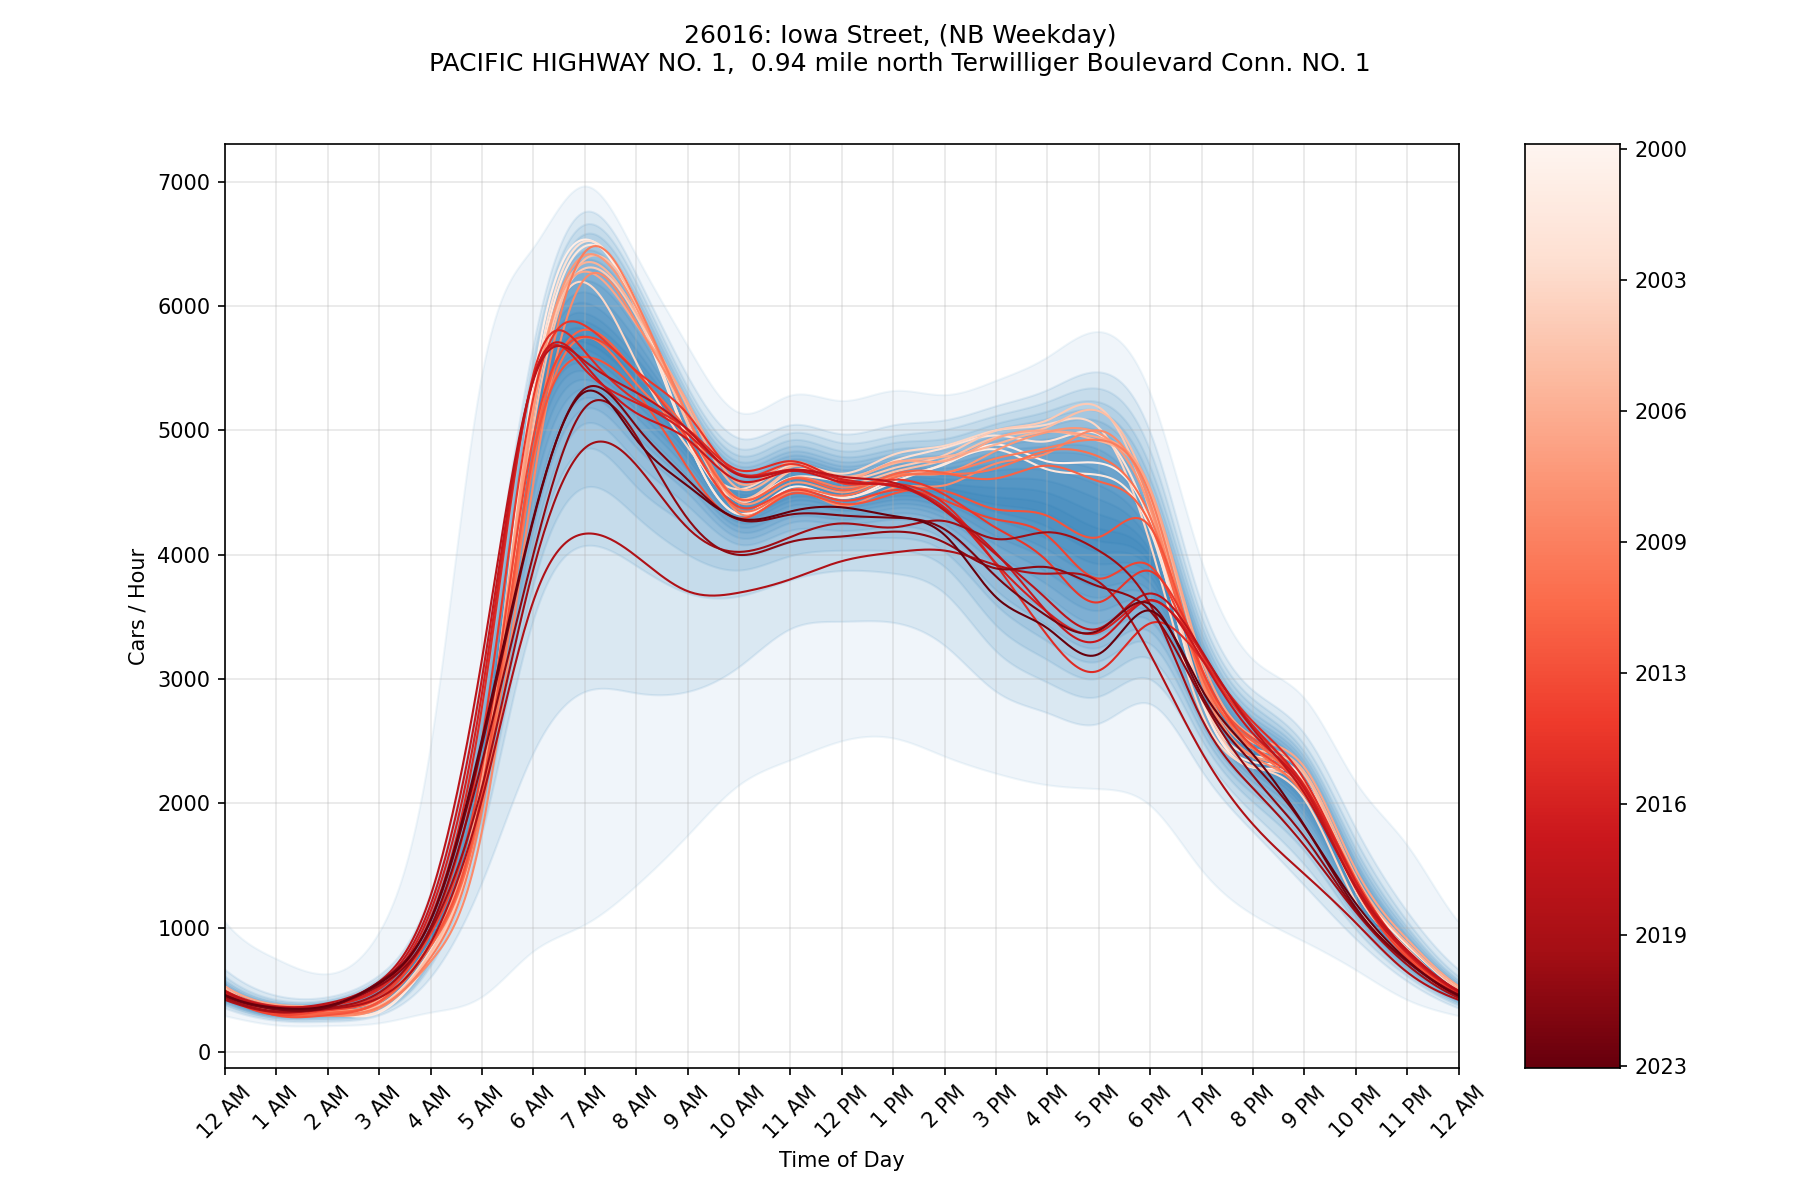
\includegraphics[width=\textwidth]{26016_Iowa-Street_NB_Weekday.png}
	\end{subfigure}
	\hfill
	\begin{subfigure}{0.45\textwidth}
		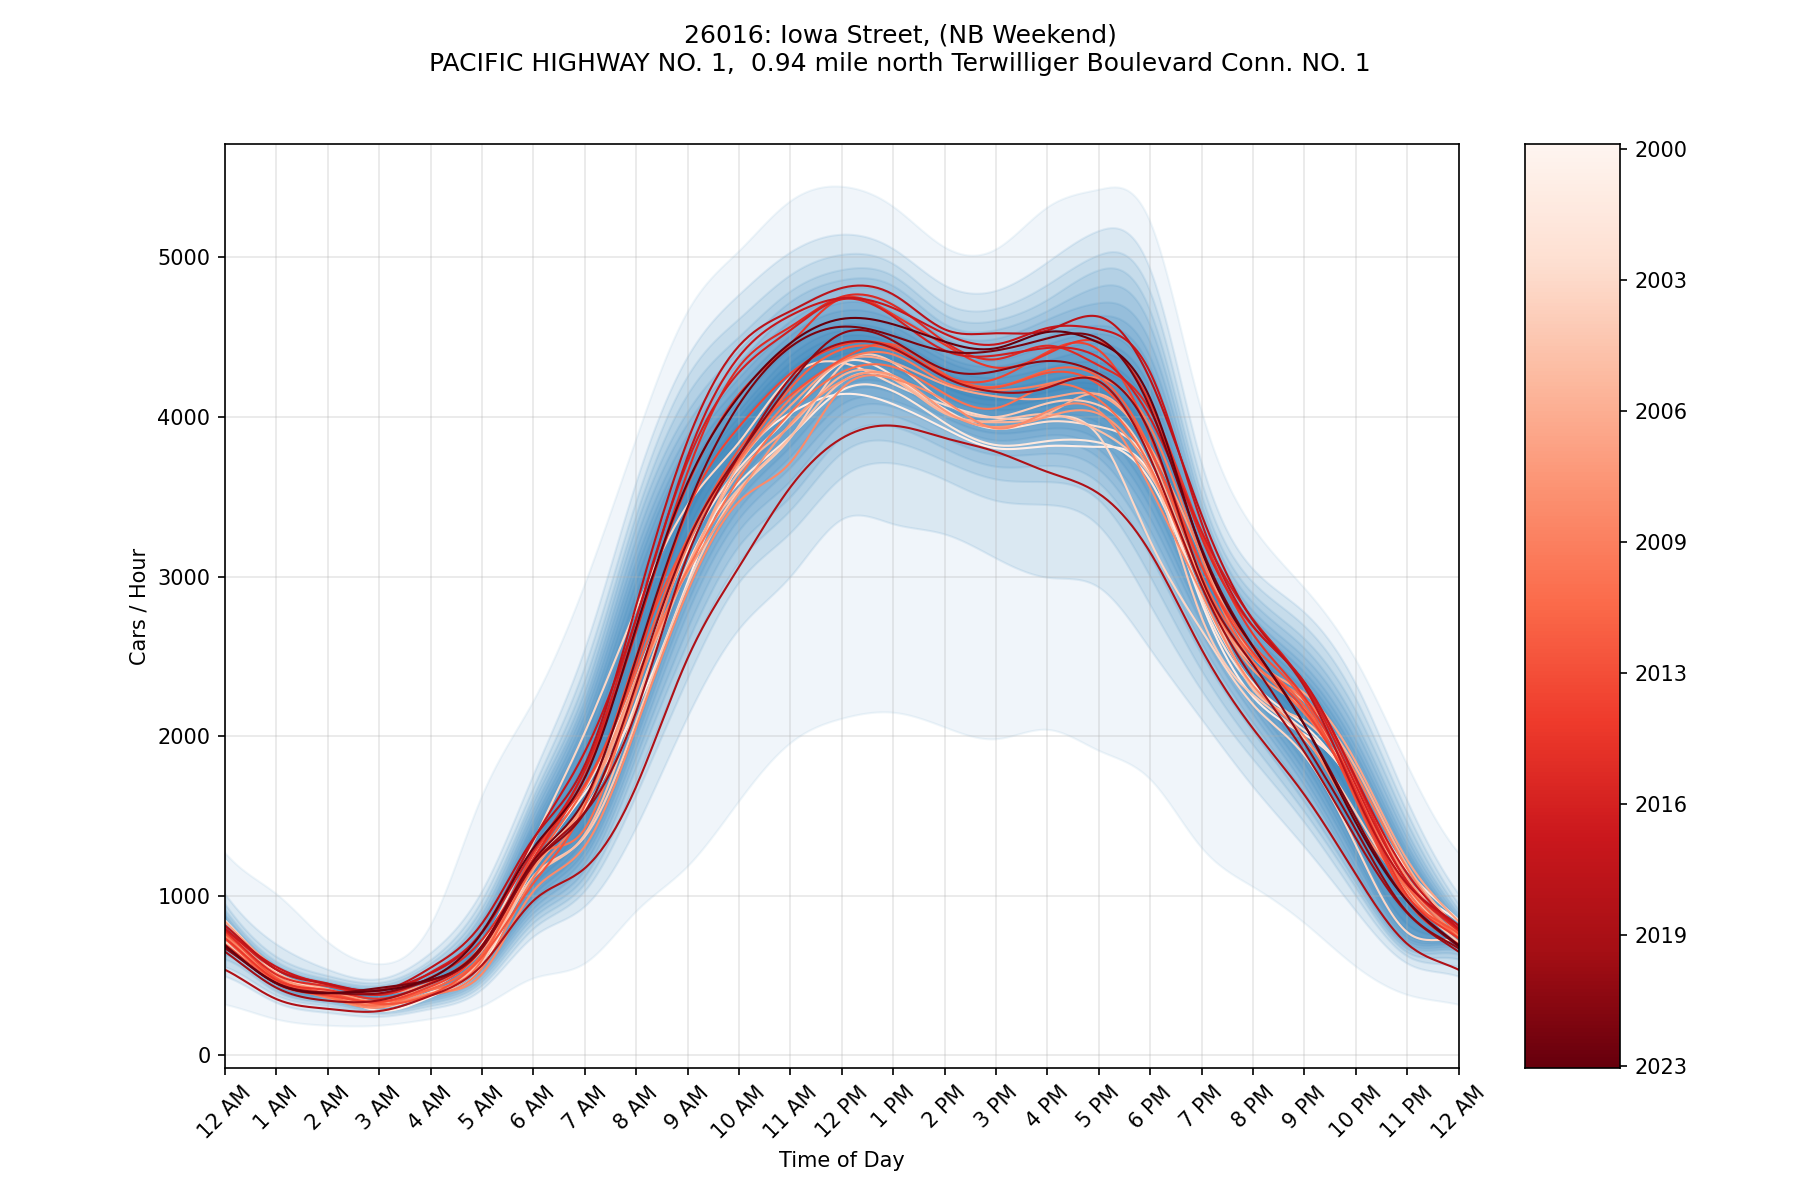
\includegraphics[width=\textwidth]{26016_Iowa-Street_NB_Weekend.png}
	\end{subfigure}

	\begin{subfigure}{0.45\textwidth}
		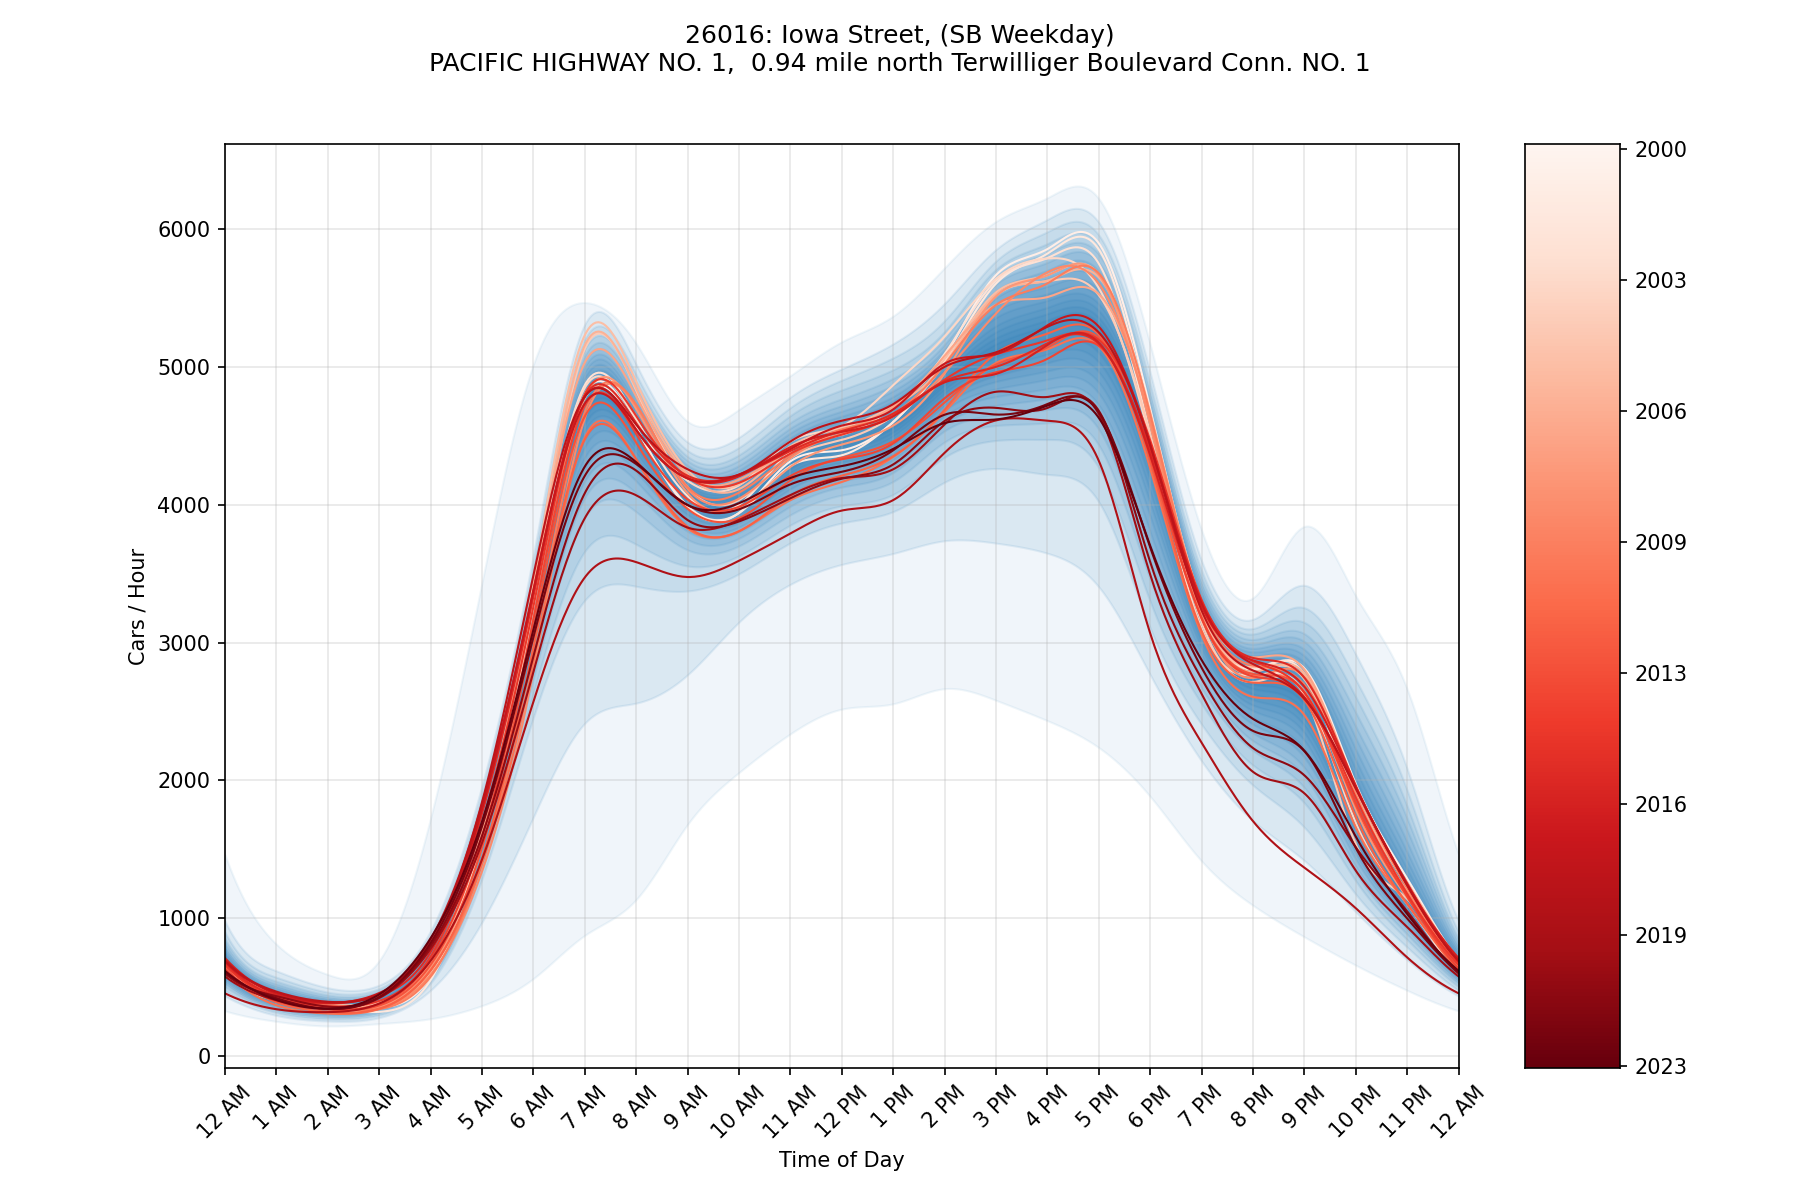
\includegraphics[width=\textwidth]{26016_Iowa-Street_SB_Weekday.png}
	\end{subfigure}
	\hfill
	\begin{subfigure}{0.45\textwidth}
		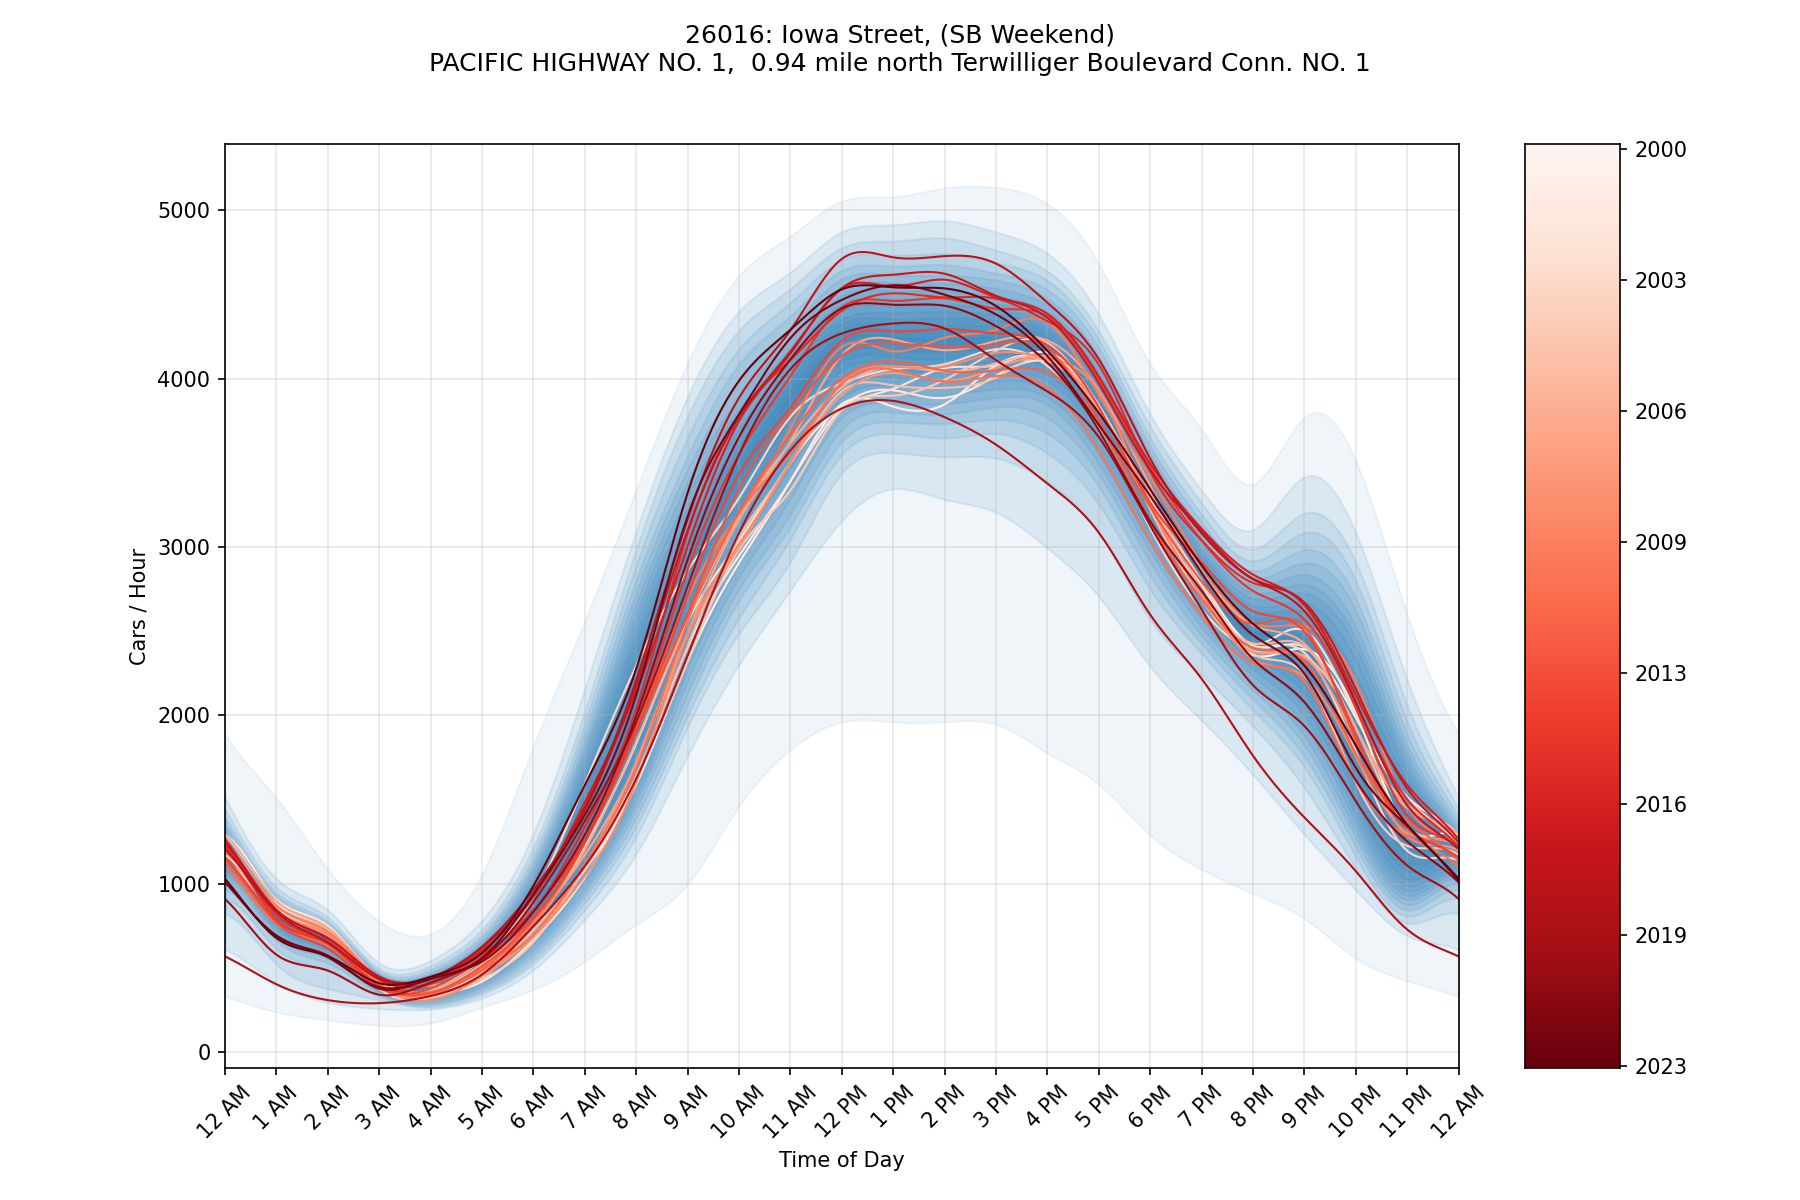
\includegraphics[width=\textwidth]{26016_Iowa-Street_SB_Weekend.png}
	\end{subfigure}
\end{figure}

\begin{figure}[htbp]
	\centering
	\begin{subfigure}{0.45\textwidth}
		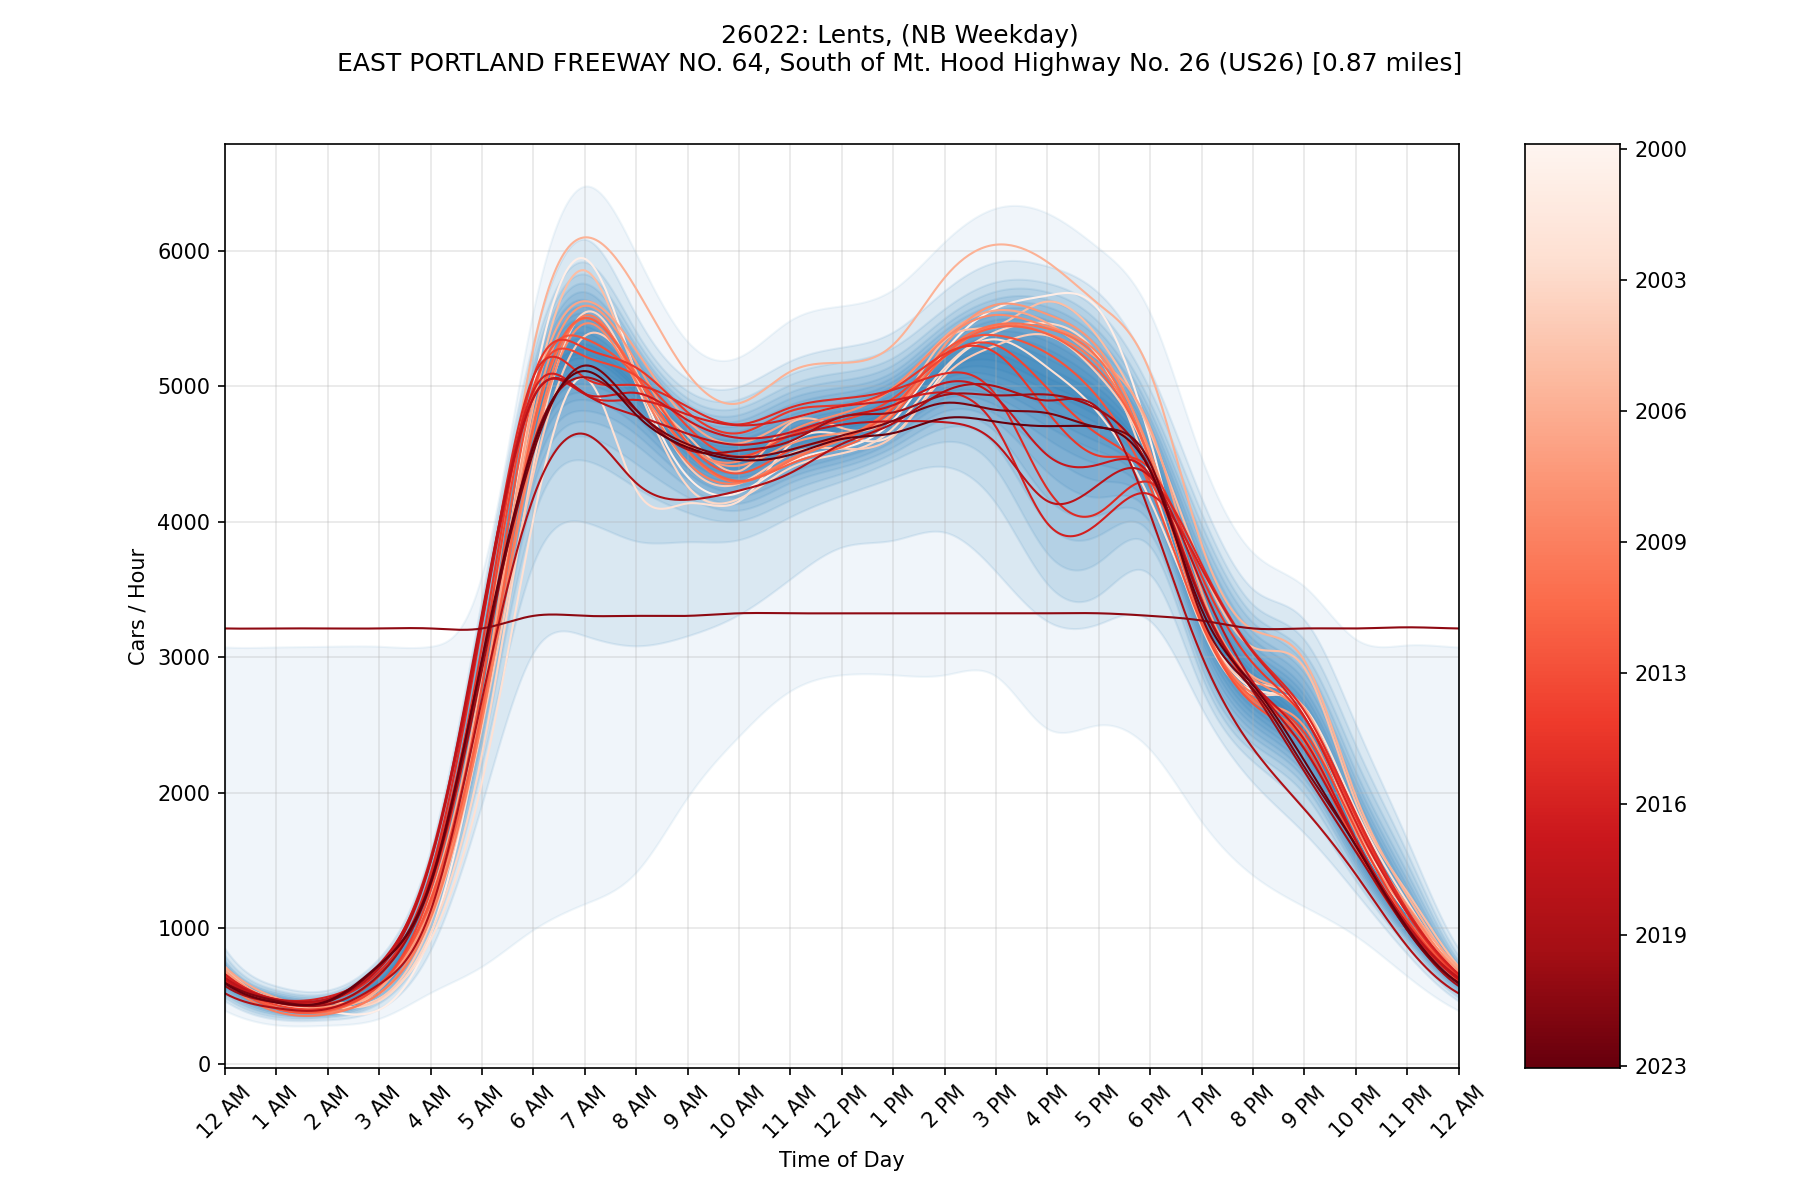
\includegraphics[width=\textwidth]{26022_Lents_NB_Weekday.png}
	\end{subfigure}
	\hfill
	\begin{subfigure}{0.45\textwidth}
		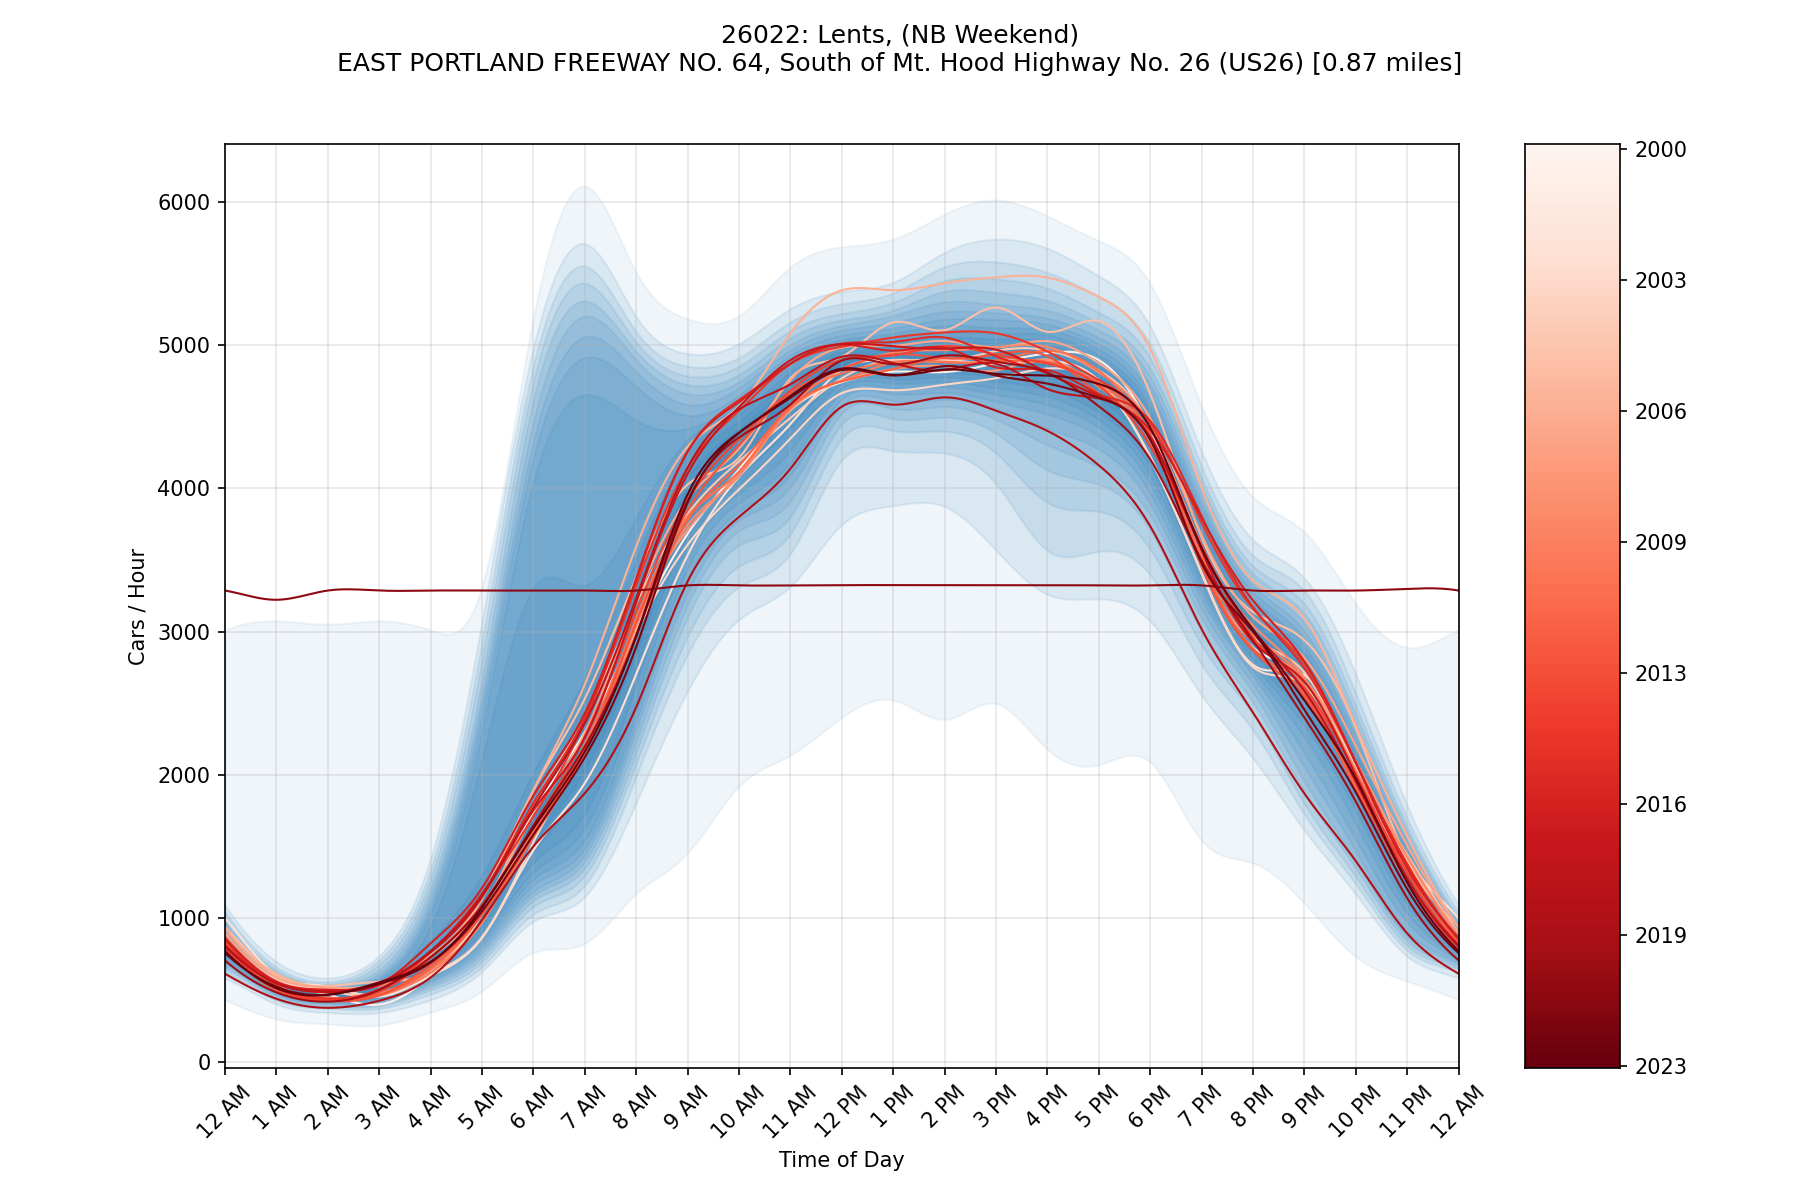
\includegraphics[width=\textwidth]{26022_Lents_NB_Weekend.png}
	\end{subfigure}

	\begin{subfigure}{0.45\textwidth}
		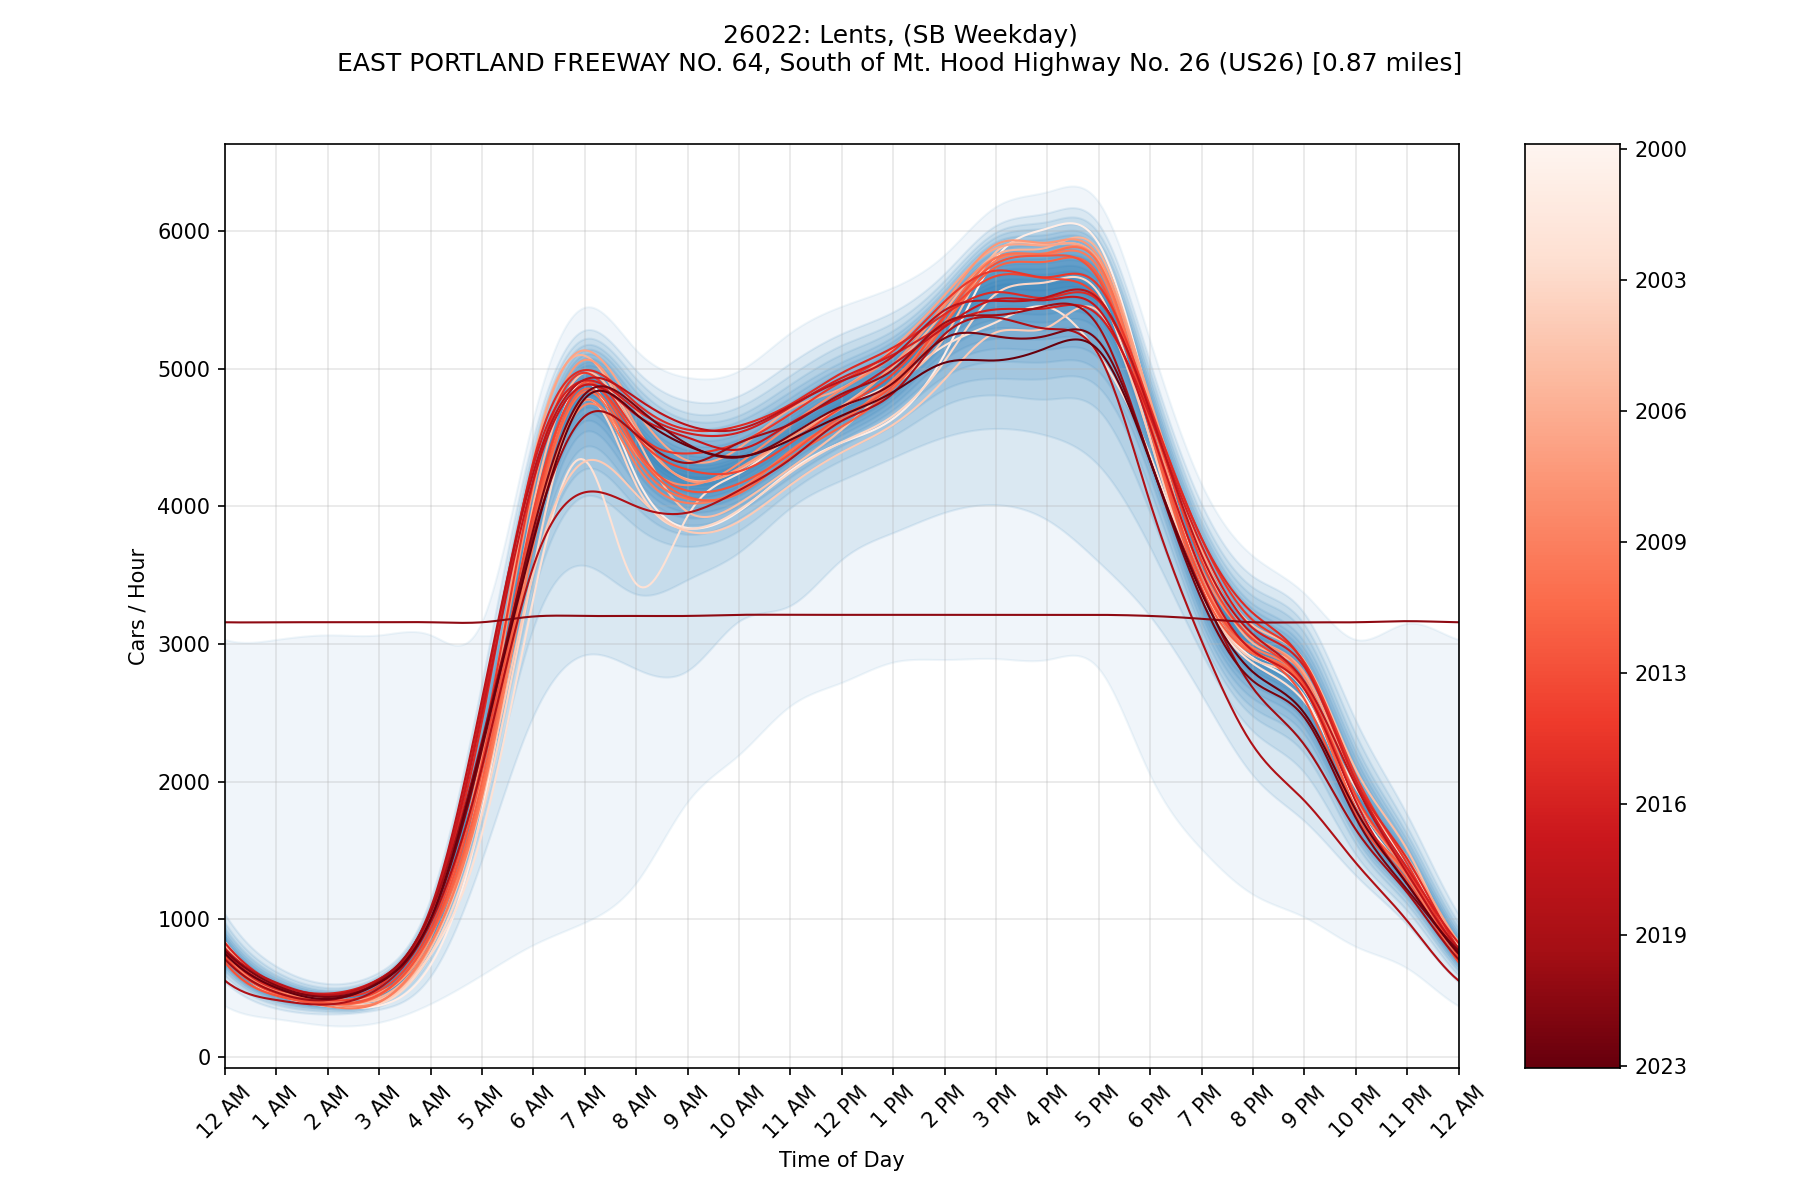
\includegraphics[width=\textwidth]{26022_Lents_SB_Weekday.png}
	\end{subfigure}
	\hfill
	\begin{subfigure}{0.45\textwidth}
		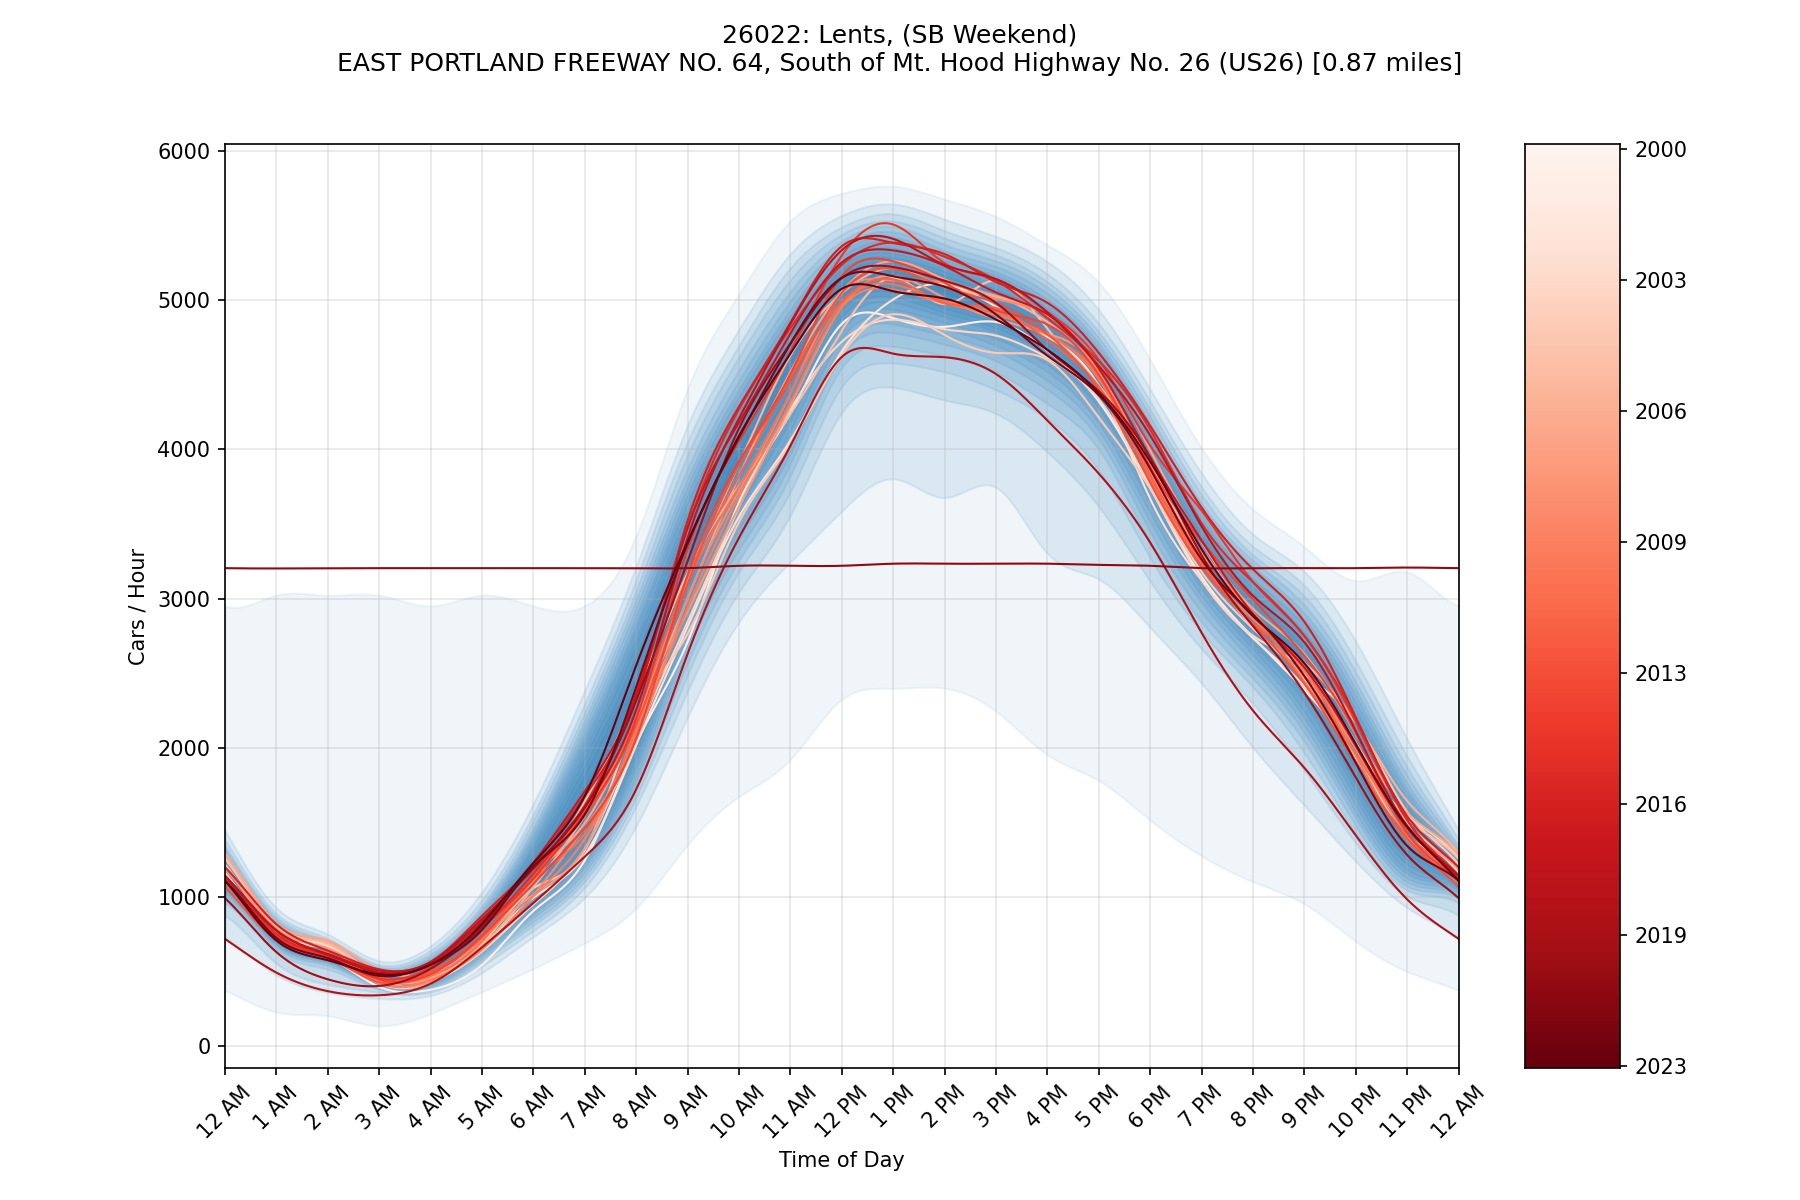
\includegraphics[width=\textwidth]{26022_Lents_SB_Weekend.png}
	\end{subfigure}
\end{figure}

\begin{figure}[htbp]
	\centering
	\begin{subfigure}{0.45\textwidth}
		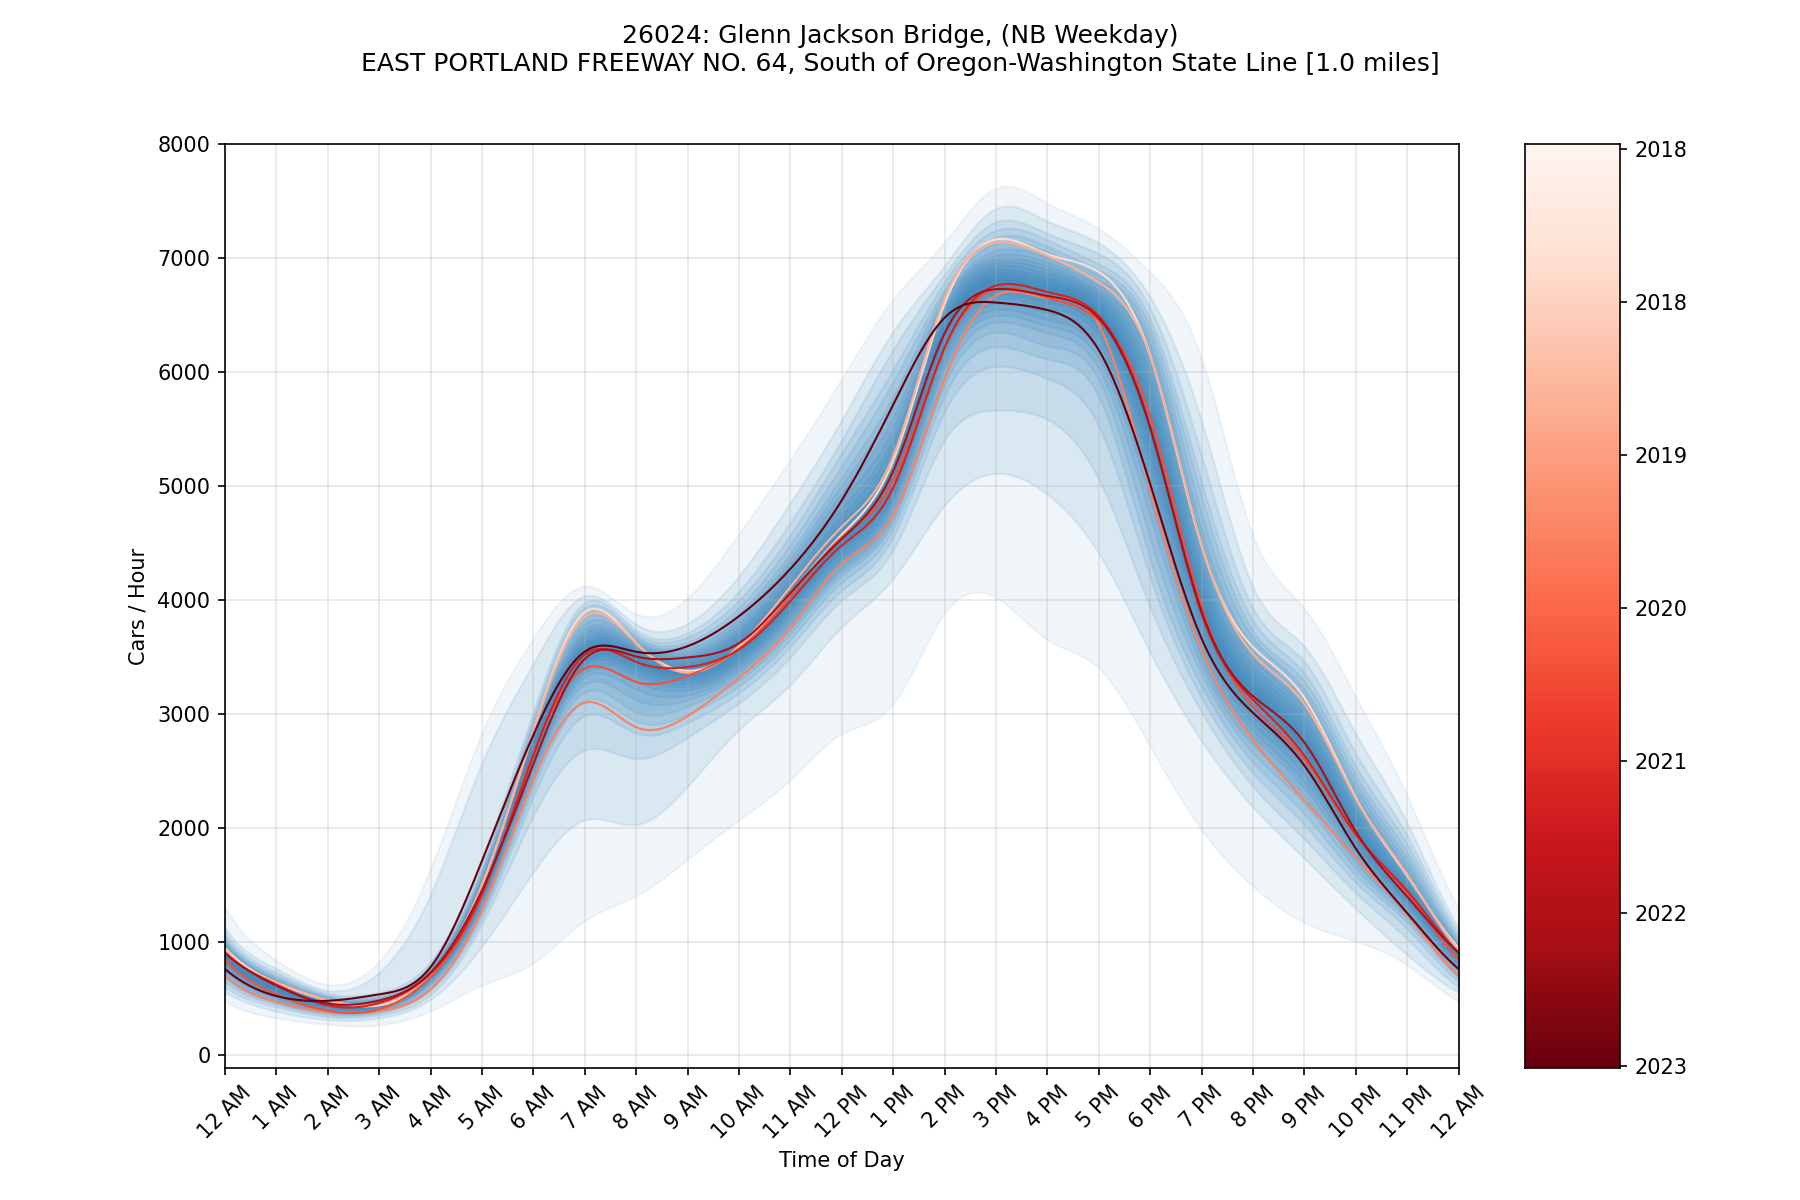
\includegraphics[width=\textwidth]{26024_Glenn-Jackson-Bridge_NB_Weekday.png}
	\end{subfigure}
	\hfill
	\begin{subfigure}{0.45\textwidth}
		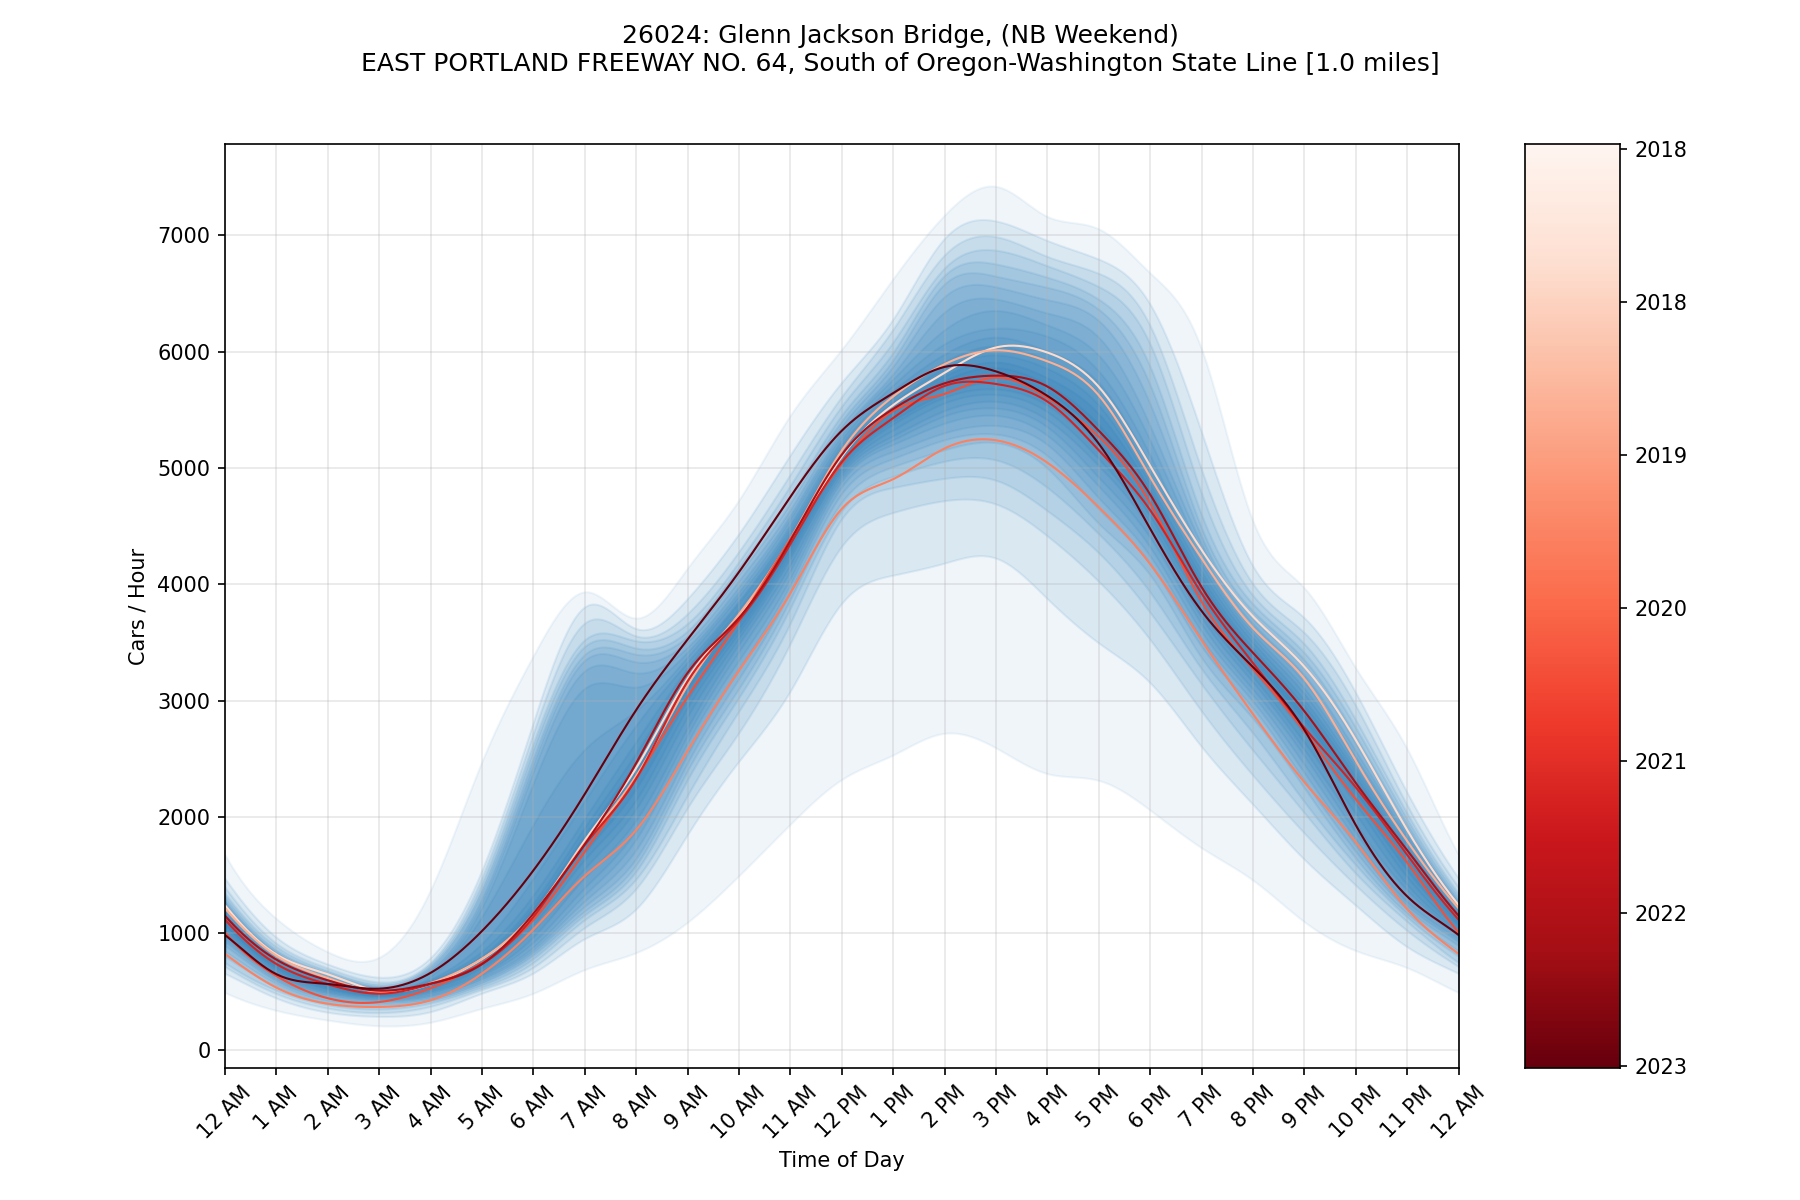
\includegraphics[width=\textwidth]{26024_Glenn-Jackson-Bridge_NB_Weekend.png}
	\end{subfigure}

	\begin{subfigure}{0.45\textwidth}
		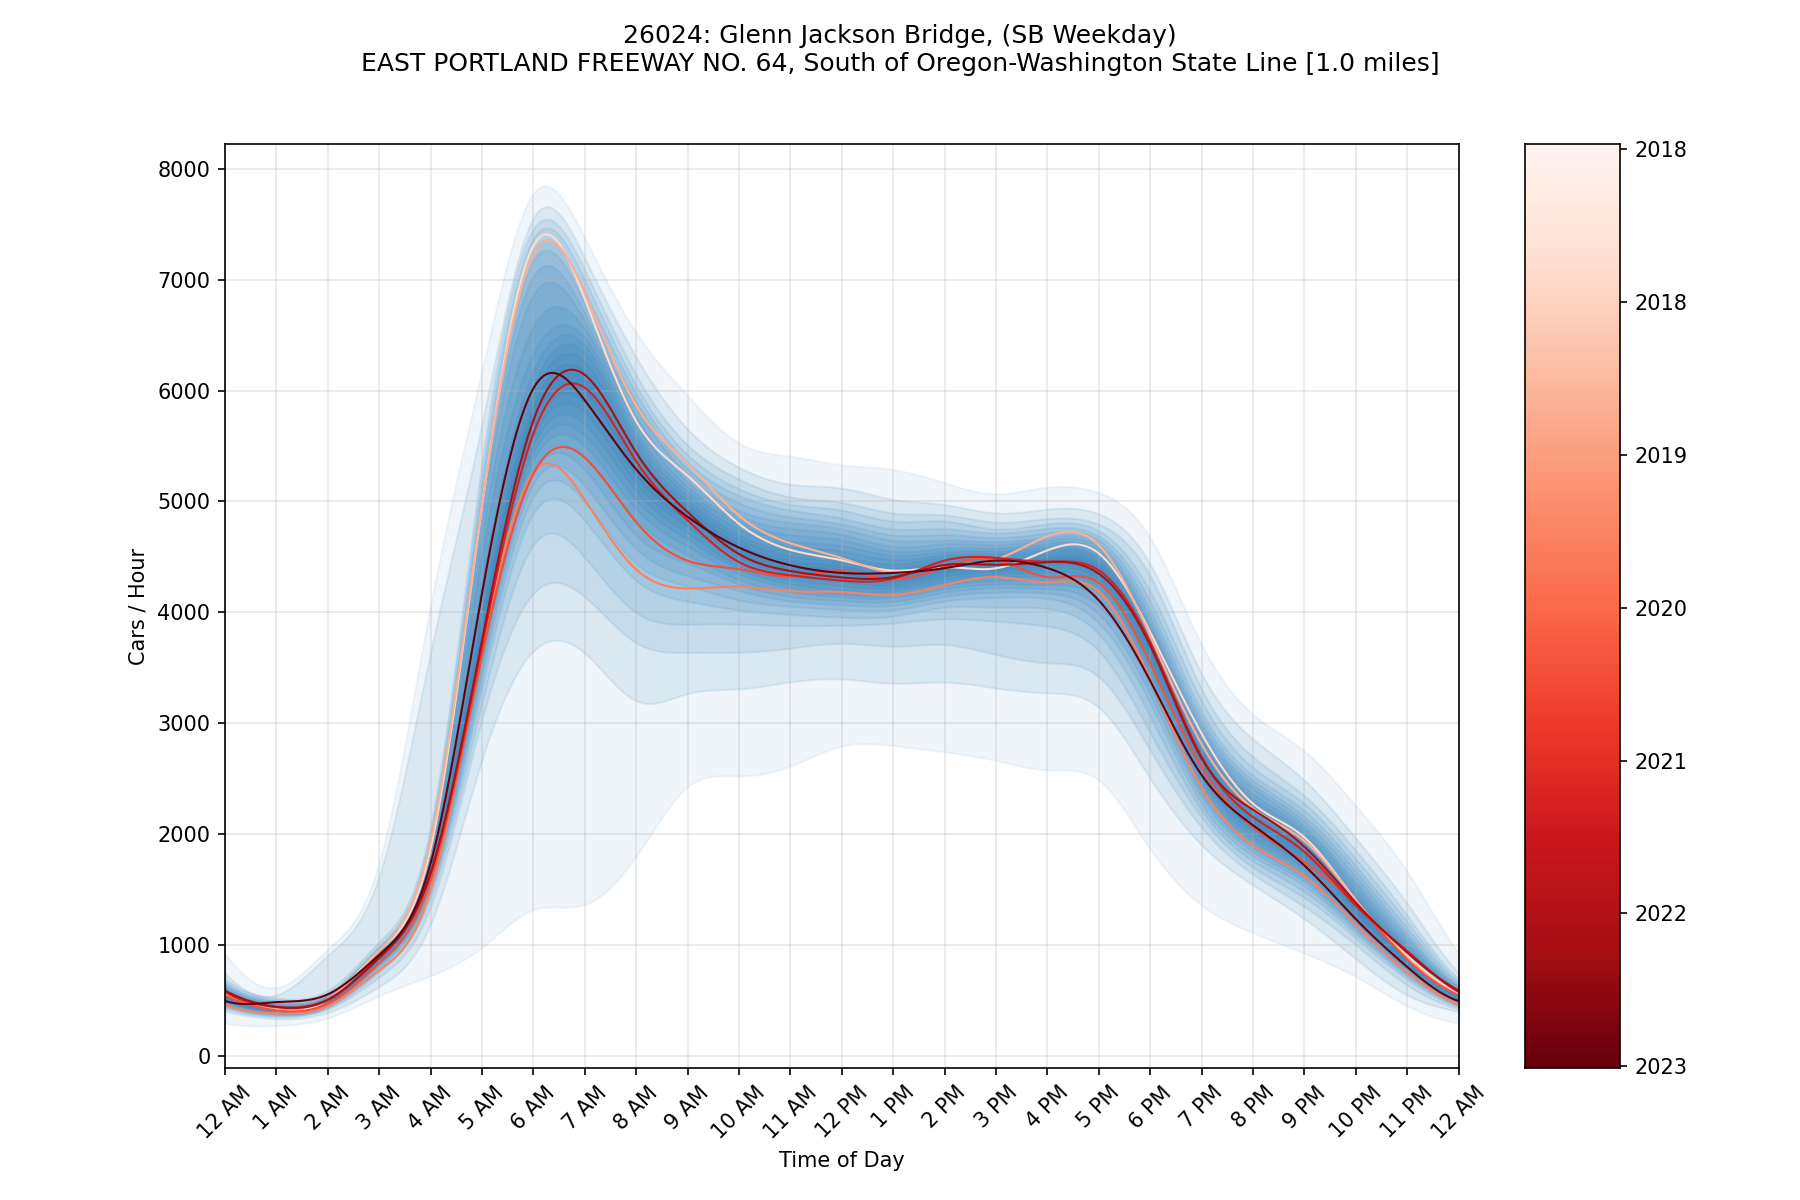
\includegraphics[width=\textwidth]{26024_Glenn-Jackson-Bridge_SB_Weekday.png}
	\end{subfigure}
	\hfill
	\begin{subfigure}{0.45\textwidth}
		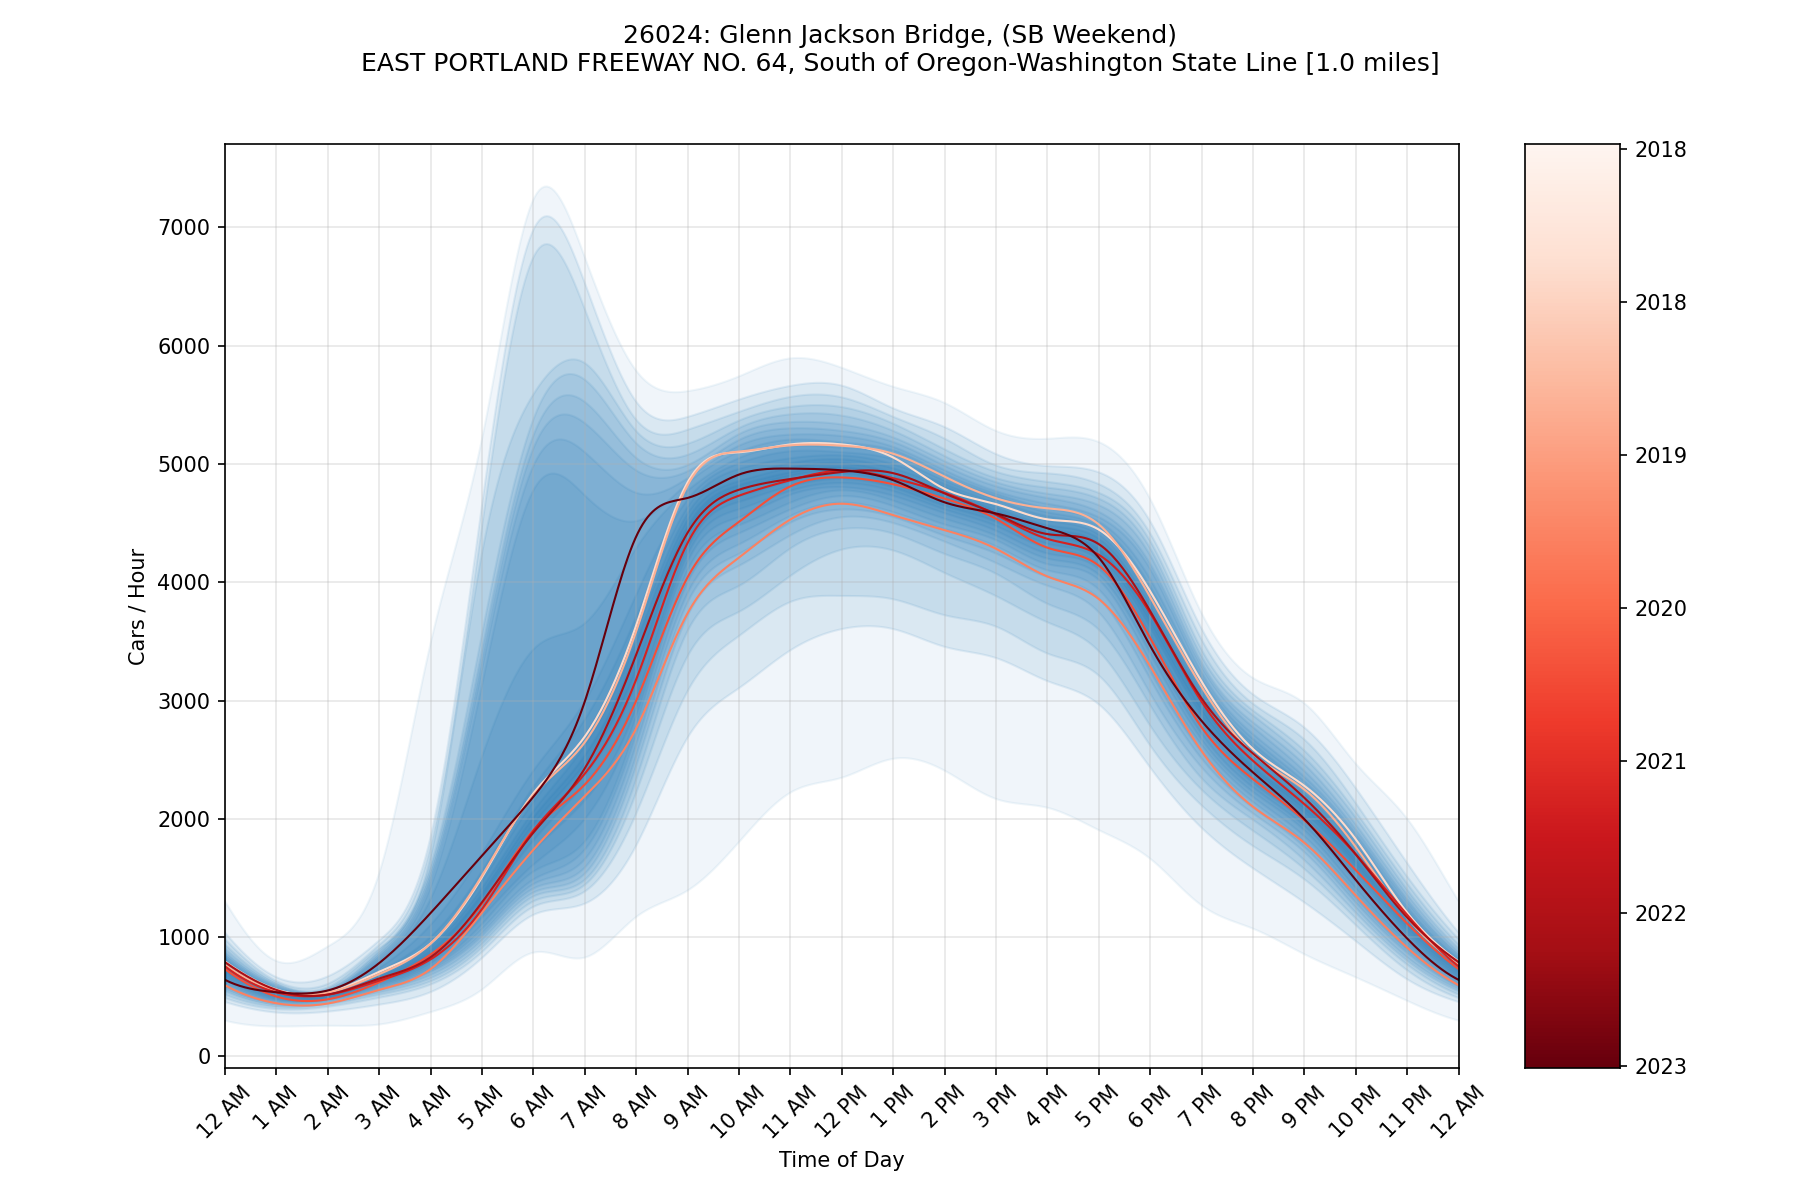
\includegraphics[width=\textwidth]{26024_Glenn-Jackson-Bridge_SB_Weekend.png}
	\end{subfigure}
\end{figure}

\begin{figure}[htbp]
	\centering
	\begin{subfigure}{0.45\textwidth}
		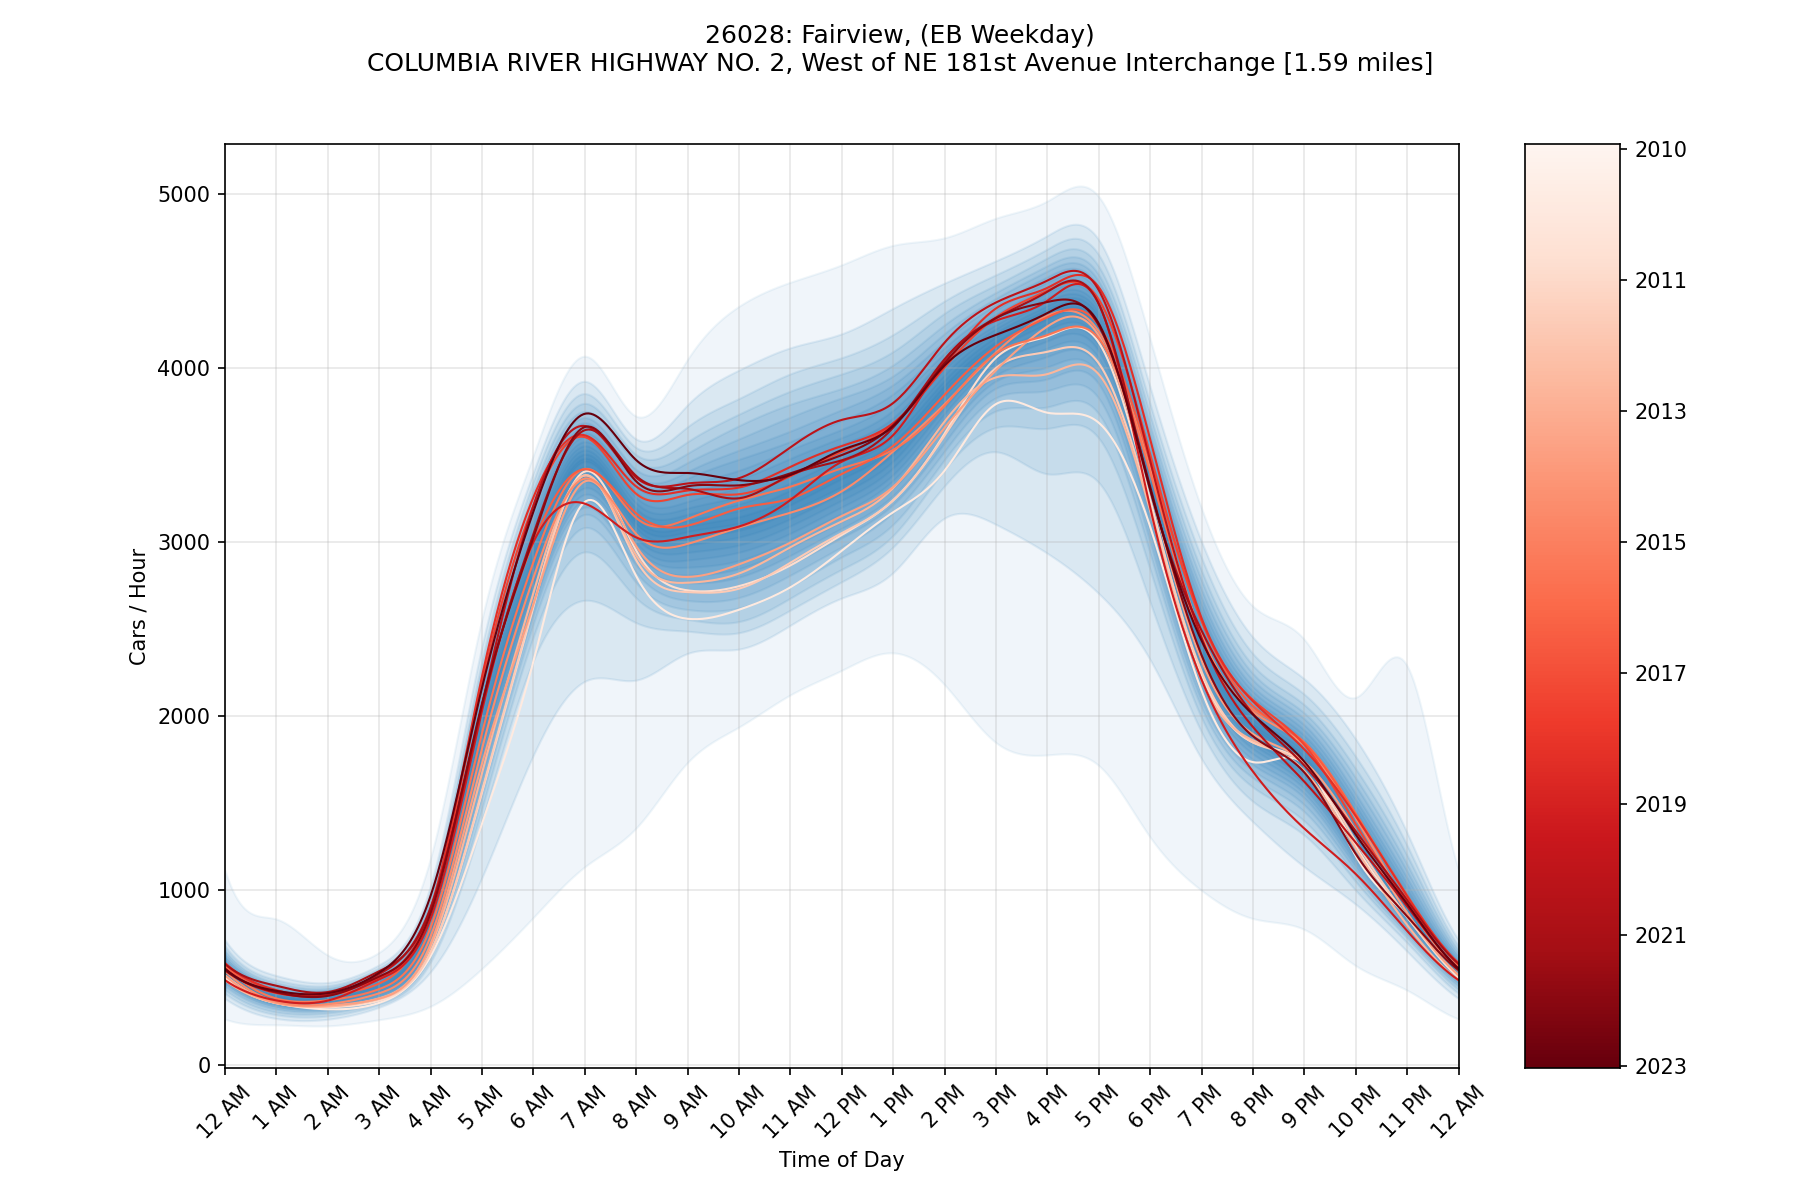
\includegraphics[width=\textwidth]{26028_Fairview_EB_Weekday.png}
	\end{subfigure}
	\hfill
	\begin{subfigure}{0.45\textwidth}
		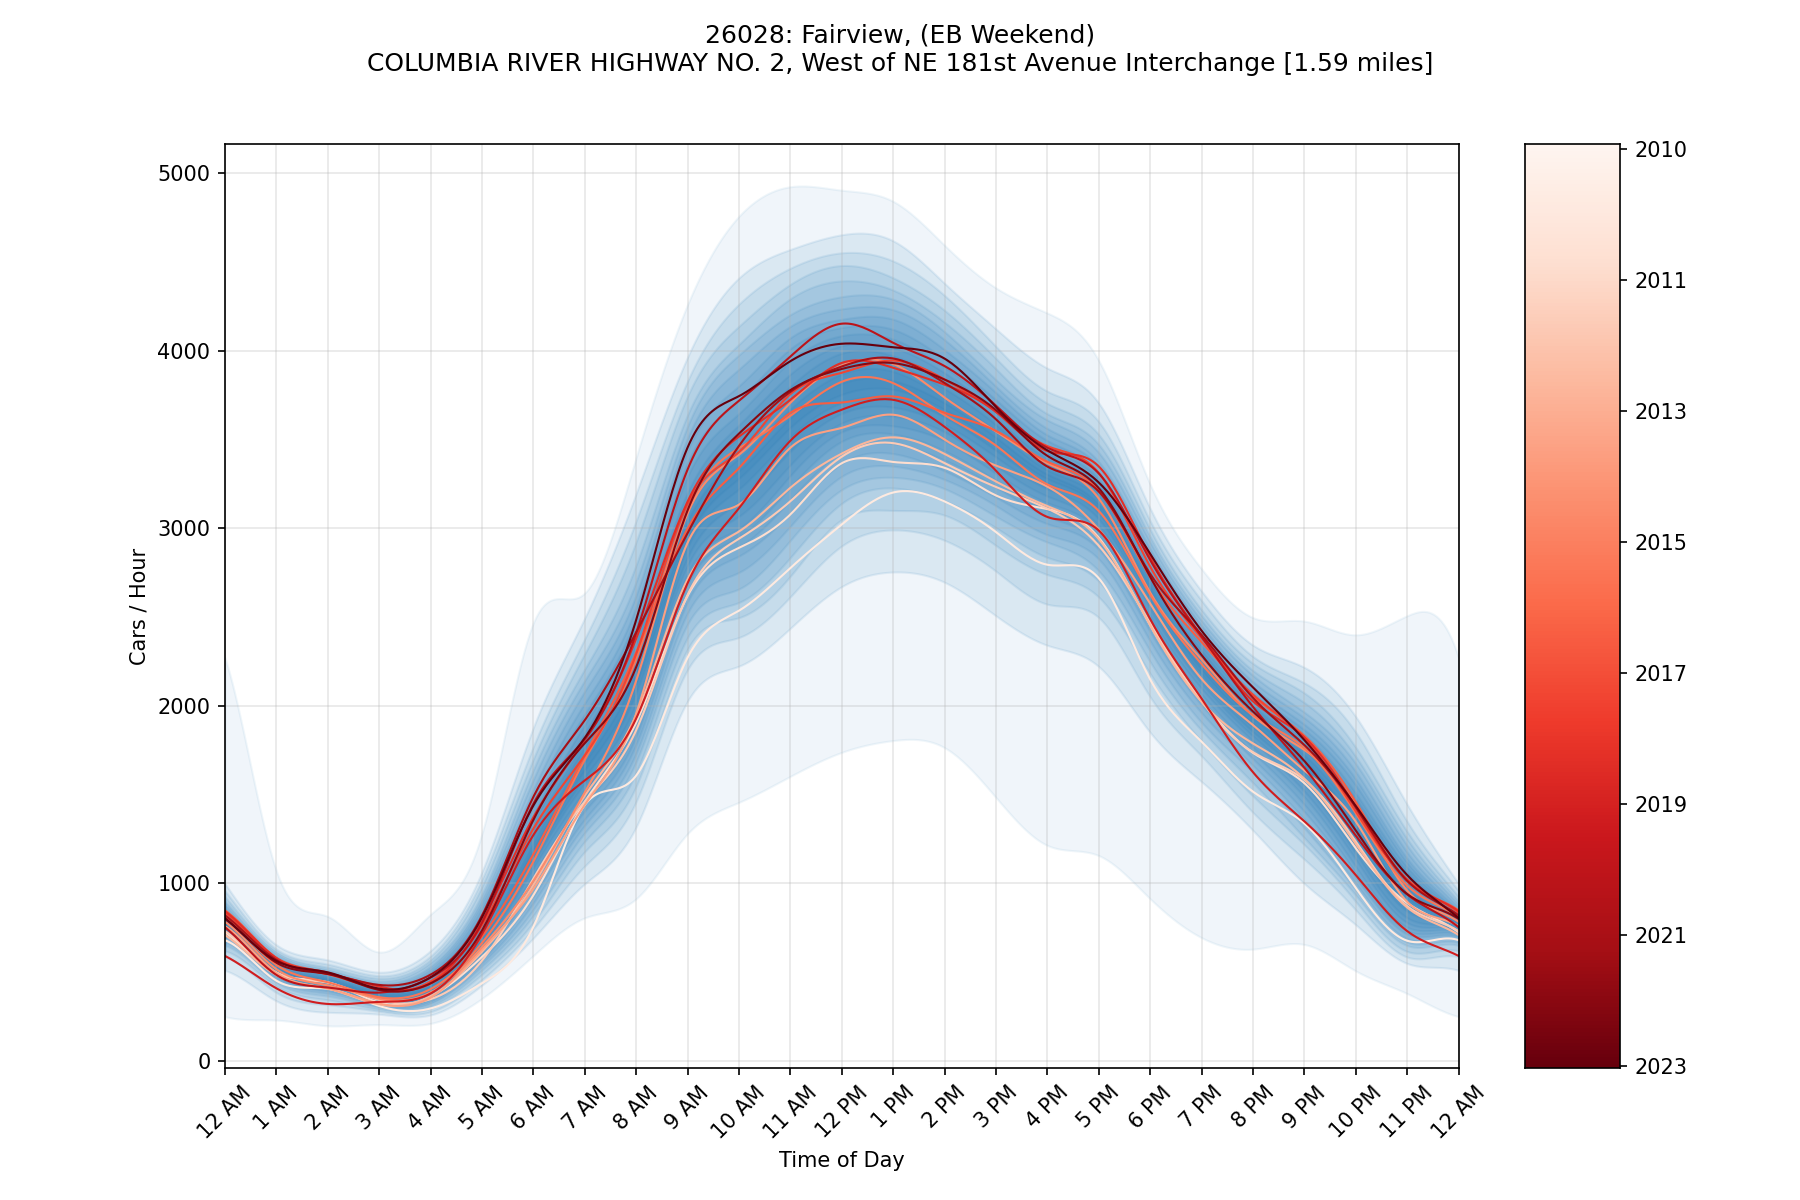
\includegraphics[width=\textwidth]{26028_Fairview_EB_Weekend.png}
	\end{subfigure}

	\begin{subfigure}{0.45\textwidth}
		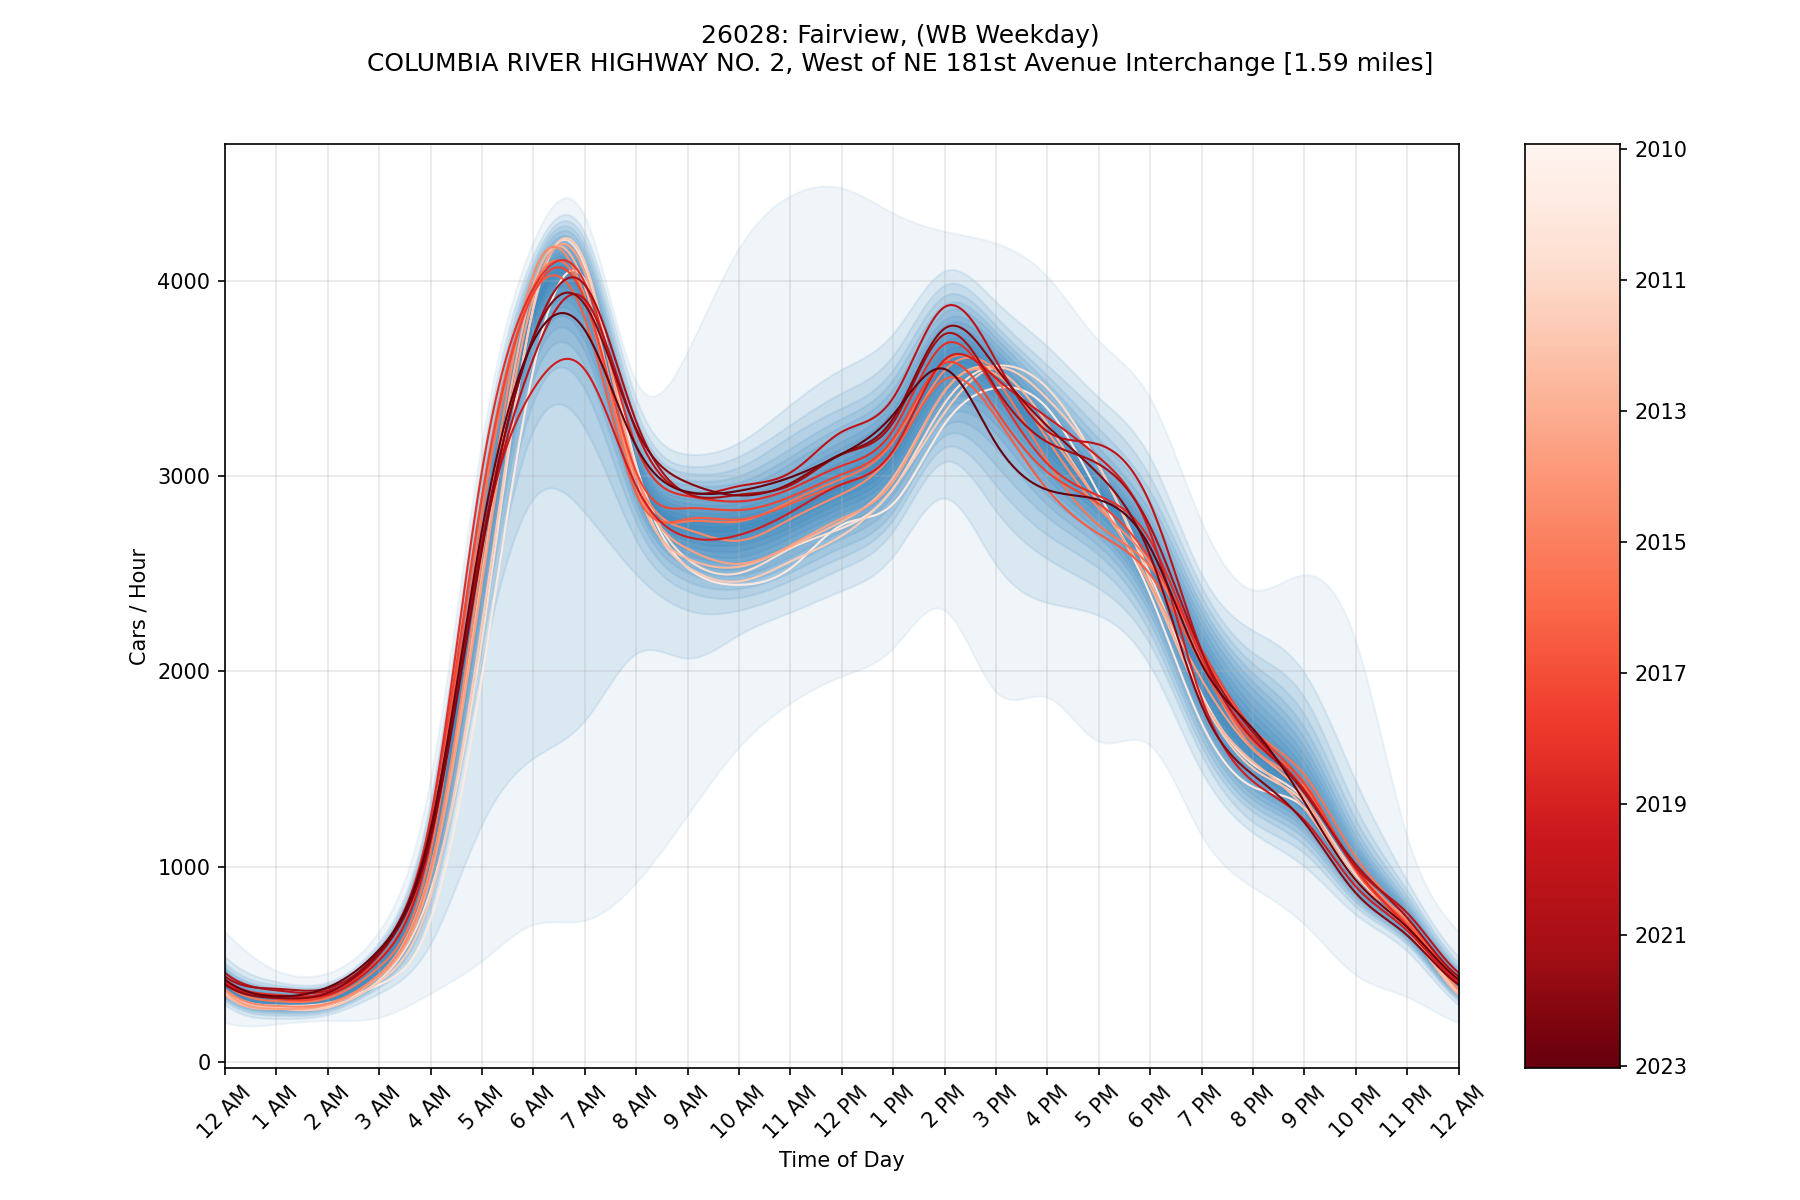
\includegraphics[width=\textwidth]{26028_Fairview_WB_Weekday.png}
	\end{subfigure}
	\hfill
	\begin{subfigure}{0.45\textwidth}
		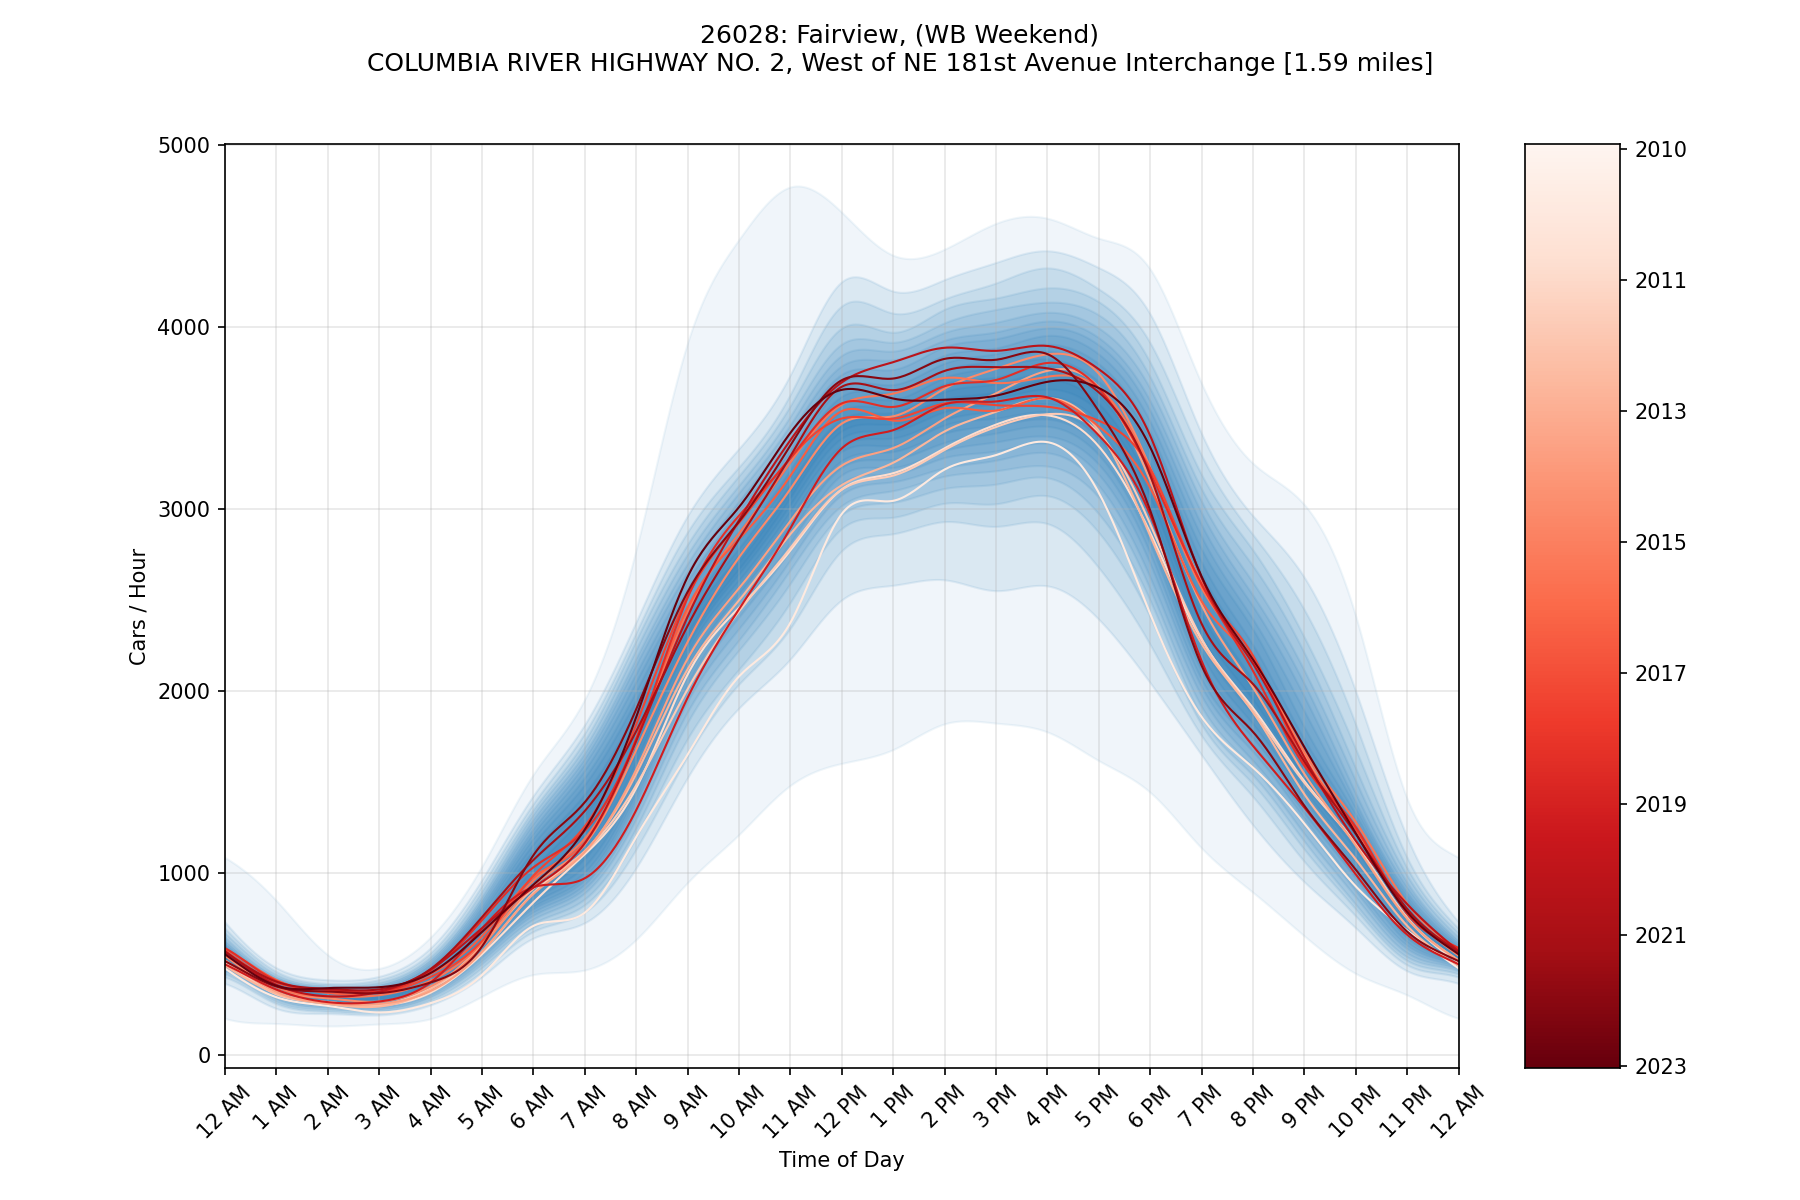
\includegraphics[width=\textwidth]{26028_Fairview_WB_Weekend.png}
	\end{subfigure}
\end{figure}

\begin{figure}[htbp]
	\centering
	\begin{subfigure}{0.45\textwidth}
		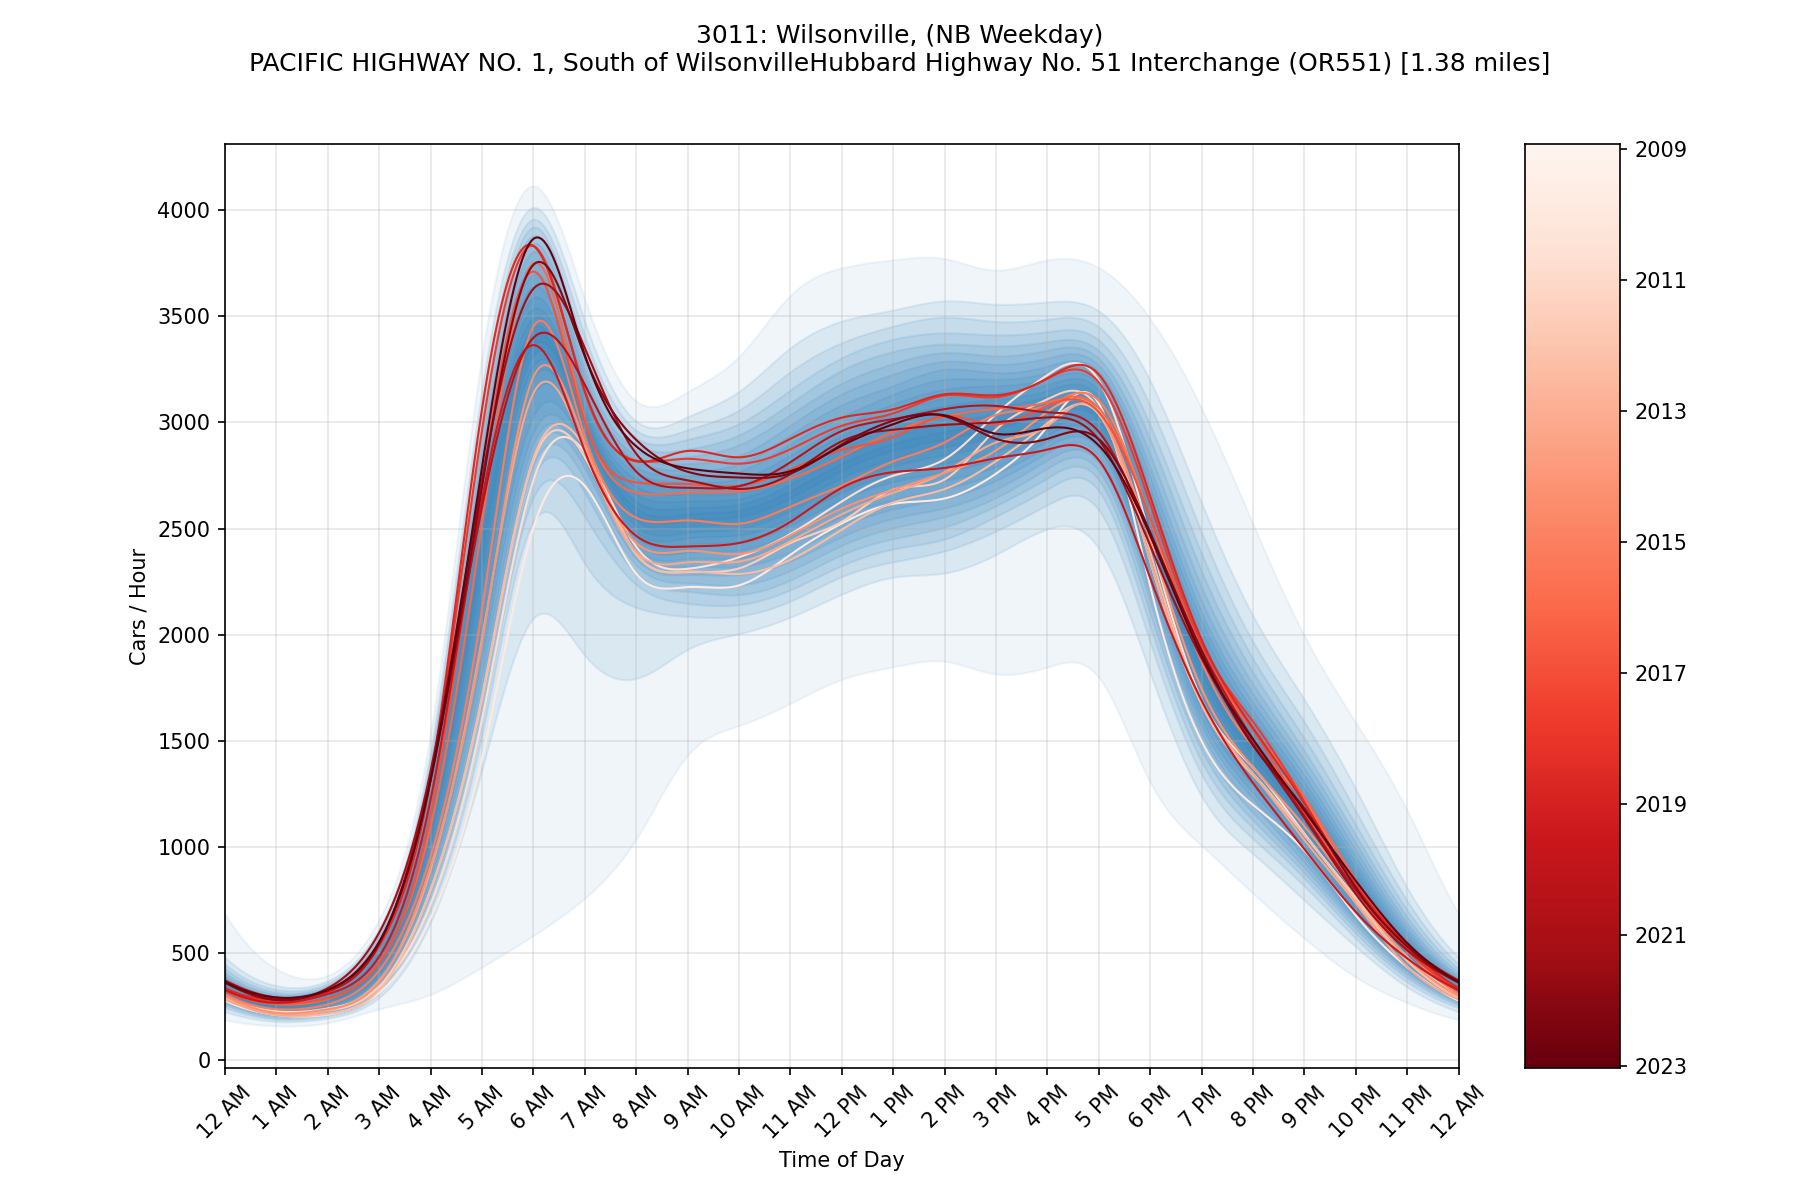
\includegraphics[width=\textwidth]{3011_Wilsonville_NB_Weekday.png}
	\end{subfigure}
	\hfill
	\begin{subfigure}{0.45\textwidth}
		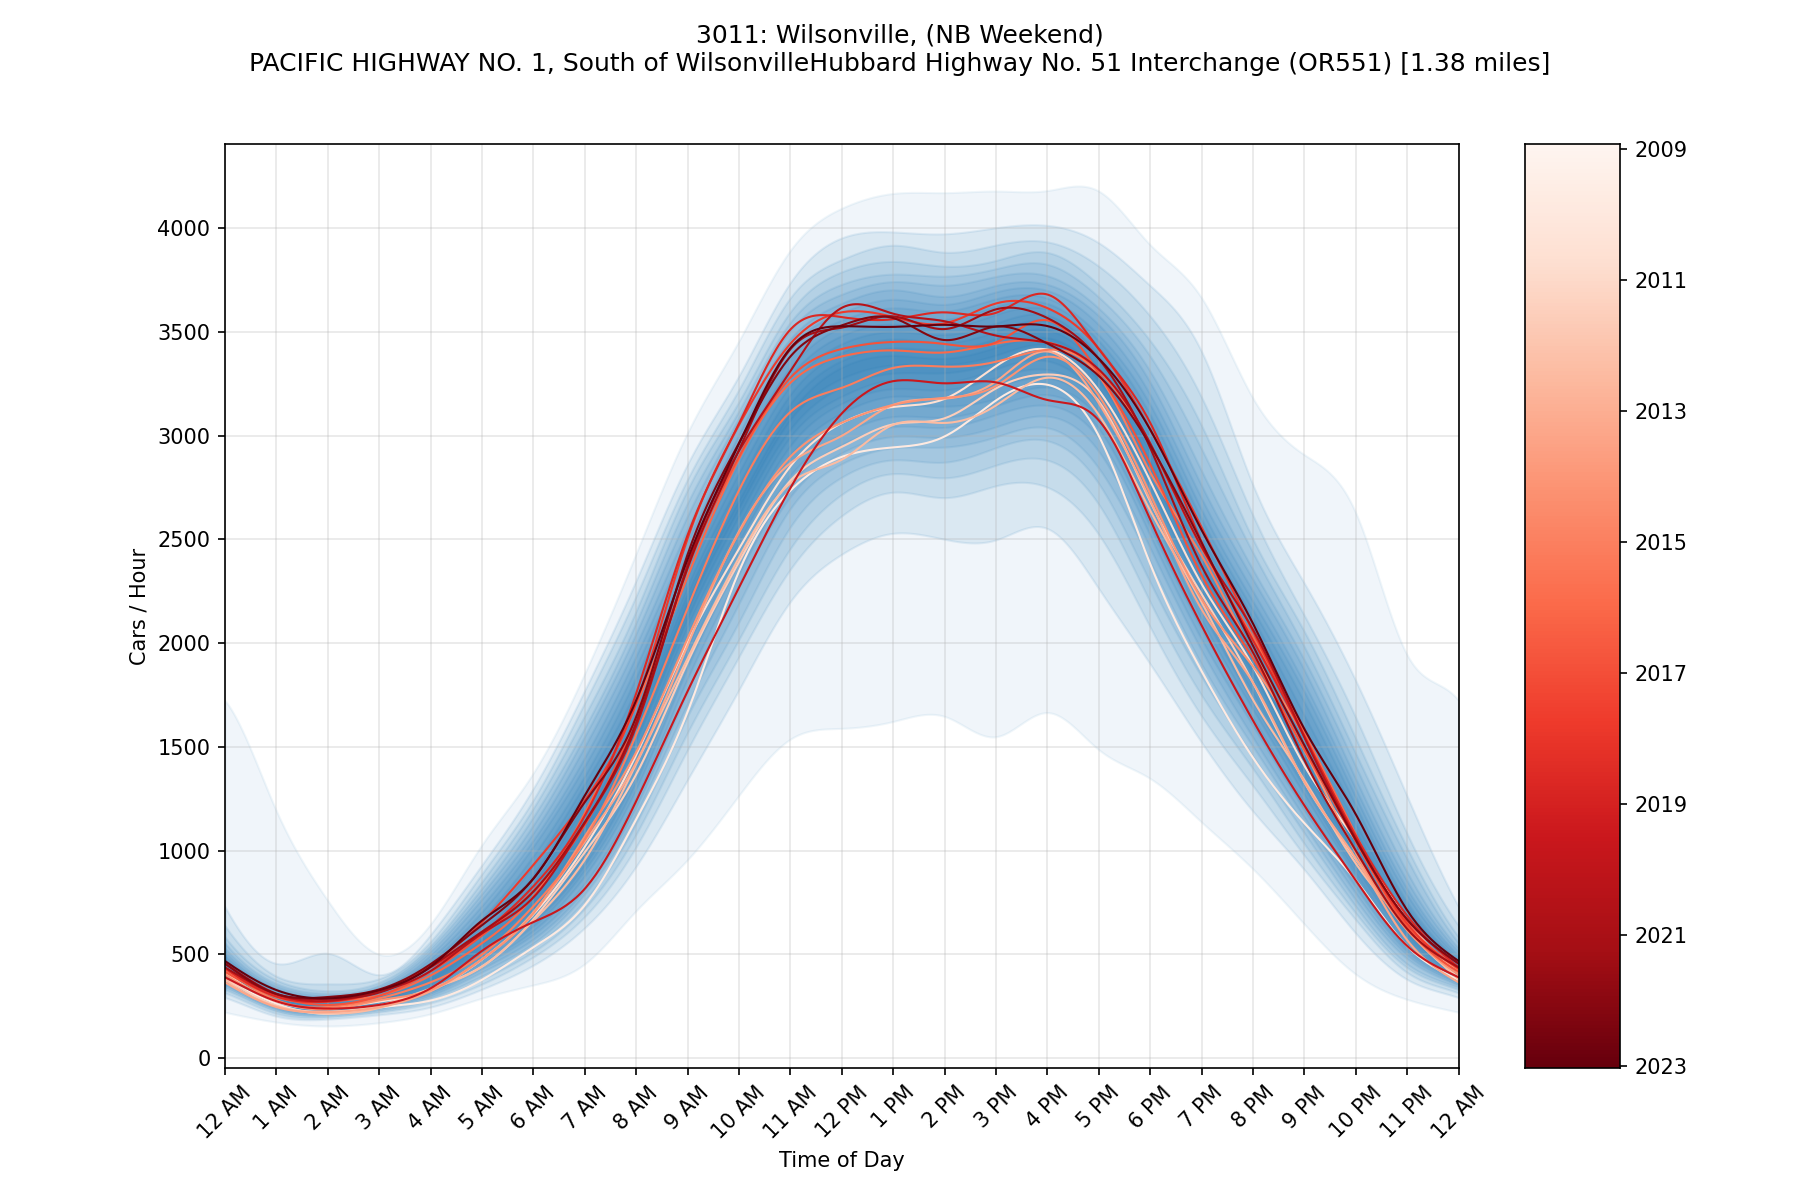
\includegraphics[width=\textwidth]{3011_Wilsonville_NB_Weekend.png}
	\end{subfigure}

	\begin{subfigure}{0.45\textwidth}
		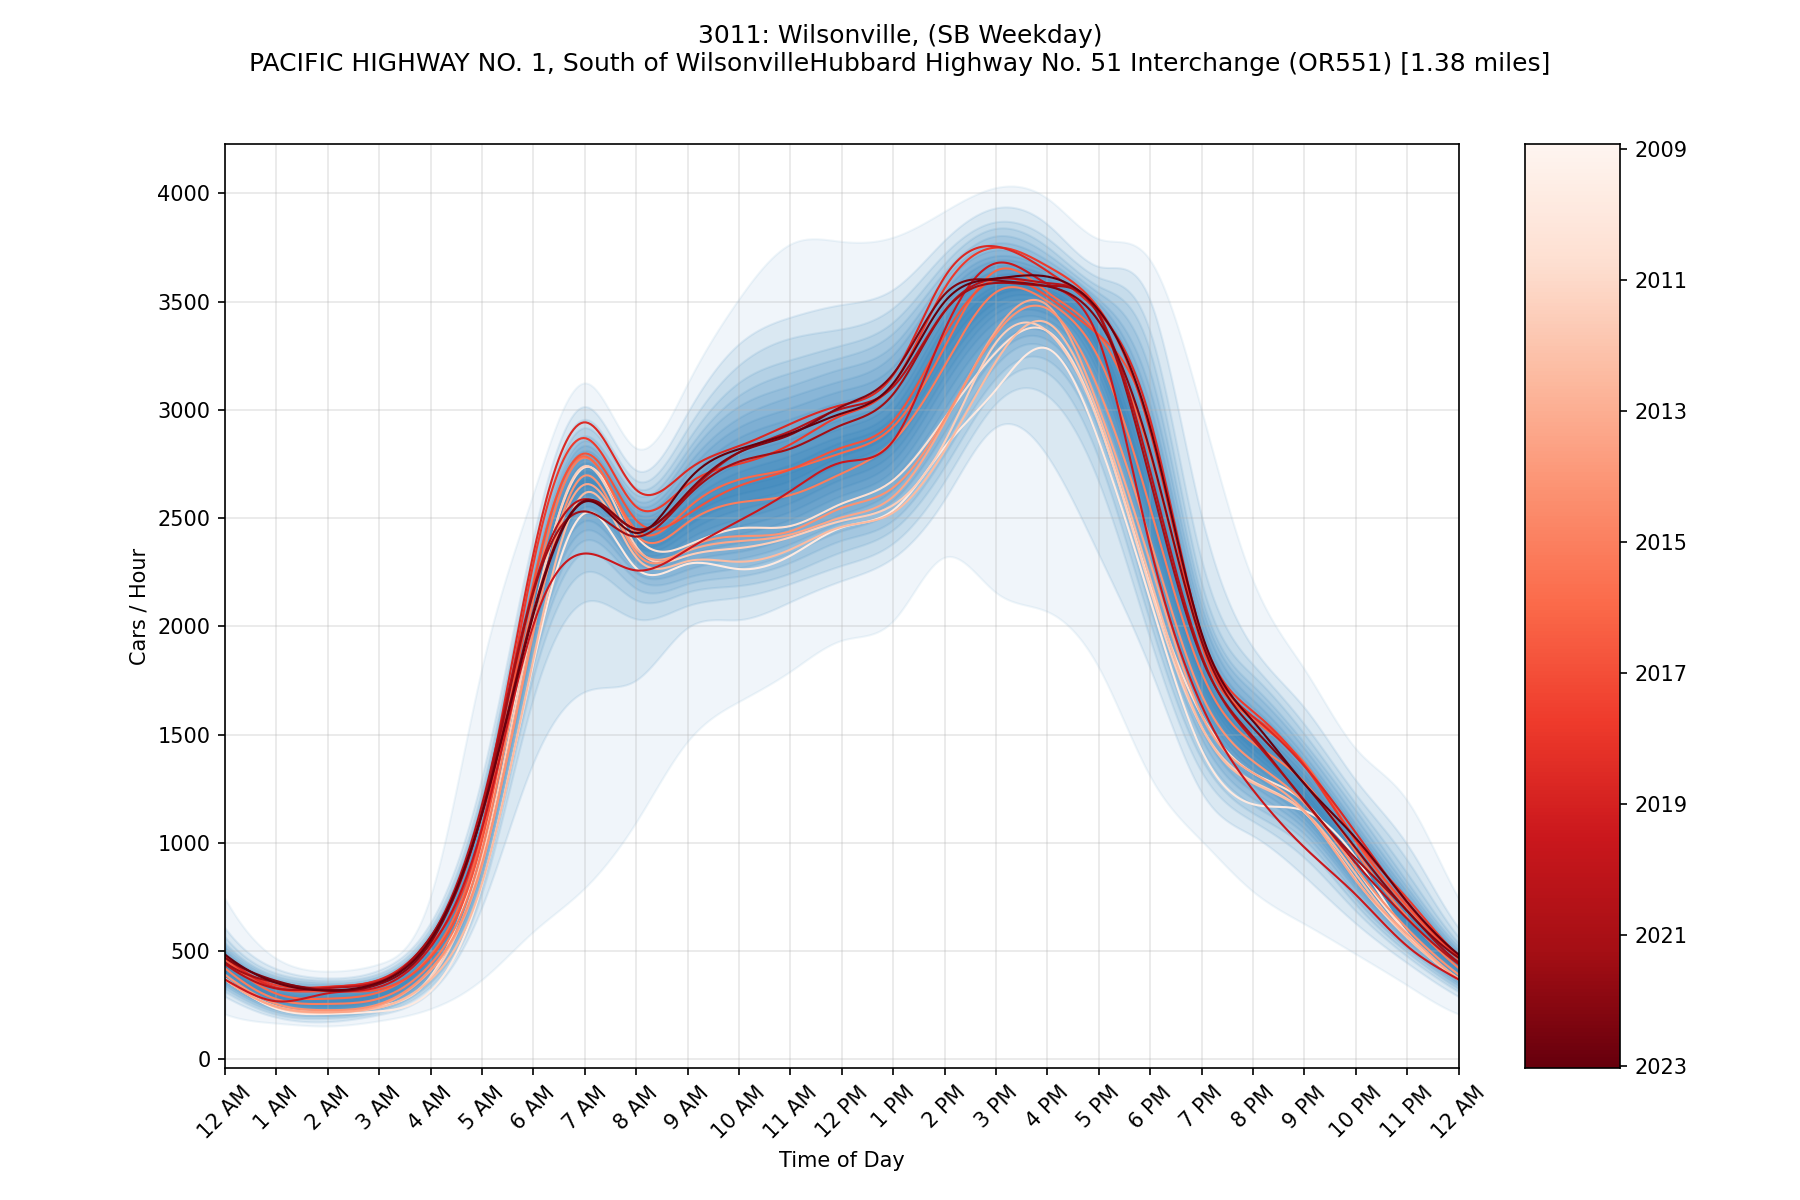
\includegraphics[width=\textwidth]{3011_Wilsonville_SB_Weekday.png}
	\end{subfigure}
	\hfill
	\begin{subfigure}{0.45\textwidth}
		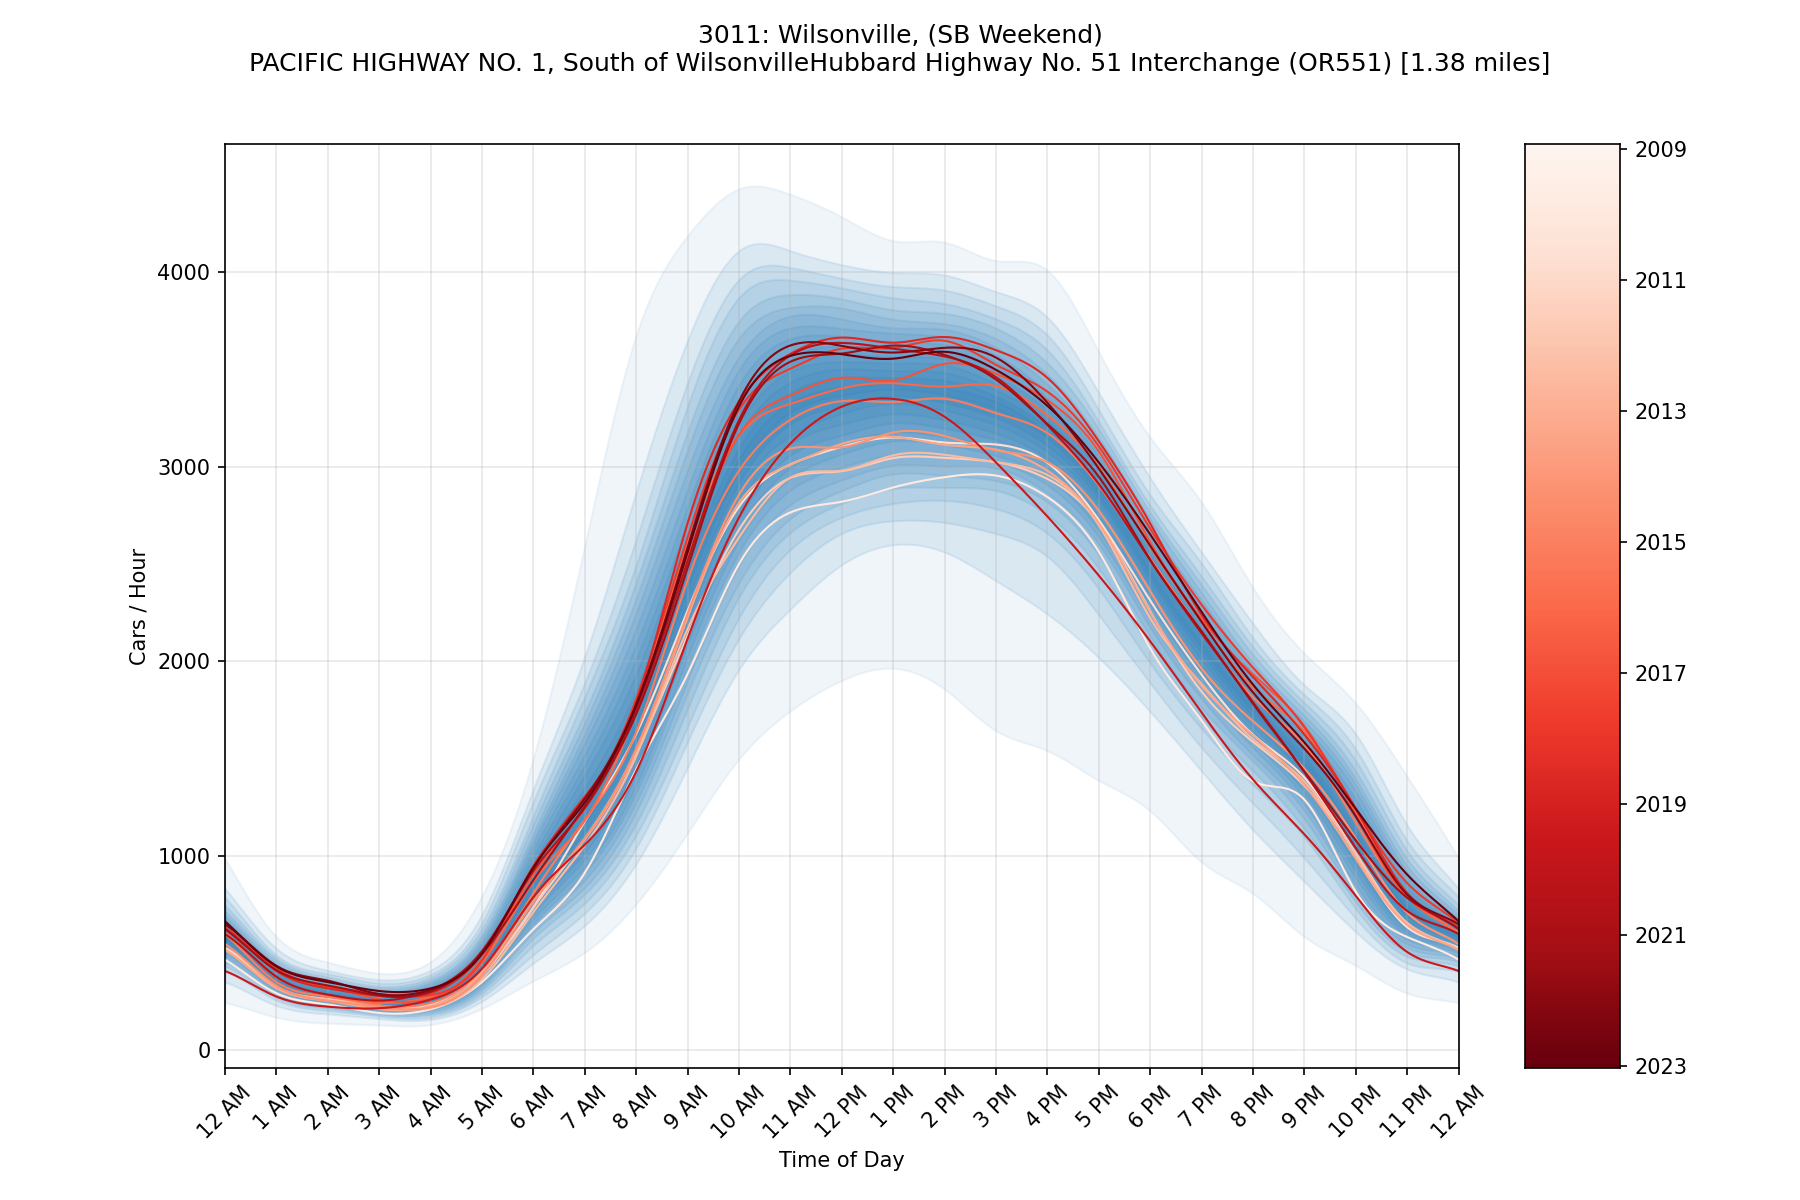
\includegraphics[width=\textwidth]{3011_Wilsonville_SB_Weekend.png}
	\end{subfigure}
\end{figure}

\begin{figure}[htbp]
	\centering
	\begin{subfigure}{0.45\textwidth}
		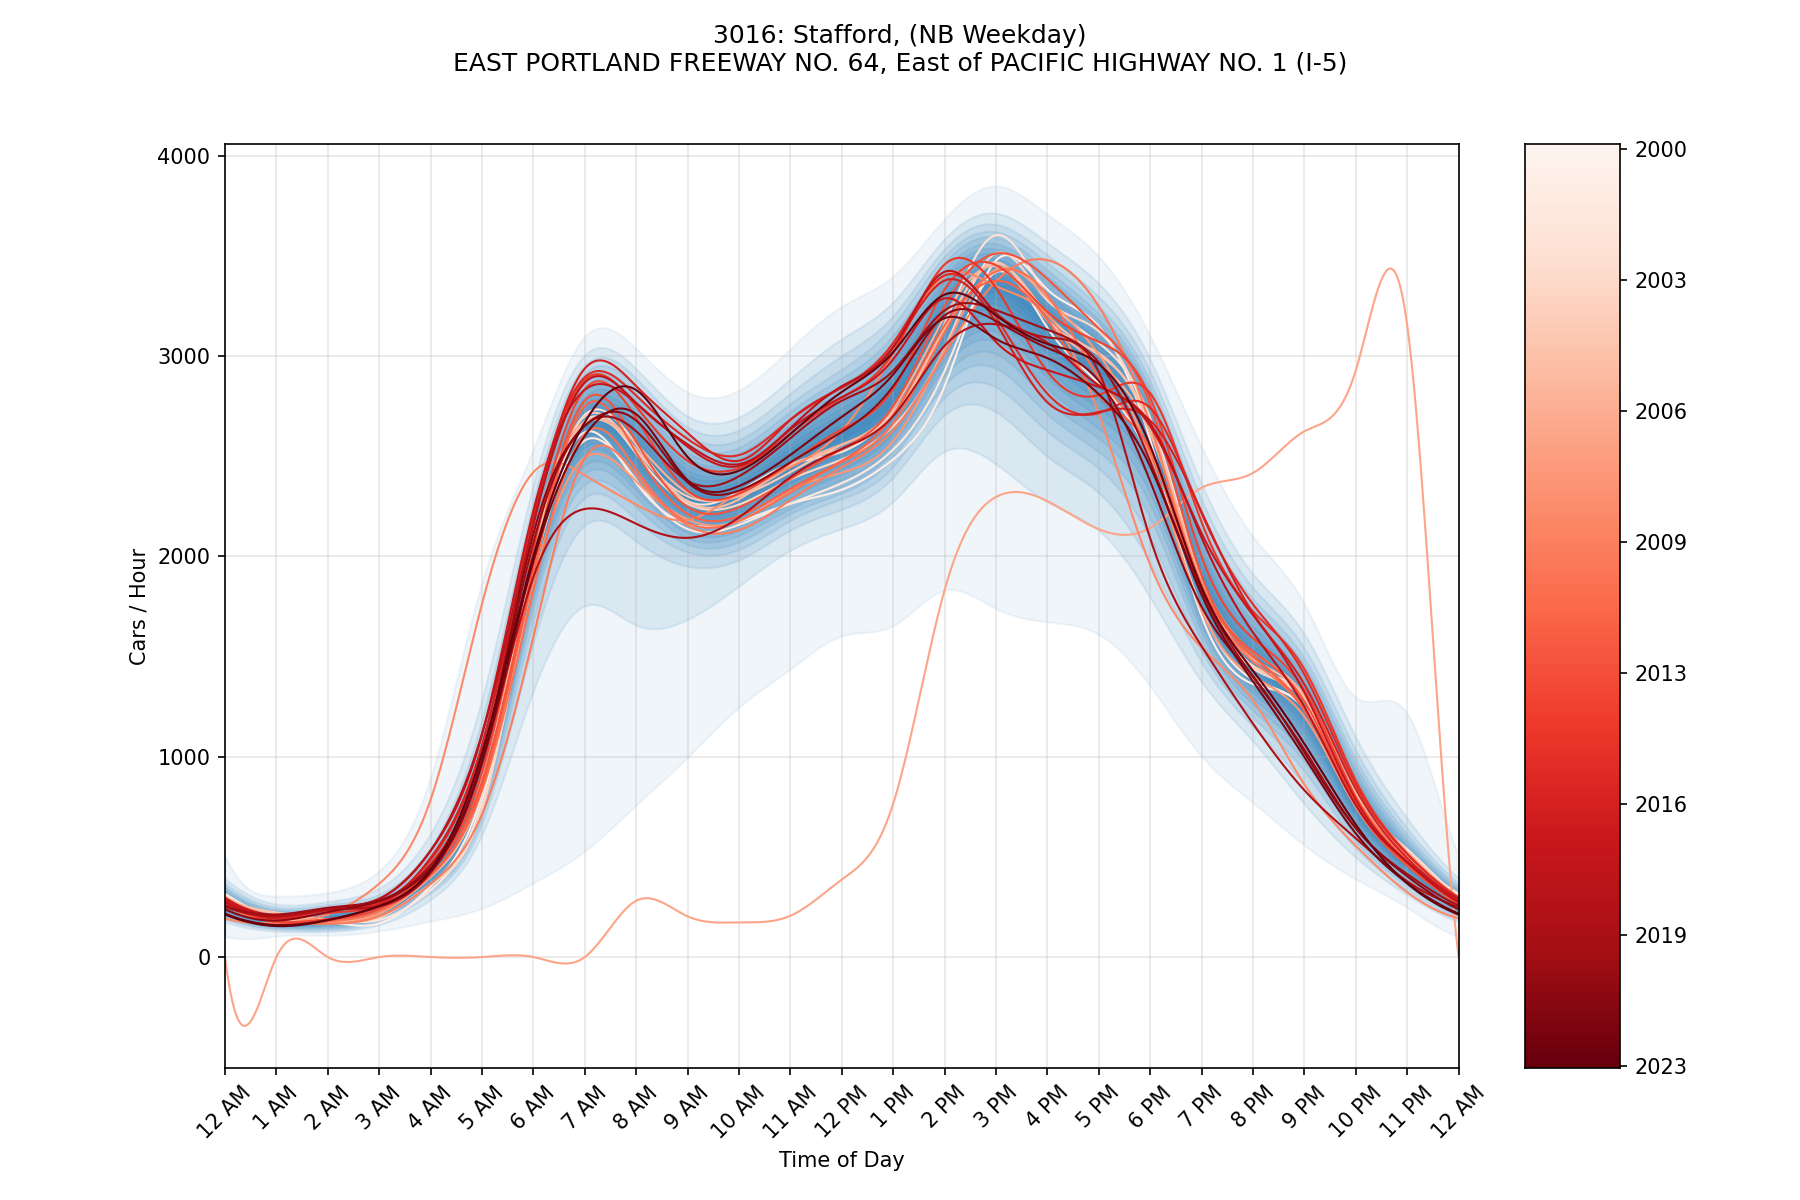
\includegraphics[width=\textwidth]{3016_Stafford_NB_Weekday.png}
	\end{subfigure}
	\hfill
	\begin{subfigure}{0.45\textwidth}
		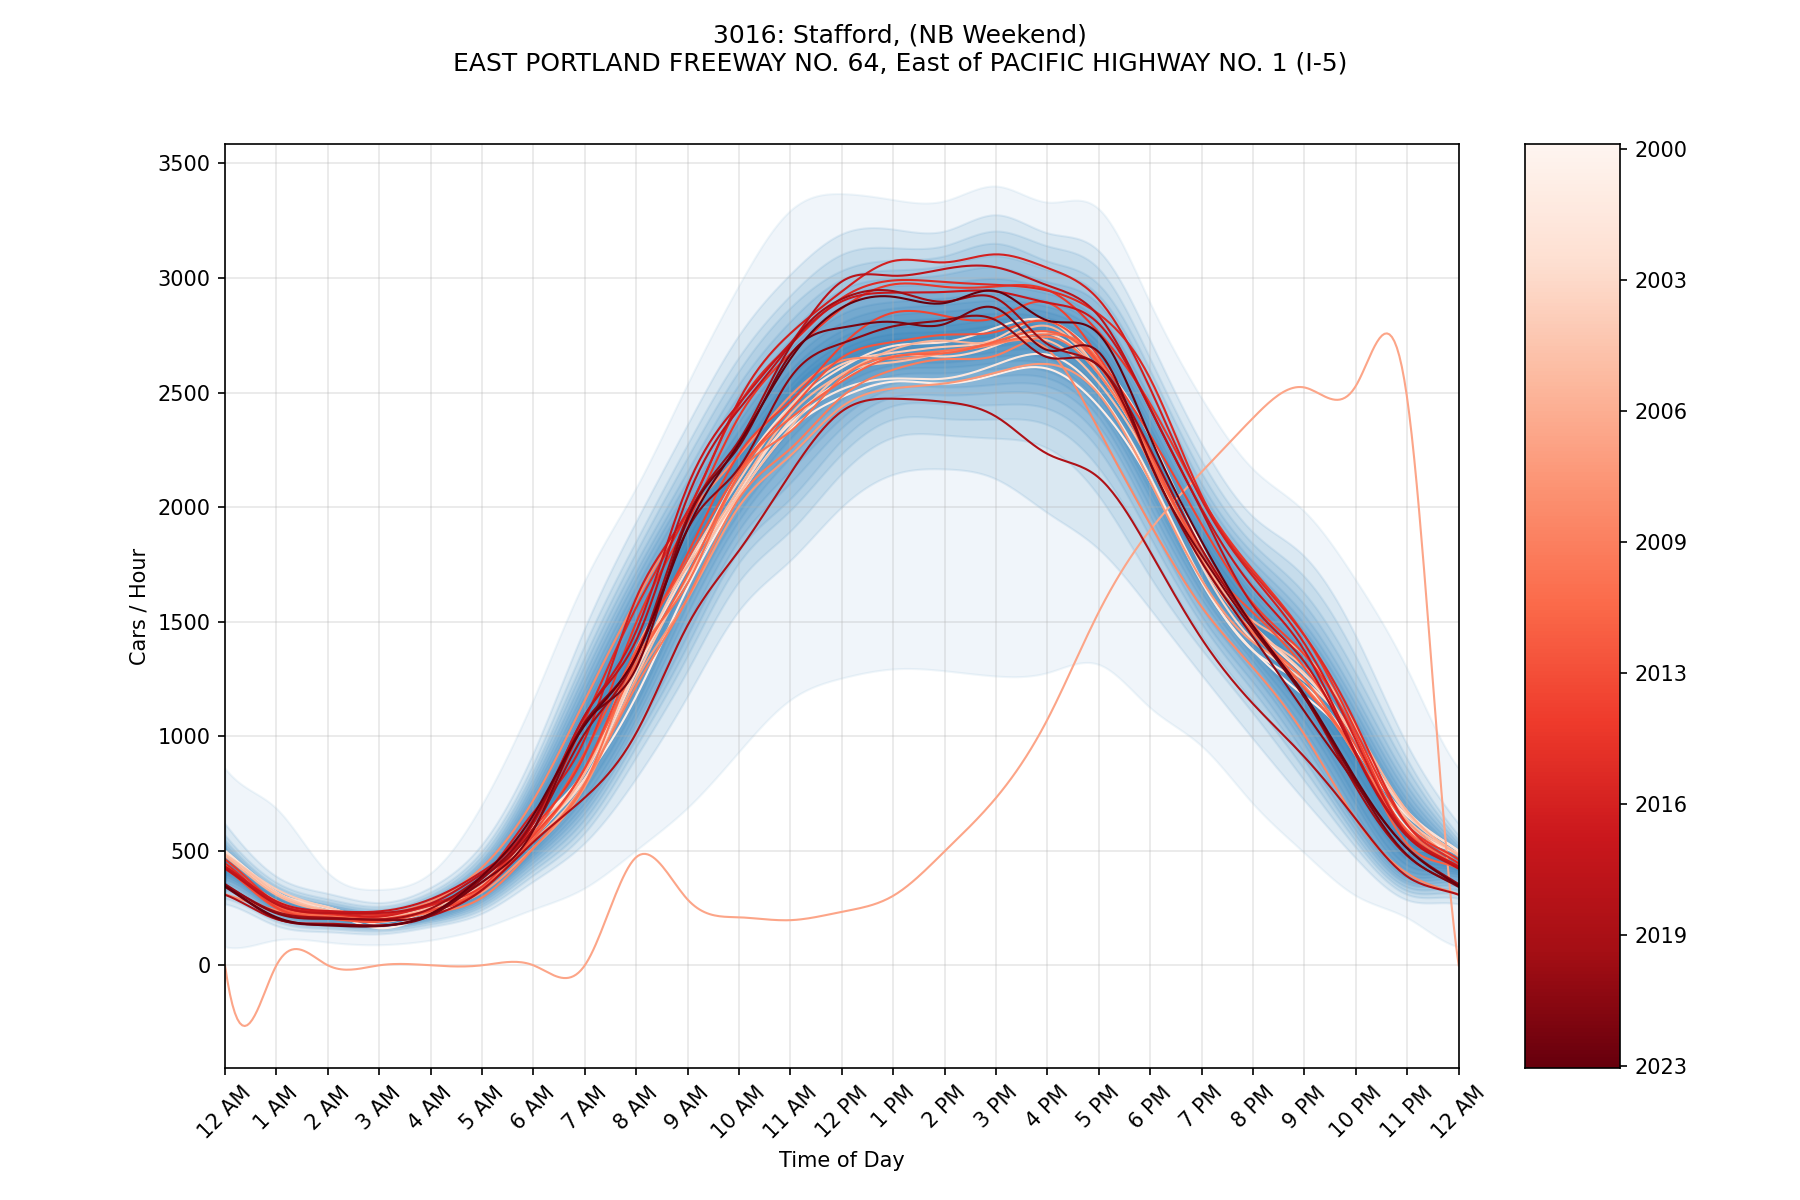
\includegraphics[width=\textwidth]{3016_Stafford_NB_Weekend.png}
	\end{subfigure}

	\begin{subfigure}{0.45\textwidth}
		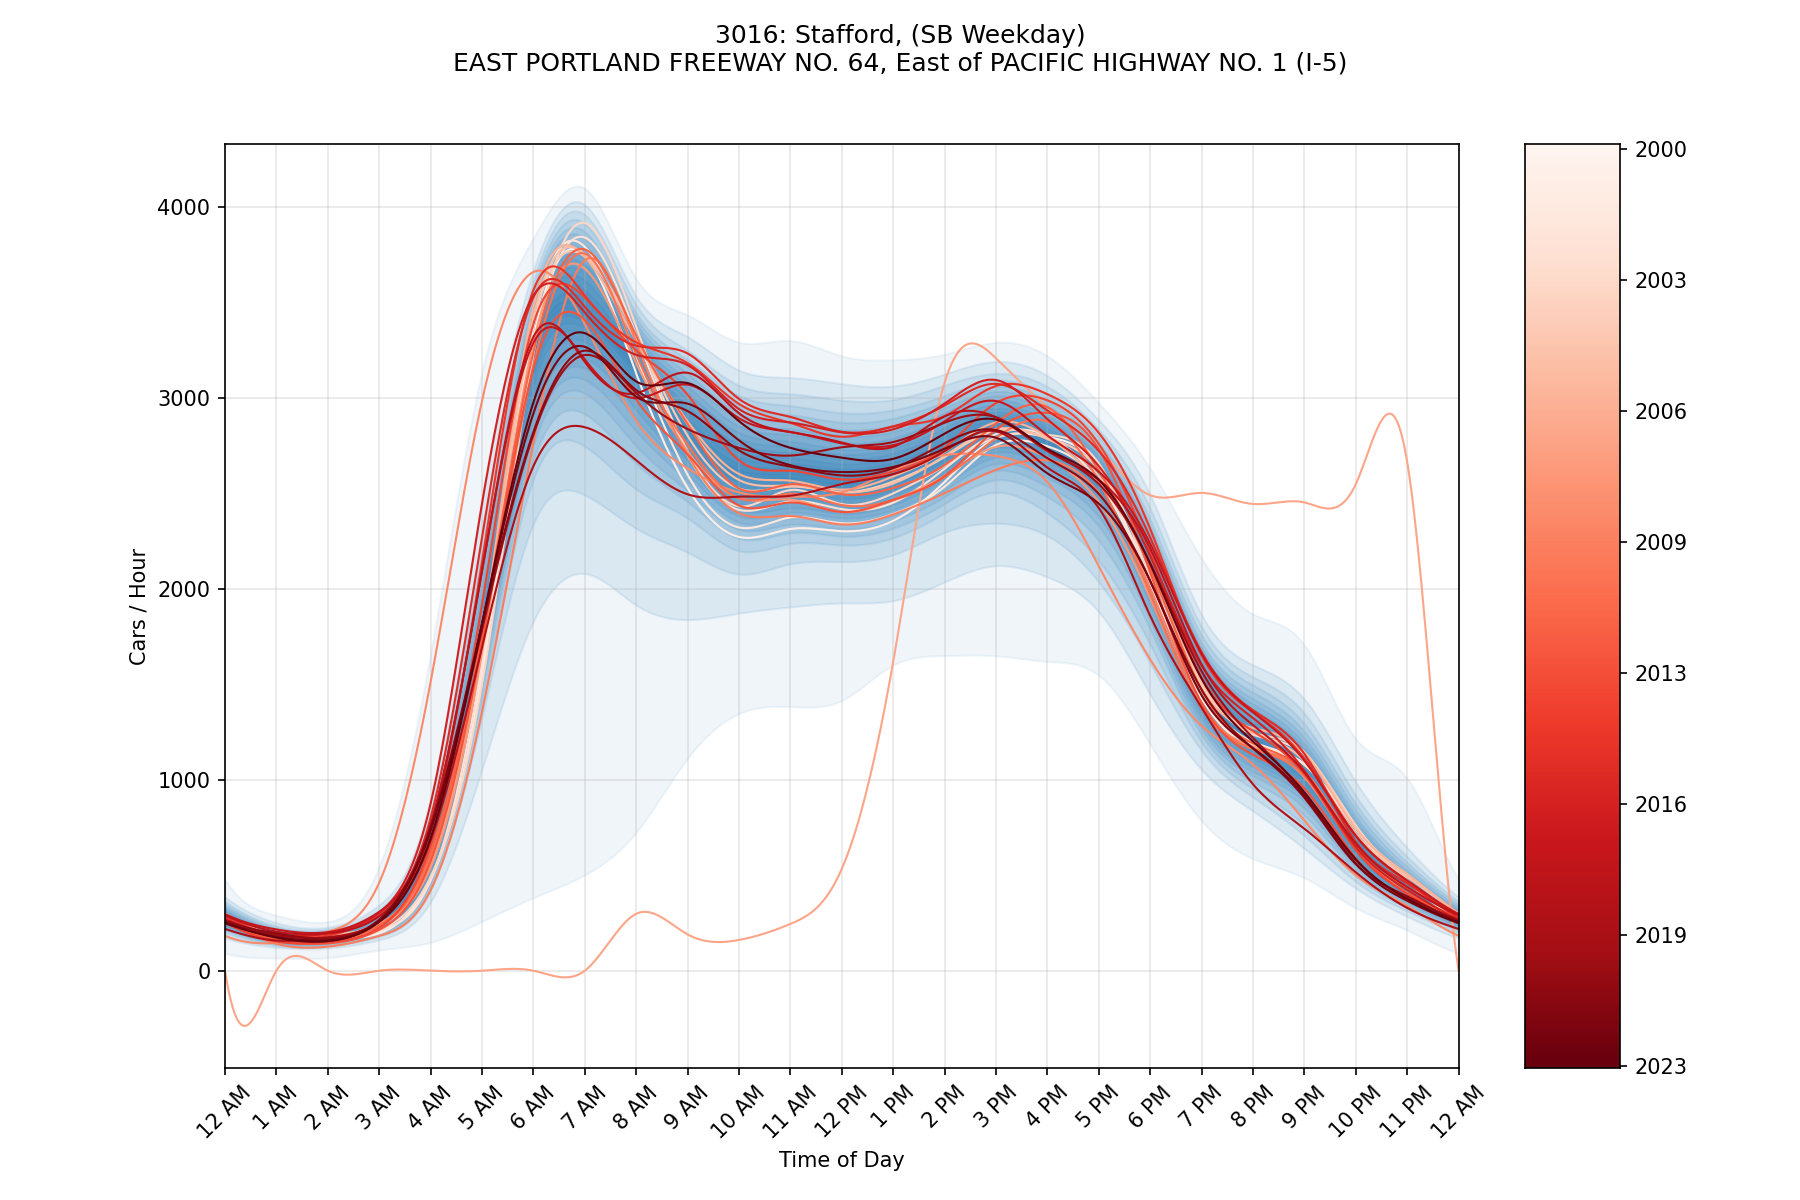
\includegraphics[width=\textwidth]{3016_Stafford_SB_Weekday.png}
	\end{subfigure}
	\hfill
	\begin{subfigure}{0.45\textwidth}
		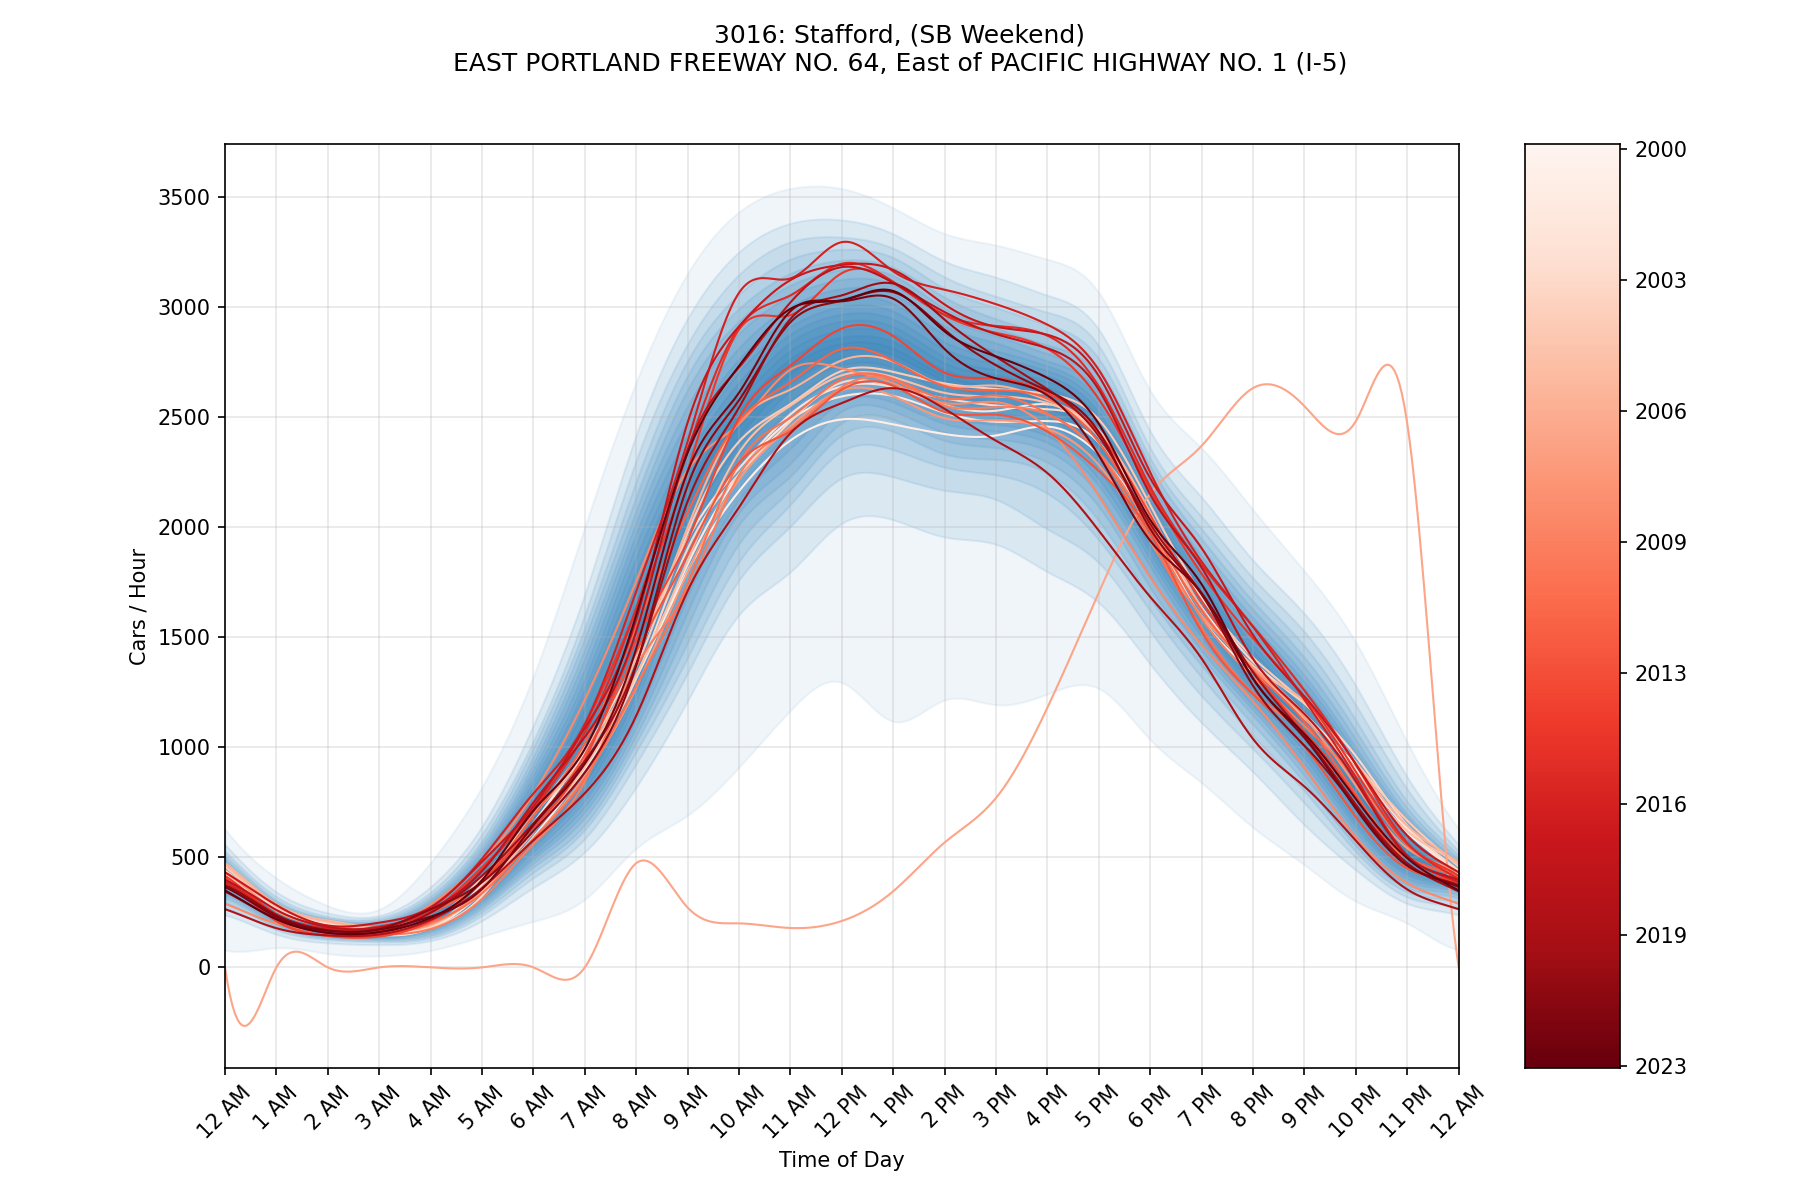
\includegraphics[width=\textwidth]{3016_Stafford_SB_Weekend.png}
	\end{subfigure}
\end{figure}

\begin{figure}[htbp]
	\centering
	\begin{subfigure}{0.45\textwidth}
		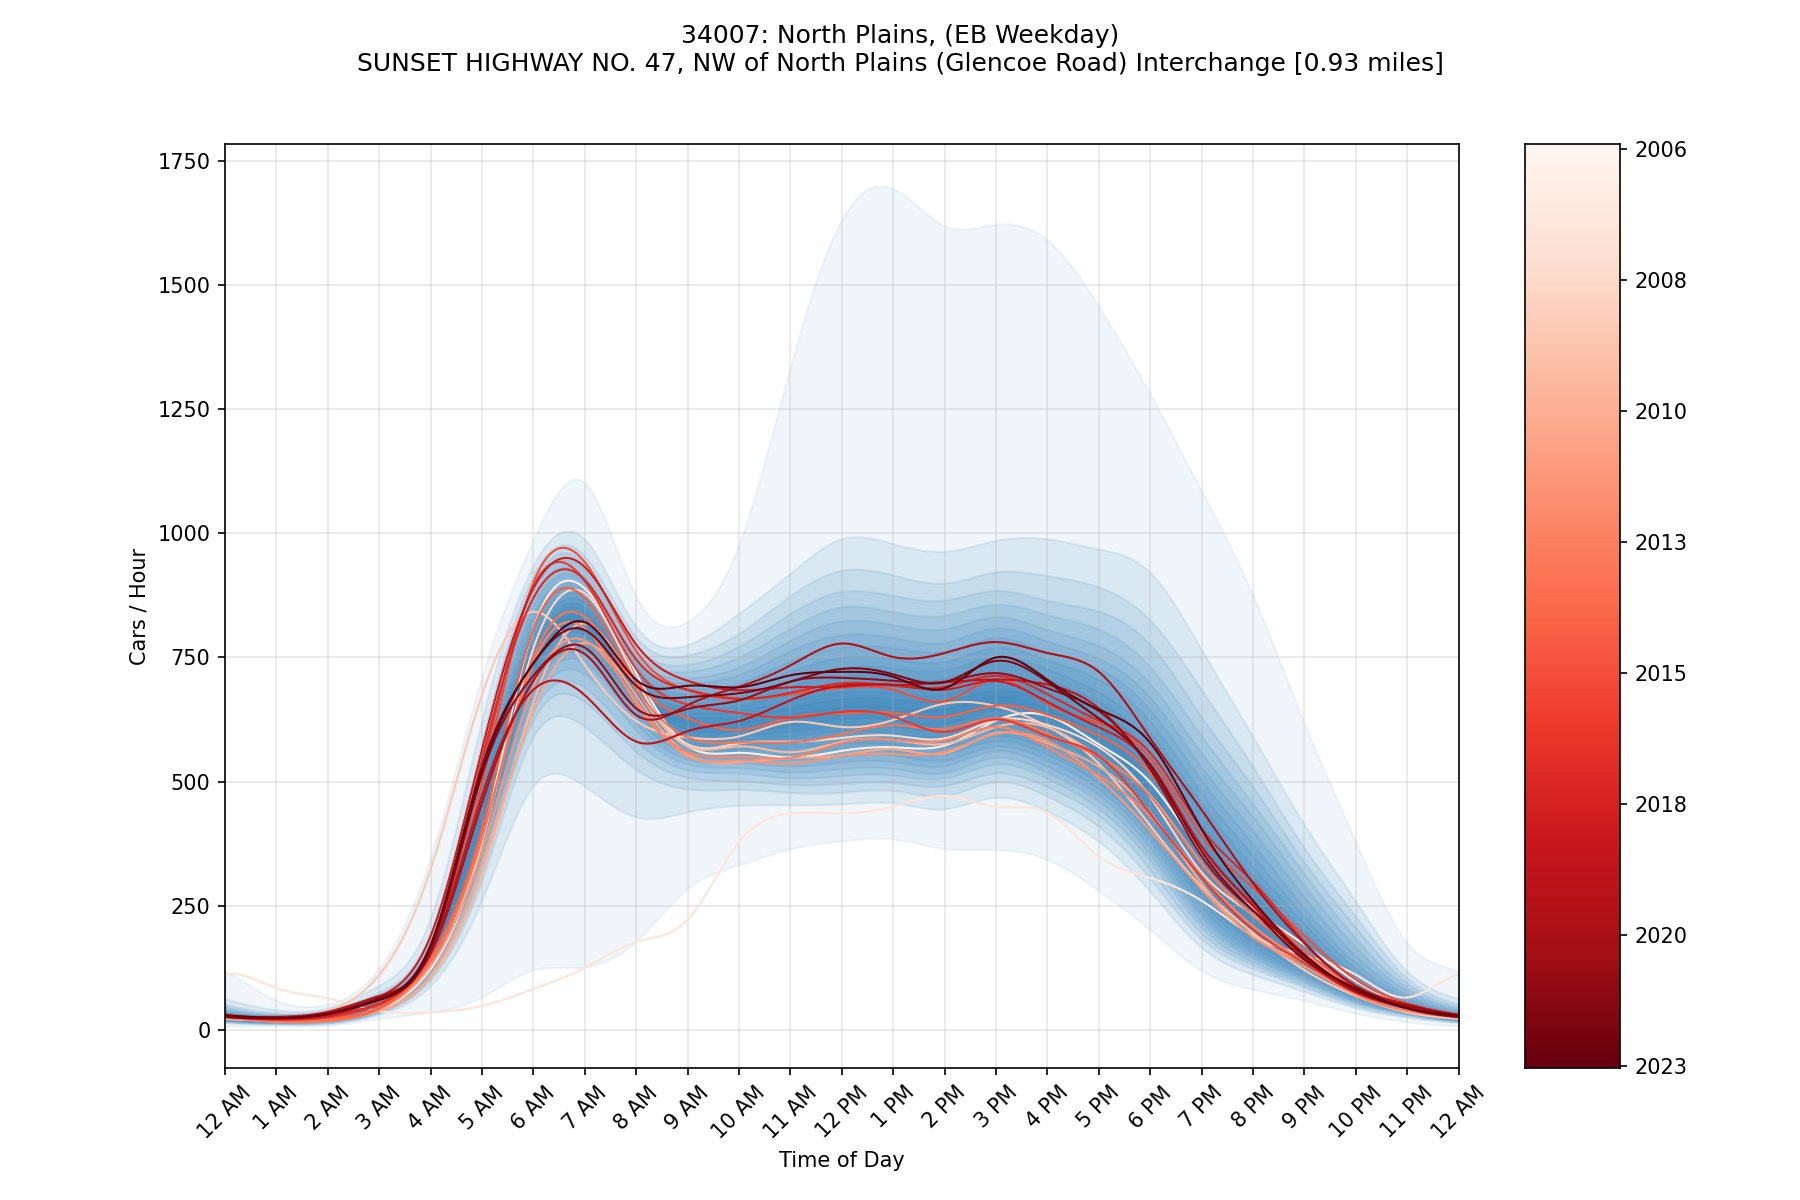
\includegraphics[width=\textwidth]{34007_North-Plains_EB_Weekday.png}
	\end{subfigure}
	\hfill
	\begin{subfigure}{0.45\textwidth}
		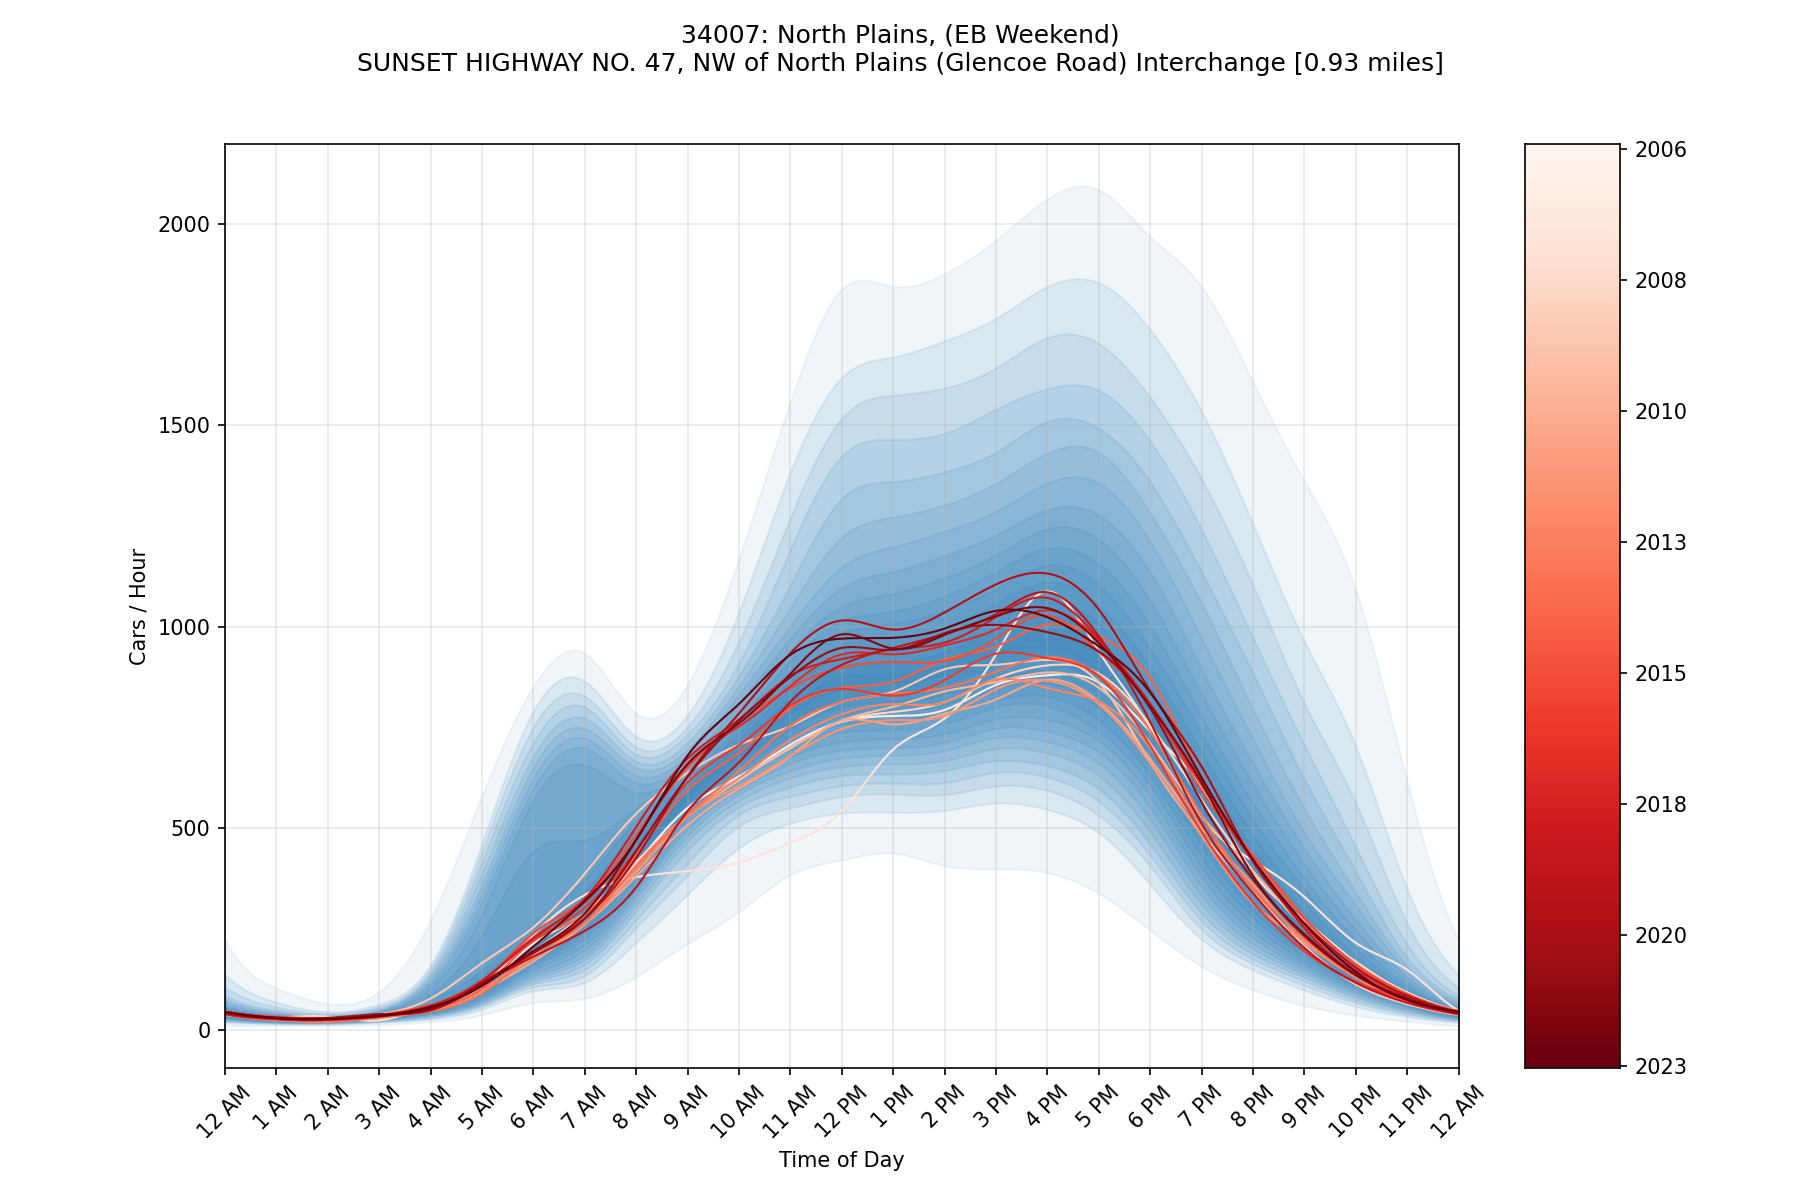
\includegraphics[width=\textwidth]{34007_North-Plains_EB_Weekend.png}
	\end{subfigure}

	\begin{subfigure}{0.45\textwidth}
		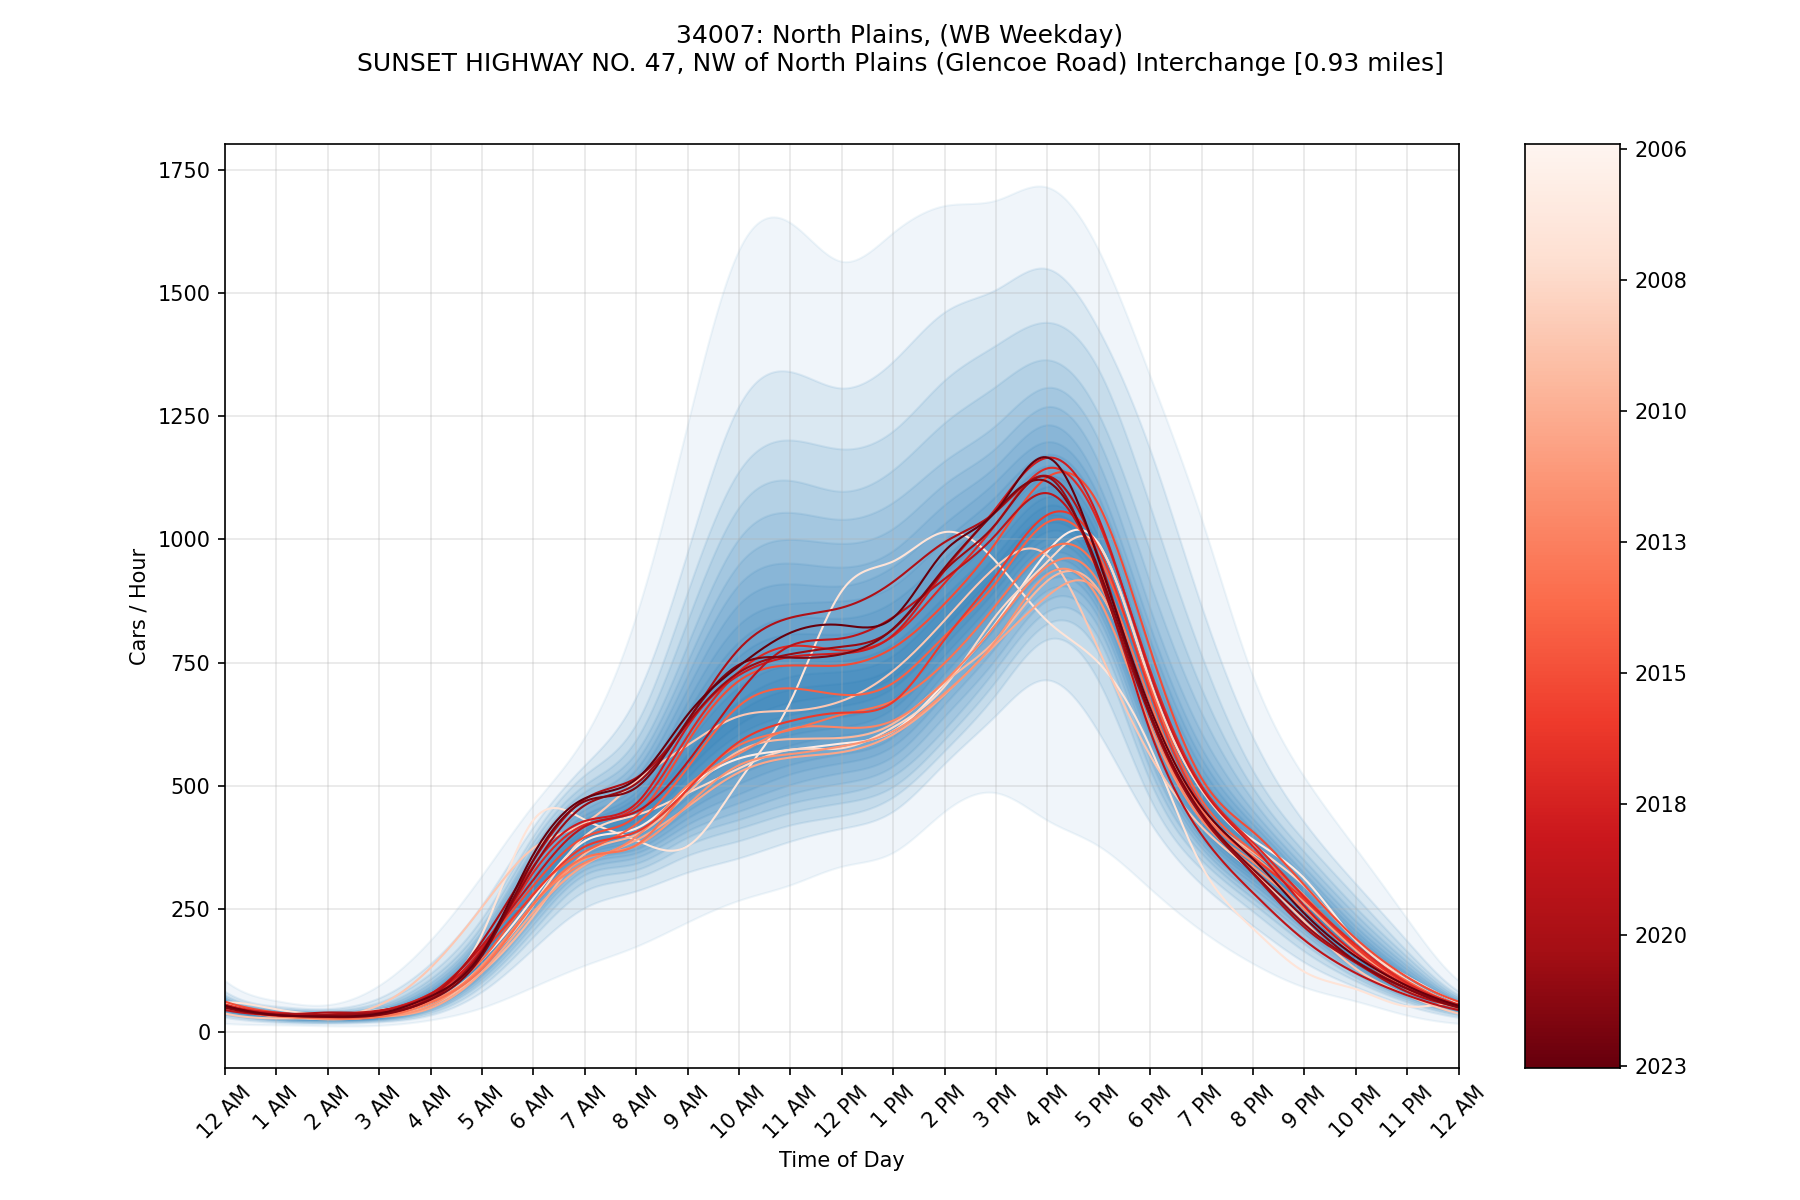
\includegraphics[width=\textwidth]{34007_North-Plains_WB_Weekday.png}
	\end{subfigure}
	\hfill
	\begin{subfigure}{0.45\textwidth}
		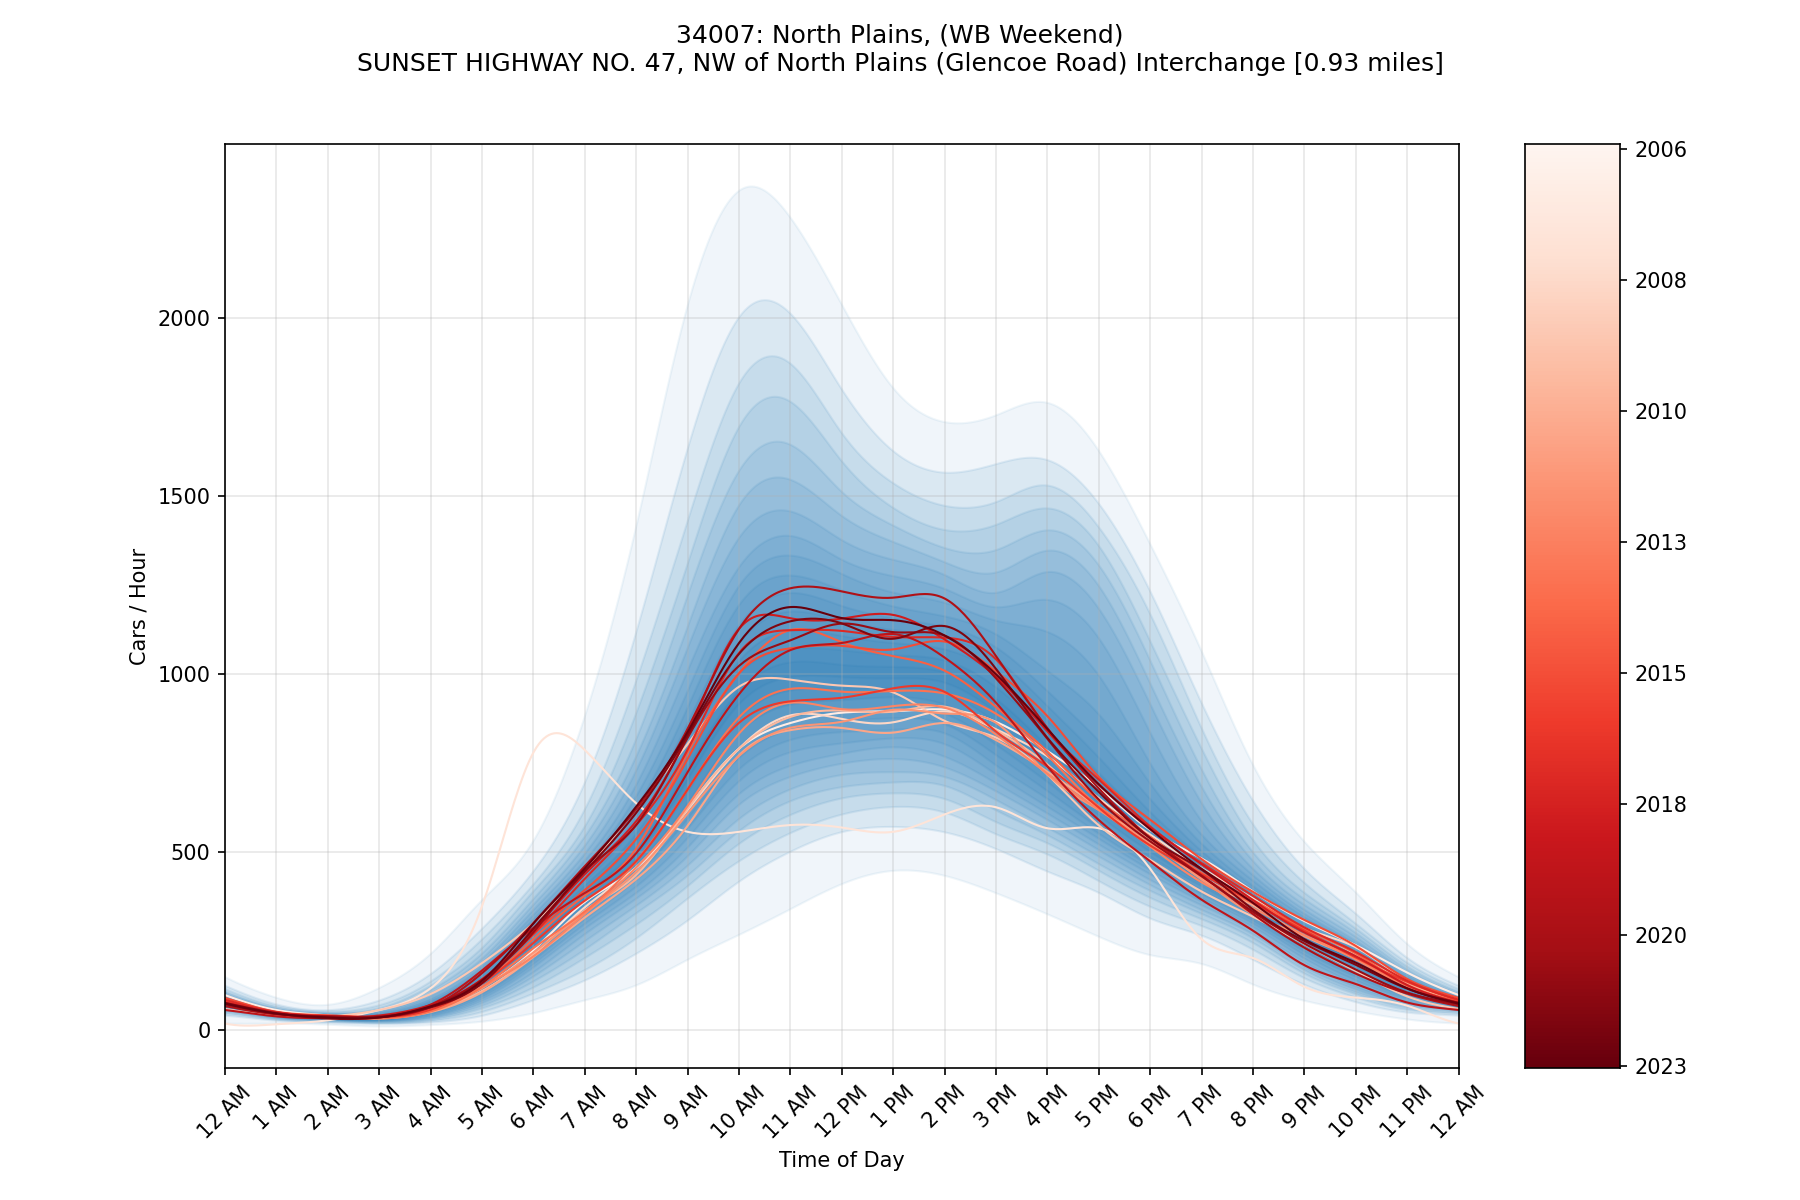
\includegraphics[width=\textwidth]{34007_North-Plains_WB_Weekend.png}
	\end{subfigure}
\end{figure}

\begin{figure}[htbp]
	\centering
	\begin{subfigure}{0.45\textwidth}
		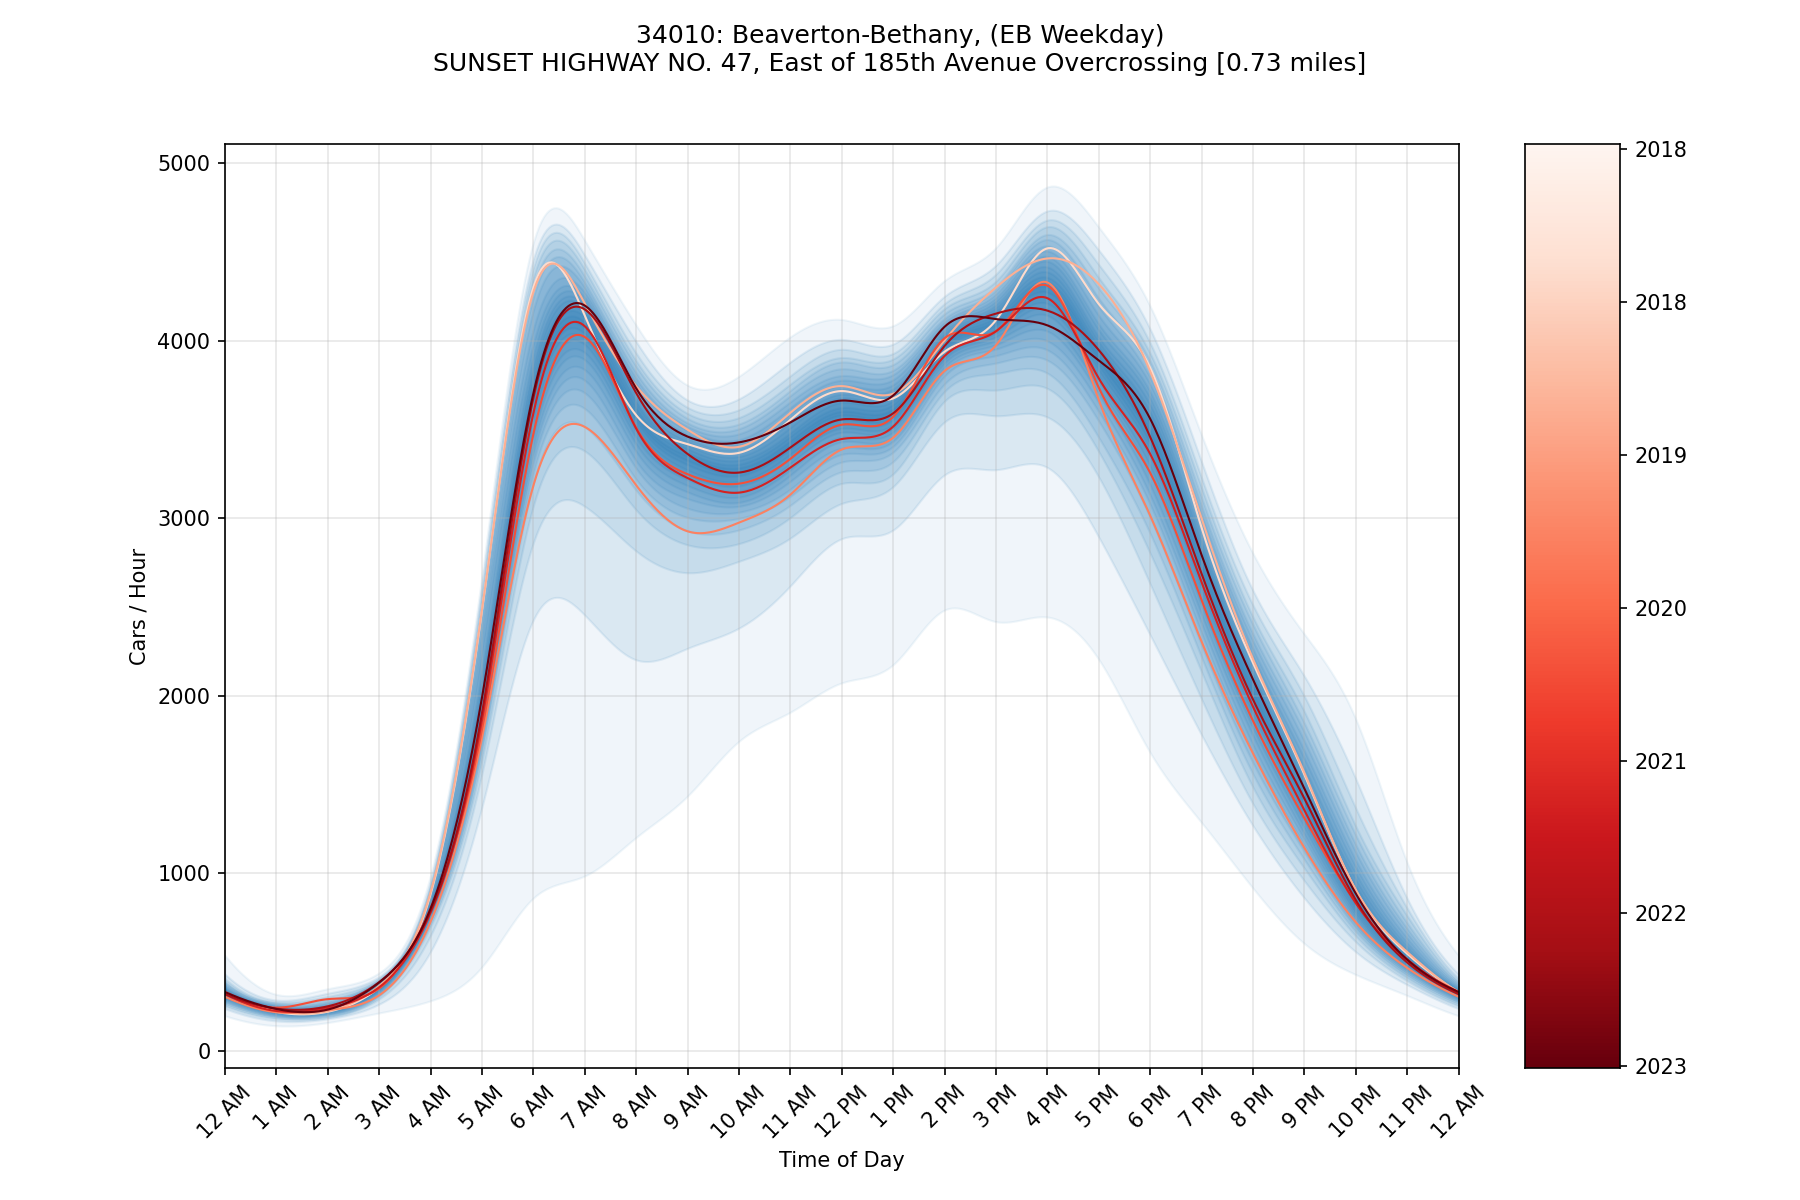
\includegraphics[width=\textwidth]{34010_Beaverton-Bethany_EB_Weekday.png}
	\end{subfigure}
	\hfill
	\begin{subfigure}{0.45\textwidth}
		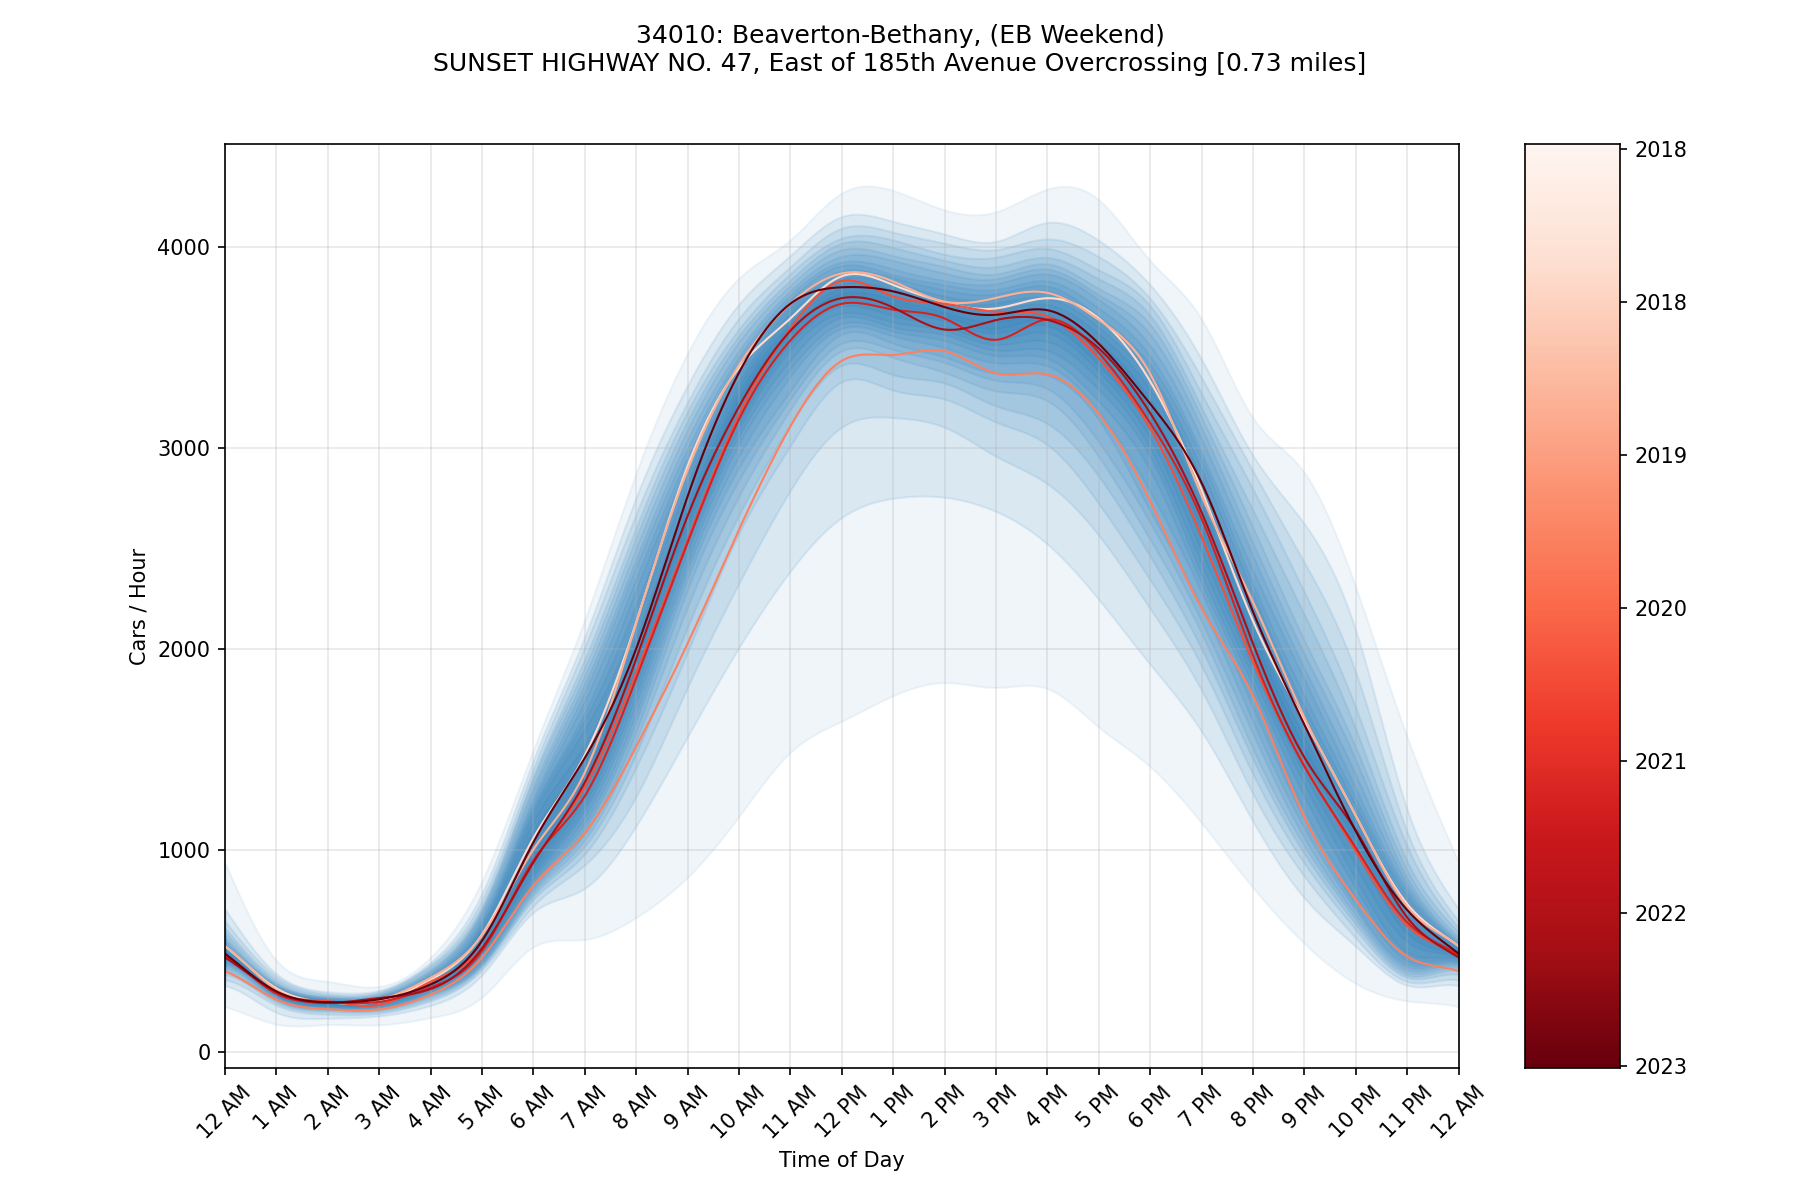
\includegraphics[width=\textwidth]{34010_Beaverton-Bethany_EB_Weekend.png}
	\end{subfigure}

	\begin{subfigure}{0.45\textwidth}
		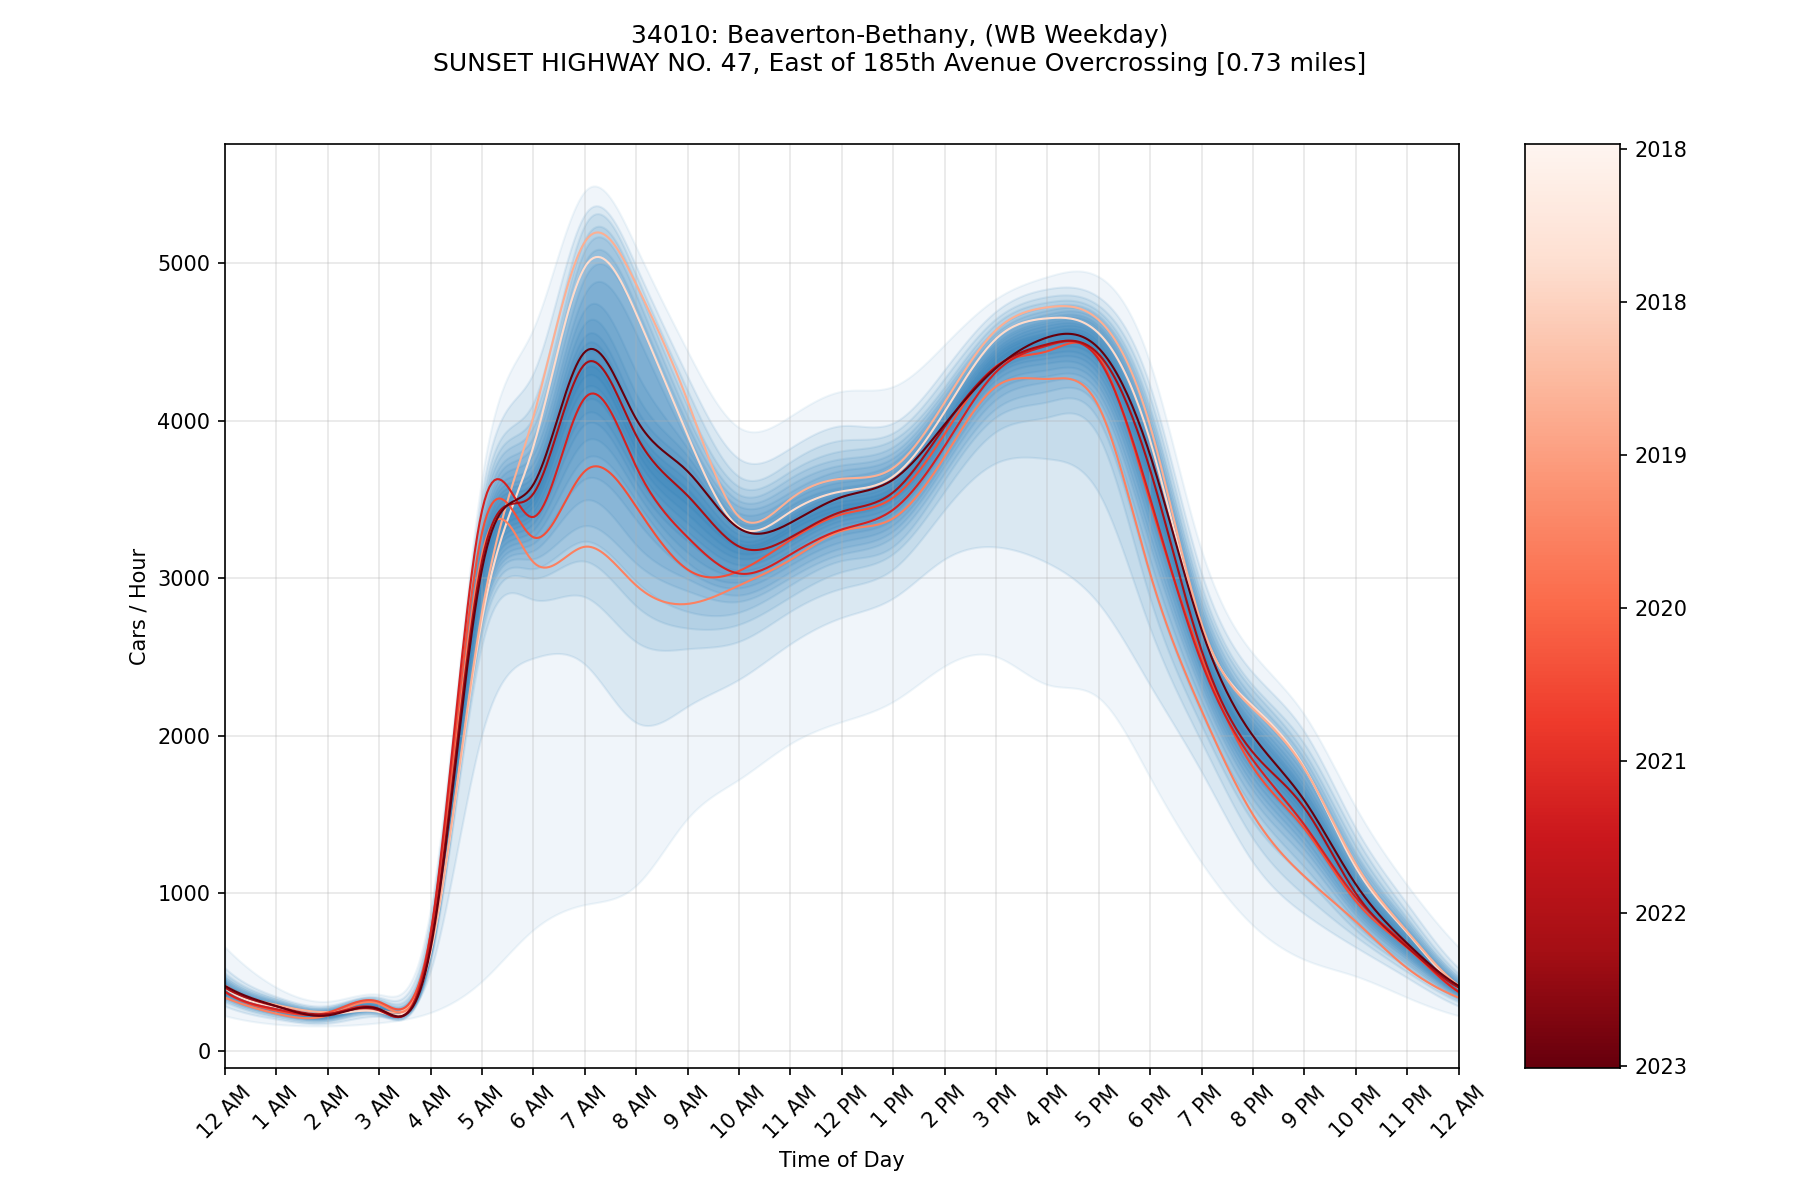
\includegraphics[width=\textwidth]{34010_Beaverton-Bethany_WB_Weekday.png}
	\end{subfigure}
	\hfill
	\begin{subfigure}{0.45\textwidth}
		\includegraphics[width=\textwidth]{34010_Beaverton-Bethany_WB_Weekend.png}
	\end{subfigure}
\end{figure}


\bibliography{references}
\end{document}

